\documentclass[eng]{kjas3}
\usepackage{amsmath, natbib}
\usepackage{graphics, graphicx, multirow, subfigure, enumerate}
\usepackage{amssymb}     % \mathbb 등
\usepackage{booktabs}    % toprule/midrule/bottomrule
\usepackage[table]{xcolor}  % 표 셀 색상
\definecolor{posgreen}{HTML}{D5E8D4}
\definecolor{negred}{HTML}{F8CECC}

% kjas3.cls does not define \paragraph; provide a minimal run-in heading.
\makeatletter
\newcommand\paragraph{\@startsection{paragraph}{4}{\z@}%
    {1.5ex \@plus1ex \@minus.2ex}%
    {-1em}%
    {\normalfont\normalsize\bfseries}}
% Suppress numeric labels for \bibitem inside the KJAS \reference list,
% so entries render like the existing \item[] style while natbib can still
% bind cite keys for \citet / \citep.
\renewcommand\@biblabel[1]{}
\makeatother

% ==================== Do not Modify here ============================
\submit{final}
\volumn{00}{0}{0000}
\receive{0000}{0}{0} \revise{0000}{0}{0}  \accept{0000}{0}{0}
\setpagenum{1}
% ====================================================================

\heading{변동성 예측을 결합한 블랙-리터만 저변동성 포트폴리오 전략}{Yoonbeom Seo, Hayeon Kim, Jaecheon Kim, Yoonseo Kim, and Jeongwook Seo}

\begin{document}

\title{Low-Volatility Black--Litterman Portfolio Strategy with Volatility Forecasts}

\author{
Yoonbeom Seo\address[a]{Team Sparta;},
Hayeon Kim\same[a],
Jaecheon Kim\same[a],
Yoonseo Kim\same[a],
Jeongwook Seo\footnote{Corresponding author:
Department of Applied Artificial Intelligence, Hanyang University,
55, Hanyangdaehak-ro, Ansan-si, 15588, Republic of Korea.
E-mail: sju02051@hanyang.ac.kr}\address[b]{Department of Applied Artificial Intelligence, Hanyang University}
}

\begin{abstract}
The Black--Litterman (BL) model mitigates estimation-error sensitivity in mean--variance optimization by combining market equilibrium with investor views, yet relies on subjective expert judgment. While machine learning--based BL applications have grown, most focus on return forecasting, leaving volatility-based views underexplored. This study extends \citet{pyo2018}'s ANN-based framework along two axes: (1) replacing ANN with an LSTM--HAR ensemble reflecting sequential dependence, and (2) systematically exploring 90 slot combinations defined by the Cartesian product of candidates for each BL input ($\mathbf{p}, q, \omega, \mathbf{w}_{mkt}$). Empirical analysis on 617 S\&P 500 constituents over 192 months (2010--2025) shows that the LSTM--HAR ensemble consistently outperforms ANN in volatility forecasting, with the largest margin during the crisis regime (R3, COVID-19 included). Translating this advantage into portfolio performance requires mitigating large-cap concentration in the view portfolio ($\mathbf{p}^{\mathrm{eq}}, \mathbf{p}^{\mathrm{rp}}$). The two proposed slot options---Ensemble-defensive (Sharpe 1.04--1.07) and Ensemble-adaptive (Sharpe 1.05--1.10)---both outperform SPY (0.93), $1/N$ (0.86), Risk Parity (0.89), and ANN-anchor (0.95) even after 20bp one-sided transaction costs.
\end{abstract}

\keywords{Black-Litterman, Volatility forecasting, LSTM, HAR, Low-volatility portfolio}

\section{서론}

마코위츠의 평균-분산 최적화(Mean-Variance Optimization, MVO, \citealp{markowitz1952}) 이래로 포트폴리오 구성 이론은 기대수익률과 위험의 절충을 다루는 방법론을 다수 발전시켜왔다. 그러나 MVO는 입력값의 추정 오차에 극도로 민감하여, 최적해가 표본 외에서 불안정하고 입력값의 작은 변화에도 극단적인 가중치를 산출한다는 한계가 지적되어 왔다. 이러한 한계에 대응하기 위해 수축(shrinkage) 추정\citep{ledoitwolf2004}, 베이지안 접근 등 다양한 후속 연구가 제안되어 왔다. 그 중 \citet{black1992}이 제안한 블랙-리터만 모형(Black-Litterman, BL) 은 시장 균형 수익률을 사전 분포로 두고 투자자의 견해(뷰, view)를 결합해 사후 기대수익률을 도출하는 베이지안 방법론으로, 추정 오차를 완화하면서도 투자 전문가의 견해를 반영하여 포트폴리오 가중치를 설정할 수 있어 폭넓게 연구되어왔다. 그러나 이 견해가 전문가의 주관적 판단에 의존한다는 한계가 존재한다.

앞선 한계를 해결하기 위해, 투자자의 뷰를 머신러닝 기반으로 예측하는 다수의 연구가 진행되어 왔다. BL 프레임워크의 핵심은 포트폴리오 뷰 $\mathbf{p}$와 기대수익률 뷰 $q$의 설정에 있으며, 머신러닝 기반 BL 응용 연구는 주로 $q$를 트리 기반, 신경망, LLM 등의 모형으로 예측하여 뷰로 주입하는 방식을 취해왔다\citep{barua2023using, su2026objective, lee2025llm}. 이들은 머신러닝 기반 수익률 예측이 BL 프레임워크의 뷰 정량화에 효과적으로 활용될 수 있음을 보였다.

한편 BL의 뷰는 반드시 기대수익률에 국한될 필요는 없다. 자산의 변동성 또한 포트폴리오 구성에서 중요한 요소이며, \citet{baker2011}, \citet{frazzini2014}, \citet{blitz2007} 등이 보고한 저위험 이상현상(저베타, 저변동 종목이 위험 대비 우수한 수익을 보이는 현상)은 변동성을 직접 뷰로 활용할 수 있는 근거를 제공한다. 다만, 본 연구는 이상현상 자체의 검증이 아닌, 현상의 존재를 출발점으로 BL 프레임워크 내에서 변동성을 신호로서 효과적으로 활용하는 방법에 초점을 둔다.

변동성 기반의 머신러닝 접근은 수익률 기반 응용 연구 대비 비교적 부족한 영역으로 남아있으며, 이 관점에서 \citet{pyo2018}는 인공신경망(Artificial Neural Network, ANN) 기반 변동성 예측을 활용해 종목을 저위험·고위험으로 분류하고, BL 뷰로 결합하는 방법을 KOSPI 200에 적용하여 BL 기반 포트폴리오가 샤프 비율(Sharpe ratio) 0.70을 달성하여 시가총액 비중(0.36) 및 시장 지수(0.59) 대비 우위를 보였다.

그러나 이 방식에는 두 가지 측면에서 추가 검토의 여지를 남긴다. 첫째, ANN 기반의 단순한 변동성 예측은 시계열 구조에 특화된 모형 구조가 아니며, 변동성의 다중 시간 척도\citep{corsi2009}와 순차적 의존성을 모형 차원에서 직접 반영하지 못해 예측 정확도에 한계가 있다. 둘째, BL 프레임워크의 운영 핵심인 포트폴리오 뷰 $\mathbf{p}$와 기대수익률 뷰 $q$의 구성이 저변동성(Low-Volatility) 포트폴리오 성과에 미치는 영향이 체계적으로 검토되지 않았다. 일반적 포트폴리오 구성 연구에서 \citet{demiguel2009optimal}, \citet{maillard2010} 등은 시가총액 대비 동일 가중(equal-weighted, eq)·리스크 패리티(risk parity, rp)가 포트폴리오 효율성 측면에서 우위를 보일 수 있음을 보고하였다. 또한, 기대수익률 뷰 $q$를 Fama-French 회귀 기반 예측값으로 산출하였으나, 해당 예측값의 부호와 크기가 저변동 포트폴리오의 성과에 미치는 영향에 대해서는 체계적인 비교·분석이 미비한 실정이다. 

본 연구는 위 두 영역에 대해 다음과 같이 기여한다. 먼저, LSTM(Long Short-Term Memory)과 HAR(Heterogeneous Autoregressive) 앙상블 모형을 적용하여 변동성의 다중 시간 척도와 순차적 의존성을 동시에 반영하는 예측 구조를 제안한다. 다음으로, BL 프레임워크의 네 가지 핵심 슬롯($\mathbf{p}, q, \omega$, $\mathbf{w}_{mkt}$)에 걸쳐 90개 조합을 체계적으로 탐색함으로써, 저변동 전략의 효과를 극대화할 수 있는 최적의 포트폴리오 슬롯 설정을 제시한다. 이는 비시계열 모형과 고정된 슬롯 구성에 의존했던 선행 연구\citep{pyo2018}를 예측 모형과 포트폴리오 구조 설계라는 두 가지 축 모두에서 유의미하게 확장하였다는 점에서 차별성을 갖는다.

본 연구는 다음과 같은 순서로 구성된다. \ref{sec:related_work}절에서는 변동성 예측 및 BL 응용에 관한 선행 연구를 검토하고, \ref{sec:method}절에서는 본 연구의 변동성 예측 모형과 BL 프레임워크의 구조 및 슬롯 구성을 기술한다. \ref{sec:result}절에서는 실증 분석 결과를 제시하고, 마지막 \ref{sec:conclusion}절에서는 연구 결론과 한계점을 논의한다.

\section{선행 연구}\label{sec:related_work}

\subsection{블랙-리터만}
\label{subsec:bl_review}

블랙-리터만 모형(Black–Litterman, BL, \citealp{black1992}) 은 시장 균형 수익률과 투자자의 뷰를 베이지안 방식으로 결합하는 포트폴리오 최적화 프레임워크로, MVO가 갖는 추정 오차 민감성을 완화하는 데 효과적이다. 모형은 이차 효용 최대화 문제의 역산으로 도출되는 시장 균형 초과수익률 벡터 $\boldsymbol{\pi}$에서 출발한다.

\begin{align}\label{eq:bl_pi}
    & \boldsymbol{\pi} = \lambda\boldsymbol{\Sigma}\mathbf{w}_{mkt}
\end{align}

여기서 $\boldsymbol{\pi} \in \mathbb{R}^{n \times 1}$은 균형 초과수익률 벡터, $\boldsymbol{\Sigma}\in \mathbb{R}^{n \times n}$은 초과수익률 공분산 행렬, $\mathbf{w}_{mkt} \in \mathbb{R}^{n \times 1}$은 시장 비중 벡터, $\lambda$는 시장 위험회피계수이다. $\lambda$는 모형 외부에서 주어지는 하이퍼파라미터로, \citet{helitterman1999}은 미국 주식시장의 역사적 위험-수익 관계로부터 $\lambda \approx 2.5$를 제안하였으며, 이후 BL 응용 문헌의 표준값으로 널리 채택되었다. 공분산 행렬 $\boldsymbol{\Sigma}$의 추정은 자산 수 $n$이 표본 길이 $T$ 에 비해 클 때 표본 공분산이 큰 추정 오차를 갖는다는 문제가 알려져 있다. \citet{ledoitwolf2004}는 표본 공분산을 구조화된 타깃과 선형 결합하는 수축(shrinkage) 추정량을 제안하여 이 문제를 완화하였으며, 이후 고차원 포트폴리오 추정에서 폭넓게 활용되어 왔다.

사전 분포(prior)는 다음과 같이 설정된다.

\begin{align}\label{eq:bl_mu}
    \boldsymbol{\mu} \sim N(\boldsymbol{\pi}, \tau\boldsymbol{\Sigma})
\end{align}

$\tau$는 사전 분포의 불확실성을 조절하며, \citet{helitterman1999}은 사전 분포에 약한 신뢰도를 부여할 때 $\tau$를 작은 값(0.025\textendash 0.1)으로 두는 관행을 확립하였다.

투자자의 뷰는 다음과 같이 표현된다.

\begin{align}\label{eq:bl_q}
    q|\boldsymbol{\mu} \sim N(\mathbf{p}\boldsymbol{\mu}, \omega)
\end{align}

여기서 $\mathbf{p} \in R^{1 \times n}$은 뷰 포트폴리오 가중치 벡터, $q \in R$은 단일 상대 뷰의 기대수익률 스칼라, $\omega\in R$는 뷰의 불확실성을 나타내는 스칼라다. $\omega$의 구체적 형태는 BL 응용 문헌에서 다양하게 논의되었으며, \citet{helitterman1999}은 $\omega = \tau\mathbf{p}\boldsymbol{\Sigma}\mathbf{p}^\top$와 같이 사전 분포의 공분산에 비례하는 형태를 표준으로 제시하였다.

사전 분포와 뷰 우도를 결합하면 사후 기대수익률과 공분산은 다음과 같이 도출된다.

\begin{align}\label{eq:bl_sigma_pos}
    & \boldsymbol{\Sigma}_{BL} = [(\tau\boldsymbol{\Sigma})^{-1} + \mathbf{p}^\top\omega^{-1}\mathbf{p}]^{-1}\\
    \label{eq:bl_mu_pos}
    & \boldsymbol{\mu}_{BL} = [(\tau\boldsymbol{\Sigma})^{-1} + \mathbf{p}^\top\omega^{-1}\mathbf{p}]^{-1}[(\tau\boldsymbol{\Sigma})^{-1}\boldsymbol{\pi}+\mathbf{p}^\top\omega^{-1}q]
\end{align}

최적 포트폴리오 비중은 다음을 풀어 산출한다.

\begin{align}\label{eq:bl_w}
    \min_{\mathbf{w}}\frac{1}{2}\lambda\mathbf{w}^\top\boldsymbol{\Sigma}_{BL}\mathbf{w}-\mathbf{w}^\top\boldsymbol{\mu}_{BL} \\
\text{s.t.} \quad \sum_{i=1}^{n}{w_i} = 1
\end{align}

\subsection{변동성 예측 모형}
\label{subsec:vol_pred_review}

금융 자산의 변동성은 시계열적으로 특정 구조가 지속되는 '변동성 군집성(volatility clustering)'과 시차가 길어져도 자기상관이 천천히 감소하는 '장기 의존성(long-memory)'을 보인다\citep{cont2001}. 본 절에서는 이러한 변동성 시계열 구조에 널리 활용되어 온 선형 모형인 HAR\citep{muller1997}과 비선형 시퀀스 학습에 특화된 딥러닝 모형인 LSTM\citep{hochreiter1997}의 구조를 기술한다. 아울러 서로 다른 가정에 기반한 두 모형의 예측값을 결합함으로써 동적 적응성(dynamic adaptability)을 확보하는 앙상블 접근법의 이론적 배경을 정리한다.

\subsubsection{HAR}
\label{subsubsec:har_review}

\citet{muller1997}은 시장 참여자의 의사결정 시간 지평(time horizon)이 단기·중기·장기로 이질적이라는 '이질적 시장 가정(Heterogeneous Market Hypothesis)'을 제안하였다. 이 가정에 따르면, 변동성의 장기 의존 구조는 서로 다른 시간 척도를 가진 거래 행동이 중첩된 결과로 해석된다. 
\citet{corsi2009}은 이를 단순 선형 회귀 형태로 구현한 HAR 모형을 개발하였다. HAR 모형은 시차(lag)를 개별적으로 나열하는 대신, 단기(1일), 중기(5일), 장기(22일) 누적 평균 실현분산(Realized Volatility, RV)을 입력 변수로 사용한다. 이를 통해 단 네 개의 모수(parameter)만으로도 복잡한 자기상관 구조를 효과적으로 근사한다는 장점이 있다.

\begin{equation}
\log RV_{h,t+h} = \beta_0 + \beta_d \log RV_{d,t} + \beta_w \log RV_{w,t} + \beta_m \log RV_{m,t} \label{eq:har_full}
\end{equation}

여기에서 $(RV_d, RV_w, RV_m)$는 1일, 5일, 22일에 걸친 변동성 대리변수이다. HAR 모형은 구조적 단순성에도 불구하고 변동성의 장기 의존 구조를 효과적으로 포착하여 변동성 연구의 대표적인 벤치마크로 자리 잡았다.

\subsubsection{LSTM}
\label{subsubsec:lstm_review}

순환신경망(Recurrent Neural Network, RNN, \citealp{rumelhart1986learning})은 시퀀스 데이터의 시간적 의존성을 학습하기 위해 은닉 상태(hidden state) $h_t$를 시점 간 재귀적으로 전파하는 구조를 갖는다. 그러나 RNN은 역전파 과정에서 기울기가 시간 축을 따라 지수적으로 감소하거나(기울기 소실, vanishing gradient) 지수적으로 증가하는(기울기 폭주, exploding gradient) 문제로 인해, 긴 시퀀스 학습이 실질적으로 어렵다는 한계가 지적되어 왔다.

LSTM\citep{hochreiter1997}은 이러한 한계를 해결하기 위해 설계된 구조이다. LSTM의 핵심 아이디어는 은닉 상태와 별도로 셀 상태(cell state) $c_t$를 두고, [0, 1] 구간의 출력값을 갖는 시그모이드 활성화 함수를 통해 셀 상태의 정보를 선택적으로 보존·삭제·갱신하는 것이다. \citet{gers2000}이 망각 게이트(forget gate)를 도입한 이후, LSTM은 망각·입력·출력 게이트 및 후보 기억 상태(candidate cell state)로 구성된 표준 구조로 정착하였다.

\begin{figure}[t]
\centering
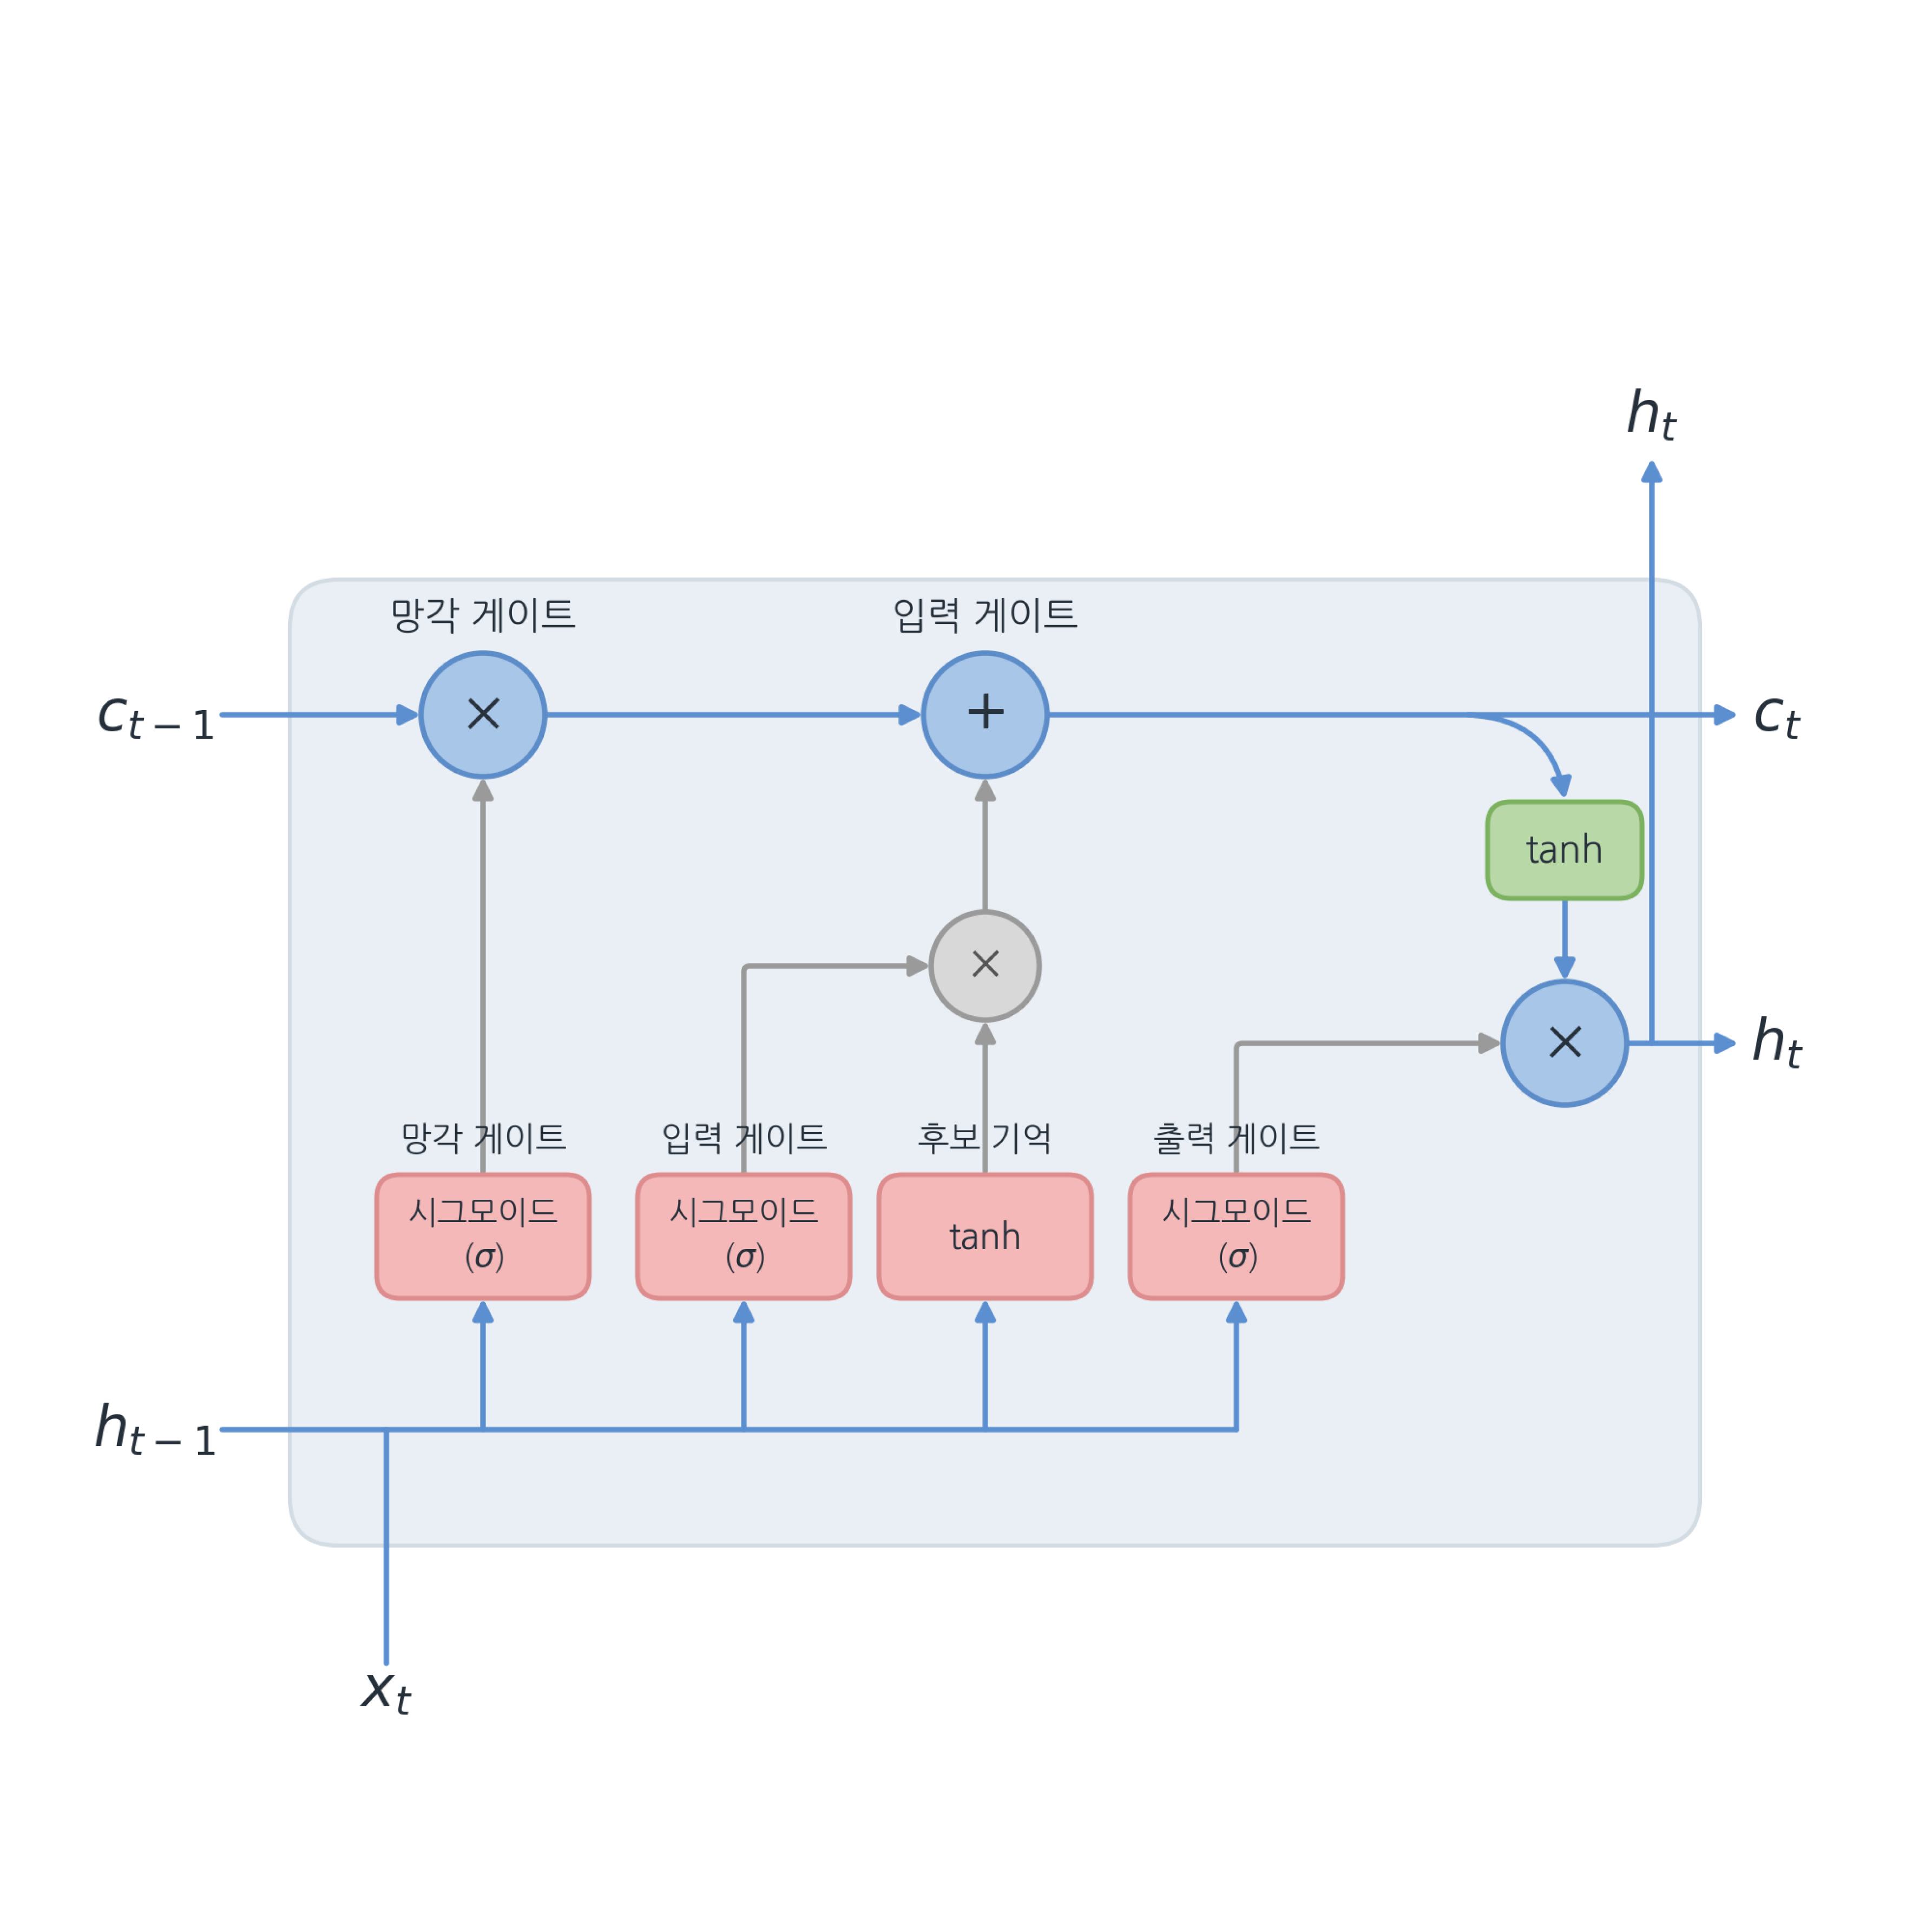
\includegraphics[width=0.75\textwidth]{Figure/lstm_cell.png}
\caption{LSTM 셀의 내부 구조.}
\label{fig:lstm_cell}
\end{figure}

그림~\ref{fig:lstm_cell}의 LSTM 셀은 시점 $t$에서 다음과 같이 계산된다.
\begin{align}
f_t &= \sigma(W_f [h_{t-1}, x_t] + b_f) \label{eq:lstm_f}\\
i_t &= \sigma(W_i [h_{t-1}, x_t] + b_i) \label{eq:lstm_i}\\
\tilde{c}_t &= \tanh(W_c [h_{t-1}, x_t] + b_c) \label{eq:lstm_ctilde}\\
c_t &= f_t \odot c_{t-1} + i_t \odot \tilde{c}_t \label{eq:lstm_c}\\
o_t &= \sigma(W_o [h_{t-1}, x_t] + b_o) \label{eq:lstm_o}\\
h_t &= o_t \odot \tanh(c_t) \label{eq:lstm_h}
\end{align}
여기서 $f_t$, $i_t$, $o_t$는 각각 망각·입력·출력 게이트, $\tilde{c}_t$는 후보 기억 상태를 나타낸다. $\sigma(\cdot)$은 시그모이드 활성화 함수, $\tanh(\cdot)$는 하이퍼볼릭 탄젠트 활성화 함수, $\odot$ 은 원소별 곱(Hadamard product)이다. 또한 \(W\)와 \(b\)는 각 구성 요소의 가중치 행렬과 편향 벡터를 나타내며, \([h_{t-1}, x_t]\)는 은닉 상태와 입력 벡터의 결합(concatenation)을 의미한다. 식~(\ref{eq:lstm_c})의 망각 게이트 $f_t$가 1에 가까울 때 과거 셀 상태가 보존되고 0에 가까울 때 폐기되어, 시계열 장기 의존 구조를 선택적으로 보존하거나 제거할 수 있다.

LSTM은 자연어 처리, 음성 인식 등 시퀀스 학습 문제에서 폭넓게 활용되어 왔으며, 금융 변동성 예측에 적용한 연구들도 다수 보고되었다\citep{bucci2020realized, kim2018forecasting}. 해당 연구들은 LSTM이 변동성 시계열의 비선형 구조를 학습하여 예측에 유의미하게 활용될 수 있음을 보였다.

\subsubsection{예측 앙상블}
\label{subsubsec:ens_review}

각 모형의 예측 결과를 결합하여 단일 모형 대비 오차를 줄이고자 하는 예측 결합(forecast combination, 이하 앙상블)은 \citet{bates1969combination} 이래로 활발히 연구되어 왔다. 두 예측의 가중 평균이 개별 예측보다 작은 평균제곱오차(Mean Squared Error, MSE)를 갖기 위한 이론적 조건을 분석한 이 연구는, 두 예측 오차 간의 상관관계가 낮을수록 결합을 통한 분산 감소 효과가 커진다는 점을 확인하였다.

이후의 연구는 \citet{bates1969combination}이 제안한 역분산 가중을 다양한 오차 척도로 확장한 변형들을 발전시켜 왔으며\citep{timmermann2006forecast}, 본 연구에서 채택하는 성과 가중(performance-weighted) 결합 방식 역시 이러한 발전 형태 중 하나이다. 구체적으로 각 모형의 과거 예측 오차에 반비례하도록 가중치를 부여하는 적응적 특성을 지닌다.

\begin{equation}
w_i = \frac{1/e_i}{\sum_{j=1}^{M} 1/e_j}
\label{eq:perf_weight_general}
\end{equation}

여기서 $e_i$는 모형 $i$의 과거 예측 오차(MSE 등)이며, $M$은 결합 대상이 되는 총 모형의 개수이다. 이러한 가중치 구조는 시장 국면 변화에 따라 상대적으로 우수한 성능을 보인 모형의 비중이 자동으로 조정되는 적응적 특성을 가진다.

본 연구에서 결합하는 HAR 모형과 LSTM 모형은 서로 다른 이론적 가정에 기반하고 있다. HAR 모형은 변동성을 단·중·장기 변동성 대리변수의 선형 회귀로 모형화하는 반면, LSTM은 선형성 가정 없이 데이터로부터 비선형 의존 구조를 직접 학습한다. 이처럼 매커니즘이 다른 두 모형은 서로 다른 시장 국면에서 오차를 발생시킬 가능성이 크며, 따라서 두 모형의 앙상블을 통해 단일 모형 대비 더욱 안정적이고 강건한(robust) 예측 성능을 기대할 수 있다.

\subsubsection{Walk-Forward 교차 검증}
\label{subsubsec:walk_forward_review}

머신러닝 모형의 성능 평가에서 일반적으로 사용되는 무작위 $k$-fold 교차검증은 시계열 데이터에 적용할 경우 미래 정보가 학습 구간에 노출되는 미래 참조 편향(look-ahead bias) 문제를 발생시킨다. 이는 모형이 실제 운영 환경에서는 알 수 없는 정보를 학습에 반영하게 함으로써, 평가 구간(Out-of-Sample, OOS) 성능을 과대 평가하는 결과로 이어진다.

이러한 한계를 극복하기 위해 금융 시계열 예측에서는 학습 구간(In-Sample, IS)과 평가 구간(OOS)을 시간 순서대로 분리하고, 시점을 일정 간격으로 전진시키며 반복 평가하는 Walk-Forward 교차 검증 방식이 활용되어 왔다. 그러나 종속변수가 미래 구간으로 정의되는 경우(본 연구의 경우 향후 21 영업일 수익률 표준편차), IS의 마지막 시점이 포함하는 예측 타깃(forward target)이 OOS 구간의 예측 변수와 시간적으로 중첩되어 잔여 정보가 누설되는 문제(data leakage)가 발생하게 된다.

\citet{lopezdeprado2018}은 이와 같은 잔여 정보 누설을 차단하기 위해 퍼징(Purging)과 엠바고(Embargo) 절차를 결합한 확장된 Walk-Forward 구조를 제안하였다. 퍼징은 IS 종료 직후 타깃 윈도우가 OOS와 겹치는 일정 구간의 표본을 학습에서 배제함으로써 타깃의 시간적 중첩으로 인한 왜곡을 제거하고, 엠바고는 OOS 시작 지점 직전에 추가 안전구간(embargo window)을 두어 시계열 종속변수의 자기상관(autocorrelation)이 충분히 감쇠한 이후에 OOS 평가를 시작하도록 통제한다.

\subsection{블랙-리터만과 변동성 예측의 결합}
\label{subsec:bl_vol_review}

변동성 예측 결과를 BL의 뷰로 활용하는 시도는 머신러닝 기반 수익률 예측 연구에 비해 상대적으로 미진한 편이었다. \citet{pyo2018}는 변동성 예측을 BL 뷰로 직접 활용한 선행 연구이며, 본 연구의 출발점에 해당한다. 해당 선행 연구는 (i) 종목별 변동성 예측, (ii) 예측 결과를 활용한 BL 뷰로 결합, (iii) 결합된 사후 기대수익률에 기반한 포트폴리오 비중 최적화의 세 단계로 전개된다.

\citet{pyo2018}는 KOSPI 200 종목 각각에 대해 직전 10개월의 월별 변동성을 입력 변수로 활용하여 익월 변동성을 예측한다. 변동성 예측 모형으로 ANN, 가우시안 프로세스 회귀(Gaussian Process Regression, GPR), 서포트 벡터 회귀(Support Vector Regression, SVR), 그리고 GARCH 모형을 비교·평가하였으며, 예측 편차 측면에서 가장 안정적인 성능을 보인 ANN을 최종 예측 모형으로 채택하였다.

변동성 예측 결과를 기반으로 종목을 저변동(변동성 하위 30\%)·고변동(변동성 상위 30\%) 두 그룹으로 분류한 후, 투자 뷰 벡터 $\mathbf{p}$의 개별 요소  $p_i^{mcap}$은 다음과 같이 매수-매도(long-short) 형태로 구성된다.
\begin{equation}
    p_i^{mcap} = \begin{cases}
    +\dfrac{\mathrm{mcap}_i}{\sum_{j \in \mathcal{L}} \mathrm{mcap}_j},  & \text{종목 } i \in \mathcal{L} \text{ (저변동 그룹, 하위 30\%)} ,\\[8pt]
    -\dfrac{\mathrm{mcap}_i}{\sum_{j \in \mathcal{H}} \mathrm{mcap}_j}, & \text{종목 } i \in \mathcal{H} \text{ (고변동 그룹, 상위 30\%)}, \\[6pt]
    \phantom{+}0,                & \text{otherwise}.
\end{cases}
    \label{eq:pyo_p}
\end{equation}
여기서 $\mathrm{mcap}_i$는 종목 $i$의 시가총액이며, 각 그룹 내 시가총액 합계로 정규화하여 롱(Long) 측 합은 $+1$, 숏(Short) 측 합은 $-1$이 되는 자기자금조달(self-financing) 구조를 충족한다. 기대수익률 뷰 $q$는 Fama-French 3팩터 모형(FF3, \citep{fama1993common})의 회귀 추정치와 $\mathbf{p}$의 결합으로 산출된다.

\begin{align}
\hat{r}_i &= \alpha + \beta_{\text{mkt}}(r_{\text{mkt}} - r_f)
           + \beta_{\text{smb}} \cdot \text{SMB}
           + \beta_{\text{hml}} \cdot \text{HML} \label{eq:pyo_ff3}\\
q &= \mathbf{p} \hat{\mathbf{r}} \label{eq:pyo_q}
\end{align}

뷰 신뢰도 $\omega$는 직전 시점에서 뷰의 예측 수익률과 실현 수익률 차이의 분산으로 정의된다.
\begin{equation}
\omega = \mathrm{var}\bigl(\mathbf{p}_{t-1} \hat{\boldsymbol{\mu}}_{t-1}
       - \mathbf{p}_{t-1} \boldsymbol{\mu}_{t-1}\bigr)
\label{eq:pyo_omega}
\end{equation}
이는 뷰의 신뢰도를 직전 시점의 데이터로부터 경험적으로 추정하는 방식이다.

이렇게 구성된 $(\mathbf{p}, q, \omega)$를 BL의 사후 기대수익률 $\boldsymbol{\mu}_{BL}$과 공분산 $\boldsymbol{\Sigma}_{BL}$ (식~\eqref{eq:bl_sigma_pos}, \eqref{eq:bl_mu_pos})에 대입하여 식~\eqref{eq:bl_w}로부터 최종 포트폴리오 자산 배분 비중을 산출한다.

KOSPI 200 종목을 대상으로 한 실증 분석에서 BL 기반 포트폴리오는 샤프 비율 0.70을 달성하여 시가총액 가중 포트폴리오 (0.36) 및 KOSPI 200 지수 (0.59) 대비 우위를 보였다. 이는 변동성 예측을 BL 뷰로 활용하는 접근의 실증적 근거를 제시하였다.

\section{방법론}\label{sec:method}

\subsection{전체 파이프라인}\label{subsec:pipeline}

본 연구는 앞서 \ref{subsec:bl_vol_review}절에서 서술한 \citet{pyo2018}의 분석 프레임워크를 기반으로 하되, 다음 두 가지 핵심적인 측면에서 본 연구의 차별성을 확보한다.

첫째, 금융 시계열의 특성을 반영할 수 있는 예측 모형의 고도화이다. \citet{pyo2018}에서 활용된 ANN은 시계열 구조에 특화되지 않은 단순 전방향(Feed-forward) 신경망 구조라는 한계가 있으므로, 본 연구는 이를 \ref{subsec:vol_pred_review}절에서 언급한 LSTM과 HAR 모형의 앙상블 구조로 대체한다. 다만, 선행 연구와의 통제된 비교를 위해 ANN을 동일한 환경에서 기준 모형으로 함께 평가한다.

둘째, BL 뷰 설정 슬롯의 확장이다. \citet{pyo2018}은 포트폴리오 뷰 $\mathbf{p}$, 기대수익률 뷰 $q$, 뷰 신뢰도 $\omega$, 사전 분포 $\mathbf{w}_{mkt}$를 단일 설정으로 고정한 반면, 본 연구는 이 네 축을 각각 복수의 후보로 정의한 후 모든 조합을 결합한 90개의 파라미터 슬롯 조합을 구성하여 체계적으로 비교·평가한다. 본문에서는 주요 45개 슬롯 결과를 중심으로 보고하며, 전체 90개 조합에 대한 실증 분석 결과는 \ref{app:result_table}에 수록한다.

본 연구의 실증 분석은 미국 대형주 시장의 S\&P 500 지수 편입 종목을 대상으로 수행한다. 이는 국내 시장에 국한되었던 선행 연구를 넘어, 종목 수와 섹터 다양성이 큰 시장에서의 모형 강건성(robustness)을 확인하기 위함이다.

\begin{figure}[t]
    \centering
    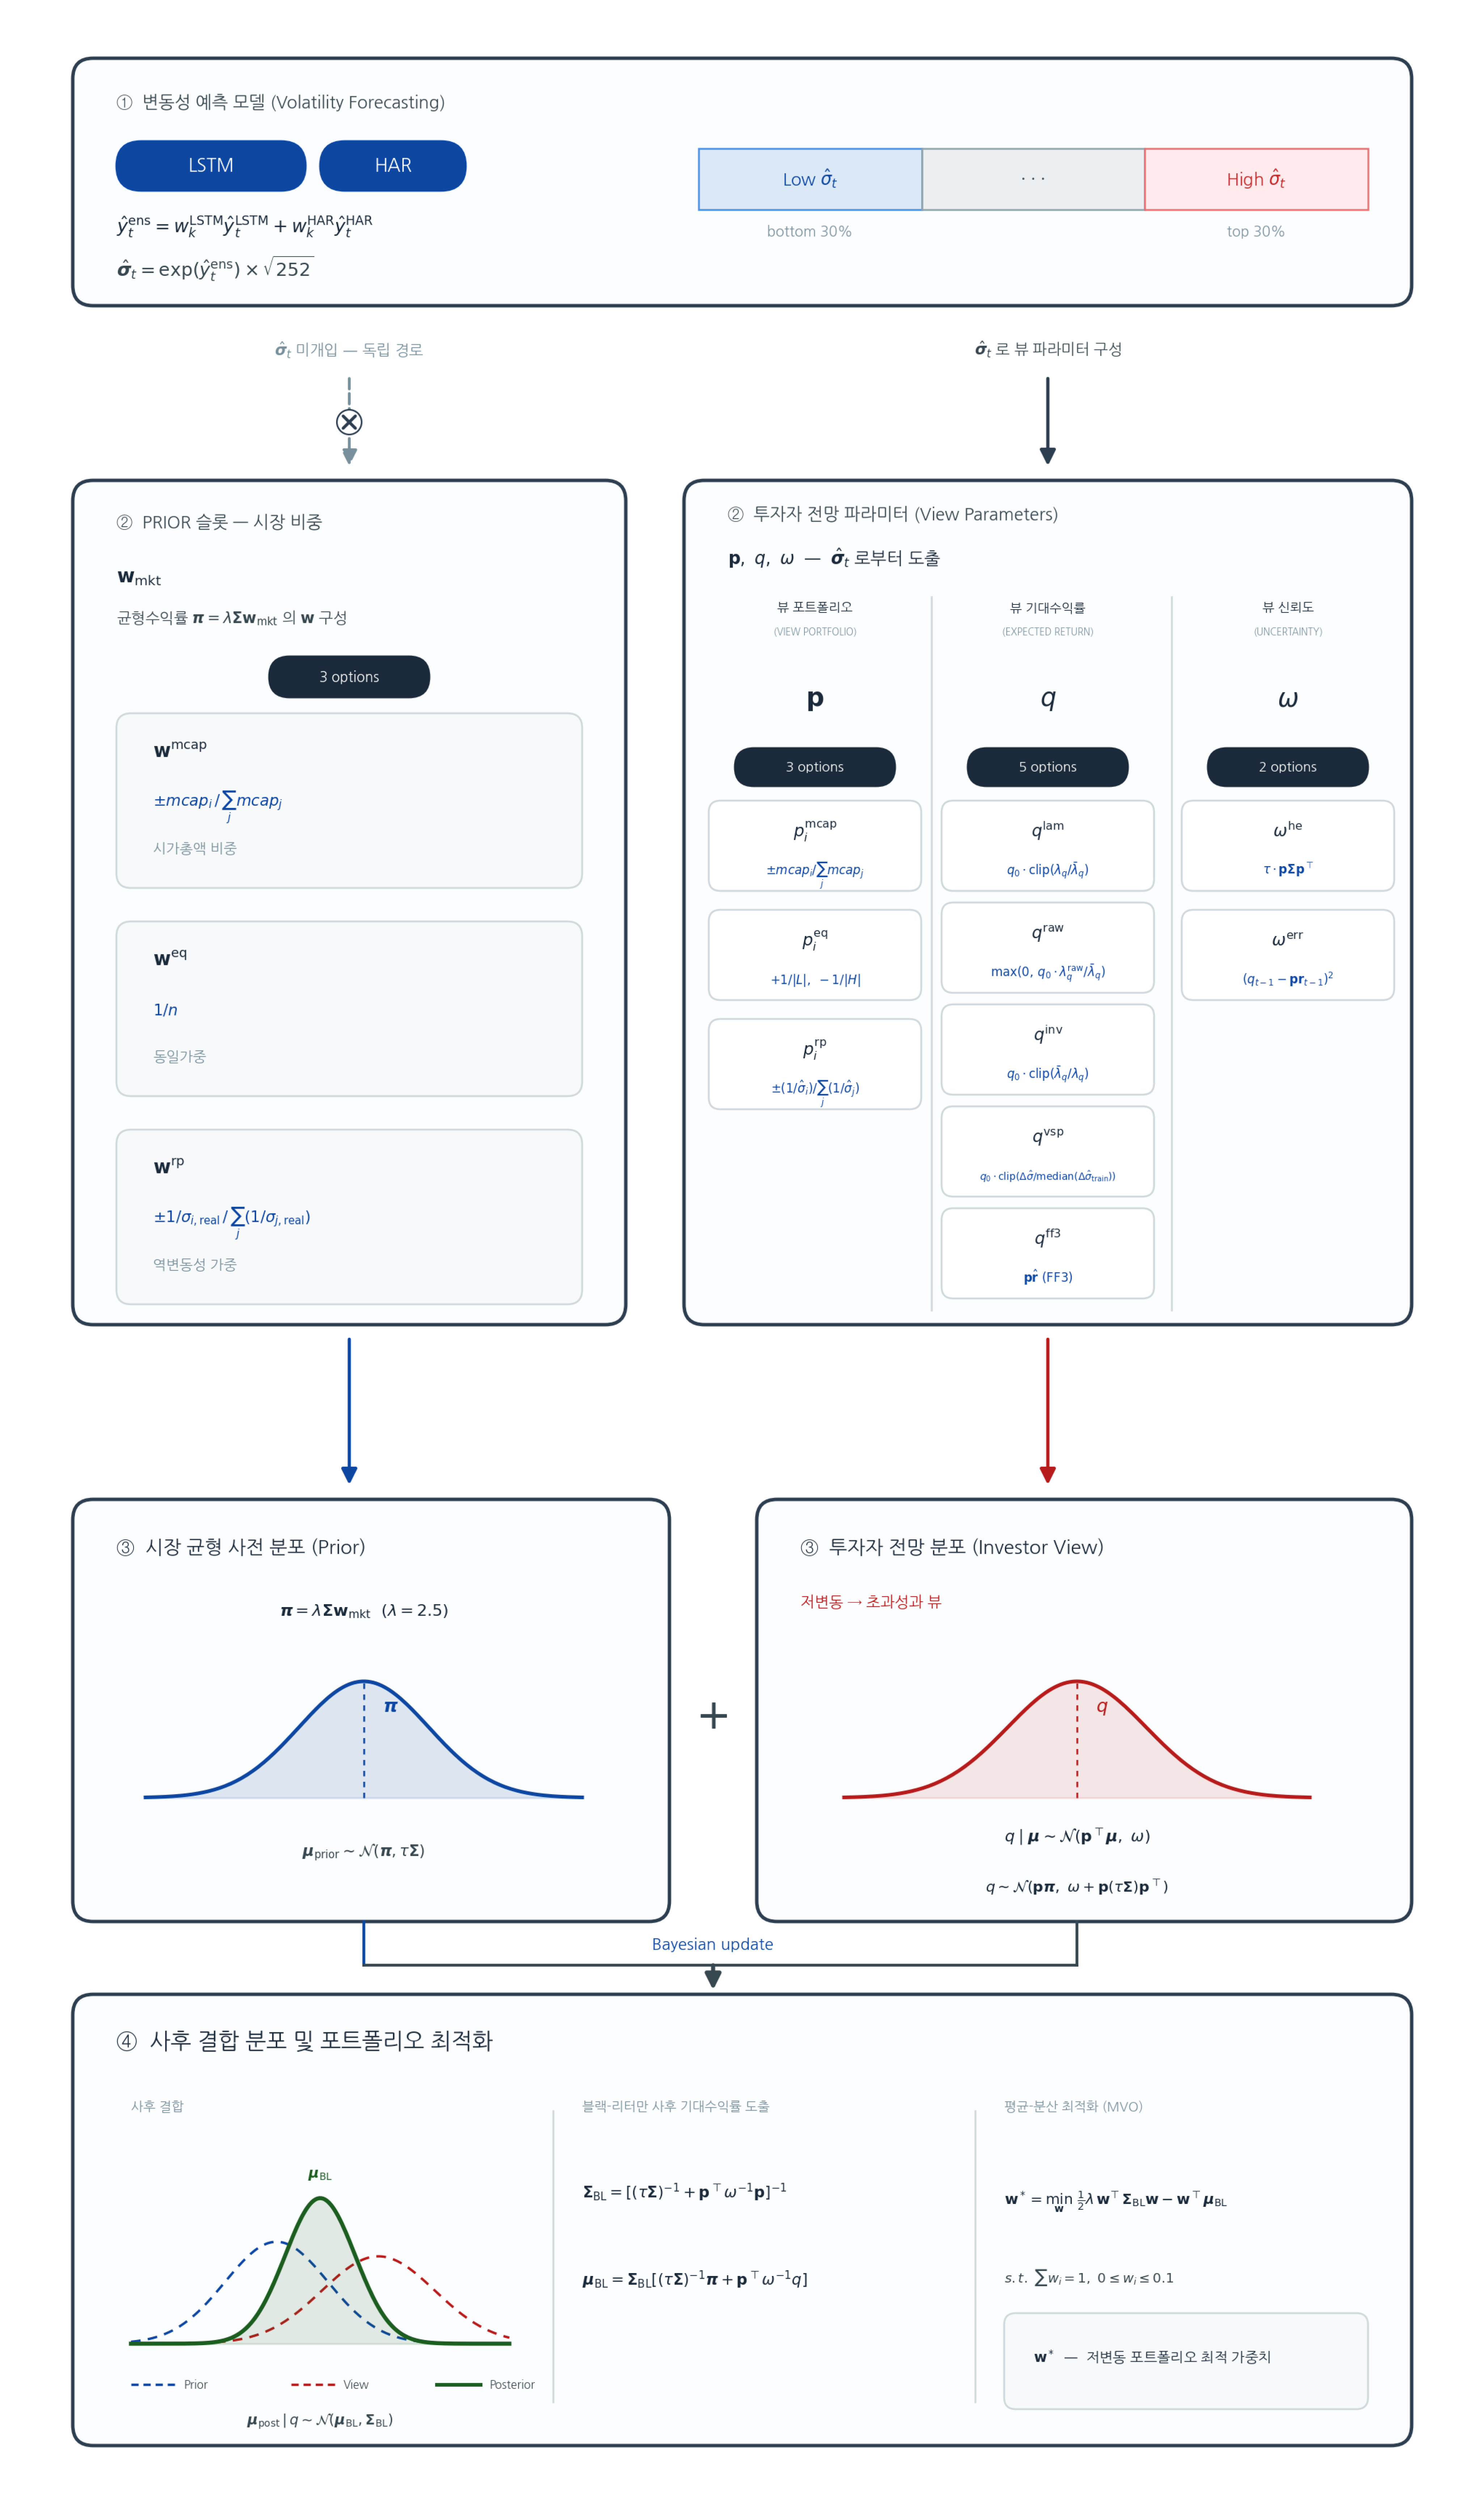
\includegraphics[height=0.85\textheight, keepaspectratio]{Figure/bl_pipeline.png}
    \caption{본 연구의 전체 분석 파이프라인.}
    \label{fig:pipeline}
\end{figure}

전체 연구 파이프라인은 그림~\ref{fig:pipeline}과 같이 네 단계로 구성된다. (1) LSTM-HAR 앙상블 모형으로 자산별 변동성 $\hat{\sigma}_t$를 예측한 후, 하위 및 상위 30\% 구간을 각각 저변동·고변동 종목으로 분류한다. (2) $\hat{\sigma}_t$는 BL 뷰 파라미터 ($\mathbf{p}, q, \omega$) 구성에 활용되며, 사전 분포 $\mathbf{w}_{mkt}$는 $\hat{\sigma}_t$와 독립적인 경로로 산출된다. 이때 네 슬롯은 각각 3·5·2·3개의 후보를 가지고 있어 총 90개 조합을 형성한다. (3) 시장 균형 사전 분포와 투자자 전망 분포를 베이지안 매커니즘으로 결합하여 (4) 사후 분포 $(\boldsymbol{\mu}_{BL}, \boldsymbol{\Sigma}_{BL})$를 도출하고, MVO를 통해 저변동 포트폴리오 최적 자산 배분 가중치 $\mathbf{w}^*$를 산출한다. 이어지는 절에서는 각 단계의 구체적인 방법론을 기술한다.

\subsection{변동성 예측}\label{subsec:vol_pred}

본 절에서는 앞서 \ref{subsec:vol_pred_review}절에서 살펴본 HAR 모형과 LSTM 모형, 그리고 이를 결합하는 예측 앙상블 방법론과 Walk-Forward 구조를 본 연구에 적용한 구체적인 구현 방식을 기술한다.

\subsubsection{종속변수와 입력변수}\label{subsubsec:variable}
본 연구는 시점 $t$ 기준 향후 21영업일 (약 1개월) 수익률의 표준편차를 종속변수로 사용한다. 21일 예측 윈도우(window) 길이는 포트폴리오 리밸런싱 주기(월 1회)와 일치하도록 동기화되며, 일별 로그 수익률 $r$을 이용하여 다음과 같이 정의된다.
\begin{equation}
y_t = \log\bigl(\mathrm{std}(r_{t+1}, \ldots, r_{t+21})\bigr)
\label{eq:vol_target}
\end{equation}
정의된 종속변수에는 로그 변환을 적용한다. 로그 변동성은 근사적으로 정규분포를 따르므로, MSE를 평가지표로 사용할 때 학습 안정성을 확보할 수 있다는 장점이 있다. 또한 로그 공간에서 학습하기 때문에 지수 역변환을 거친 후에도 항상 양수(positive) 예측이 보장된다. 모형 성능 평가에는 RMSE(Root Mean Squared Error)를 주된 지표로 사용하며, 보조 지표로 스피어만(Spearman) 상관계수와 Hit rate를 함께 확인하여 예측의 방향성과 순위 보존 능력을 종합적으로 평가한다.

입력변수는 1일·5일·22일 세 가지 시간 척도의 변동성 대리변수를 활용하며, 이는 일별 종가수익률 제곱으로 산출한다.
\begin{align}
RV_{d,t} &= r_t^2,\\
RV_{w,t} &= \frac{1}{5}\sum_{s=0}^{4} r_{t-s}^2,\\
RV_{m,t} &= \frac{1}{22}\sum_{s=0}^{21} r_{t-s}^2.
\end{align}
이는 \citet{corsi2009}의 원본 HAR 모형이 사용하는 일내 고빈도 실현변동성을 일별 종가 기반 대리변수로 근사한 형태이다. 본 연구의 분석 대상인 S\&P 500 종목군 (약 617 종, 2010--2025) 전반에 대해 일관된 일내 고빈도 데이터를 확보하기 어렵다는 현실적인 제약을 고려하여, 이와 같은 일별 종가 기반 근사를 채택하였다.

HAR 모형은 위 세 가지 항만을 입력으로 사용하는 반면, LSTM 모형은 세 항의 로그 변환 값에 추가로 시장의 미래 변동성 기대를 반영하는 변동성 지수 (CBOE Volatility Index, VIX, \citealp{whaley2009understanding})의 로그 변환 값을 포함하여 총 4 차원의 입력 벡터를 구성한다.
\begin{equation}
\mathbf{x}_t = \bigl[\log RV_{d,t},\ \log RV_{w,t},\ \log RV_{m,t},\
\log \text{VIX}_t\bigr]^\top
\label{eq:vol_input}
\end{equation}
LSTM 모형에 VIX 지수를 추가한 이유는 S\&P 500 옵션 시장에 내재된 미래 변동성 기대가 개별 종목의 향후 실현 변동성을 예측하는 데 유용한 정보를 제공할 것이라는 가정에 기반한다.

모형의 최종 출력값 $\hat{y}_t$는 식~(\ref{eq:vol_target})에 따라 일별 로그 변동성의 표준편차이다. BL의 시장 균형 수익률 $\boldsymbol{\pi}$와 공분산 행렬 $\boldsymbol{\Sigma}$가 모두 연환산 단위로 정의되므로, 변동성 예측 뷰 역시 동일한 단위로 맞추기 위해 지수 역변환 후 연환산 과정을 거친다.
\begin{equation}
\hat{\sigma}_t = \exp(\hat{y}_t) \times \sqrt{252}
\label{eq:bl_input}
\end{equation}
여기서 $\sqrt{252}$ 는 일간 표준편차를 연간 표준편차로 환산하는 처리이다.

\subsubsection{예측 모형}

본 절에서는 변동성 예측 모형으로 활용된 LSTM과 HAR, 그리고 두 모형의 앙상블 구조와 기준 모형인 ANN의 구체적인 구조 및 하이퍼파라미터 설정을 기술한다.

\paragraph{LSTM}
LSTM 모형은 \ref{subsubsec:lstm_review}절에서 살펴본 표준 LSTM 셀 구조(그림~\ref{fig:lstm_cell}, 식~\ref{eq:lstm_f}--\ref{eq:lstm_h})를 1개의 은닉층(1-layer), 은닉 노드 수 32개, 드롭아웃 비율 0.3, 그리고 시퀀스 길이는 63영업일로 구성한다. 시퀀스 길이를 63영업일로 설정한 것은 약 3개월의 시간 척도에 해당하는 기간으로, 변동성 대리변수인 S\&P 500 지수(SPY) 일별 수익률 제곱 시계열의 자기상관이 lag 60 전후까지 통계적으로 유의하게 지속됨을 EDA에서 확인한 결과에 근거한 선택이다. 개별 종목별로 자기상관 길이에 미세한 차이는 존재할 수 있으나, 모형의 통일성과 일관된 평가를 위해 전 종목에 동일하게 적용한다.

학습은 AdamW 옵티마이저(학습률 $10^{-3}$, 가중치 감쇠 $10^{-3}$), MSE 손실함수를 사용하며, 최대 50 에포크(epoch) 동안 진행된다. 이 과정에서 과적합을 방지하기 위해 10 에포크 동안 검증 손실(validation loss)이 개선되지 않을 경우 학습을 중단하는 조기 종료(early stopping) 규칙을 적용하며, 배치 크기(batch size)는 64로 설정한다. 입력 시퀀스 $\mathbf{X}_{t-L+1}, \ldots, \mathbf{X}_t$ ($L=63$) 에 대한 최종 로그 변동성 예측은 다음과 같다.
\begin{equation}
\hat{y}^{\text{LSTM}}_t = f_{\text{LSTM}}(\mathbf{X}_{t-L+1}, \ldots,
\mathbf{X}_t)
\label{eq:lstm_pred}
\end{equation}

\paragraph{HAR}
HAR 모형은 \ref{subsubsec:har_review}절의 식~\ref{eq:har_full}의 구조를 본 연구의 일별 변동성 대리변수에 적용한다. 회귀계수
$(\beta_0, \beta_d, \beta_w, \beta_m)$는 각 IS 구간에서 OLS(Ordinary Least Squares) 방식으로 추정하며, OOS 구간에 대한 예측값은 추정된 회귀계수와 OOS 입력 변수의 선형 결합으로 다음과 같이 산출한다.
\begin{equation}
\hat{y}^{\text{HAR}}_t = \beta_0 + \beta_d \log RV_{d,t} + \beta_w \log
RV_{w,t}+ \beta_m \log RV_{m,t}
\label{eq:har_pred_impl}
\end{equation}

\paragraph{Performance-Weighted 앙상블}
최종 변동성 예측값은 앞서 \ref{subsubsec:ens_review}절에서 제시한 performance-weighted 결합 방식(식~\ref{eq:perf_weight_general})을 LSTM과 HAR 두 모형에 적용하여 산출한다. 폴드(fold) $k$에서의 모형별 가중치는 직전 폴드 $k-1$의 OOS RMSE 역수에 비례하게 설계되었으며, 폴드 $k=0$에서는 사전 성능 정보가 없으므로 두 모형에 동일한 가중치 0.5를 부여한다.

\begin{align}
w_k^{\text{LSTM}} &= \frac{1/\text{RMSE}_{k-1}^{\text{LSTM}}}
{1/\text{RMSE}_{k-1}^{\text{LSTM}} + 1/\text{RMSE}_{k-1}^{\text{HAR}}},
\label{eq:ens_weight_lstm}\\
w_k^{\text{HAR}} &= 1 - w_k^{\text{LSTM}}.
\label{eq:ens_weight_har}
\end{align}

최종 앙상블 변동성 예측값은 두 모형의 가중 평균이다.

\begin{equation}
\hat{y}^{\text{ens}}_t = w_k^{\text{LSTM}} \cdot \hat{y}^{\text{LSTM}}_t
+ w_k^{\text{HAR}} \cdot \hat{y}^{\text{HAR}}_t
\label{eq:ens_pred}
\end{equation}

두 모형의 개별 예측 성능 및 앙상블 결합을 통한 오차 감소 효과는 추후 \ref{subsec:vol_pred_eval}에서 비교 분석한다. 그림 \ref{fig:ensemble_flow}은 입력 변수부터 최종 BL 입력치 산출까지의 전체 흐름을 요약한다.

\begin{figure}[t]
\centering
\renewcommand{\arraystretch}{1.4}
\begin{tabular}{c c c c c c c}
\textbf{입력} & & \textbf{모형} & & \textbf{가중 결합} & & \textbf{BL 입력} \\
\hline
$\log RV_{d,t}, \log RV_{w,t}, \log RV_{m,t}, \log \text{VIX}_{t}$ & $\longrightarrow$ & LSTM & $\searrow$ & & & \\
& & & & $\hat{y}^{\text{ens}}_t$& $\longrightarrow$ & $\hat{\sigma}_t$\\
$\log RV_{d,t}, \log RV_{w,t}, \log RV_{m,t}$ & $\longrightarrow$ & HAR & $\nearrow$ & & & \\
\end{tabular}
\caption{Performance-weighted 앙상블 기반의 변동성 예측 흐름.}
\label{fig:ensemble_flow}
\end{figure}

\paragraph{ANN (기준 모형)}
본 연구는 \ref{subsec:bl_vol_review}절의 \citet{pyo2018}의 ANN을 기준 모형으로 설정하여, 동일한 평가 환경 하에서 함께 평가한다. \citet{pyo2018}는 ANN의 세부 구조를 명시적으로 보고하지 않았으나, 금융 데이터 특성상 학습 표본 크기가 제한적이어서(60개월 윈도우 기준 유효 표본 약 50개) 과적합 위험이 크다는 점을 고려하였다. 이에 따라 학습 가능 파라미터 수(49개)가 학습 표본 수(약 50개)와 유사한 범위 내에 머물도록, 단일 은닉층 4개의 뉴런으로 구성된 소규모 구조로 재현하여 과적합 위험을 최소화하였다.(그림~\ref{fig:ann_arch}). 은닉층의 활성화 함수로는 ReLU를, 옵티마이저는 Adam을 사용하며, 과적합 방지를 위해 추가적으로 $L_2$ 정규화($\alpha = 0.01$)를 적용하여 추정의 안정성을 보완하였다.

\begin{figure}[t]
\centering
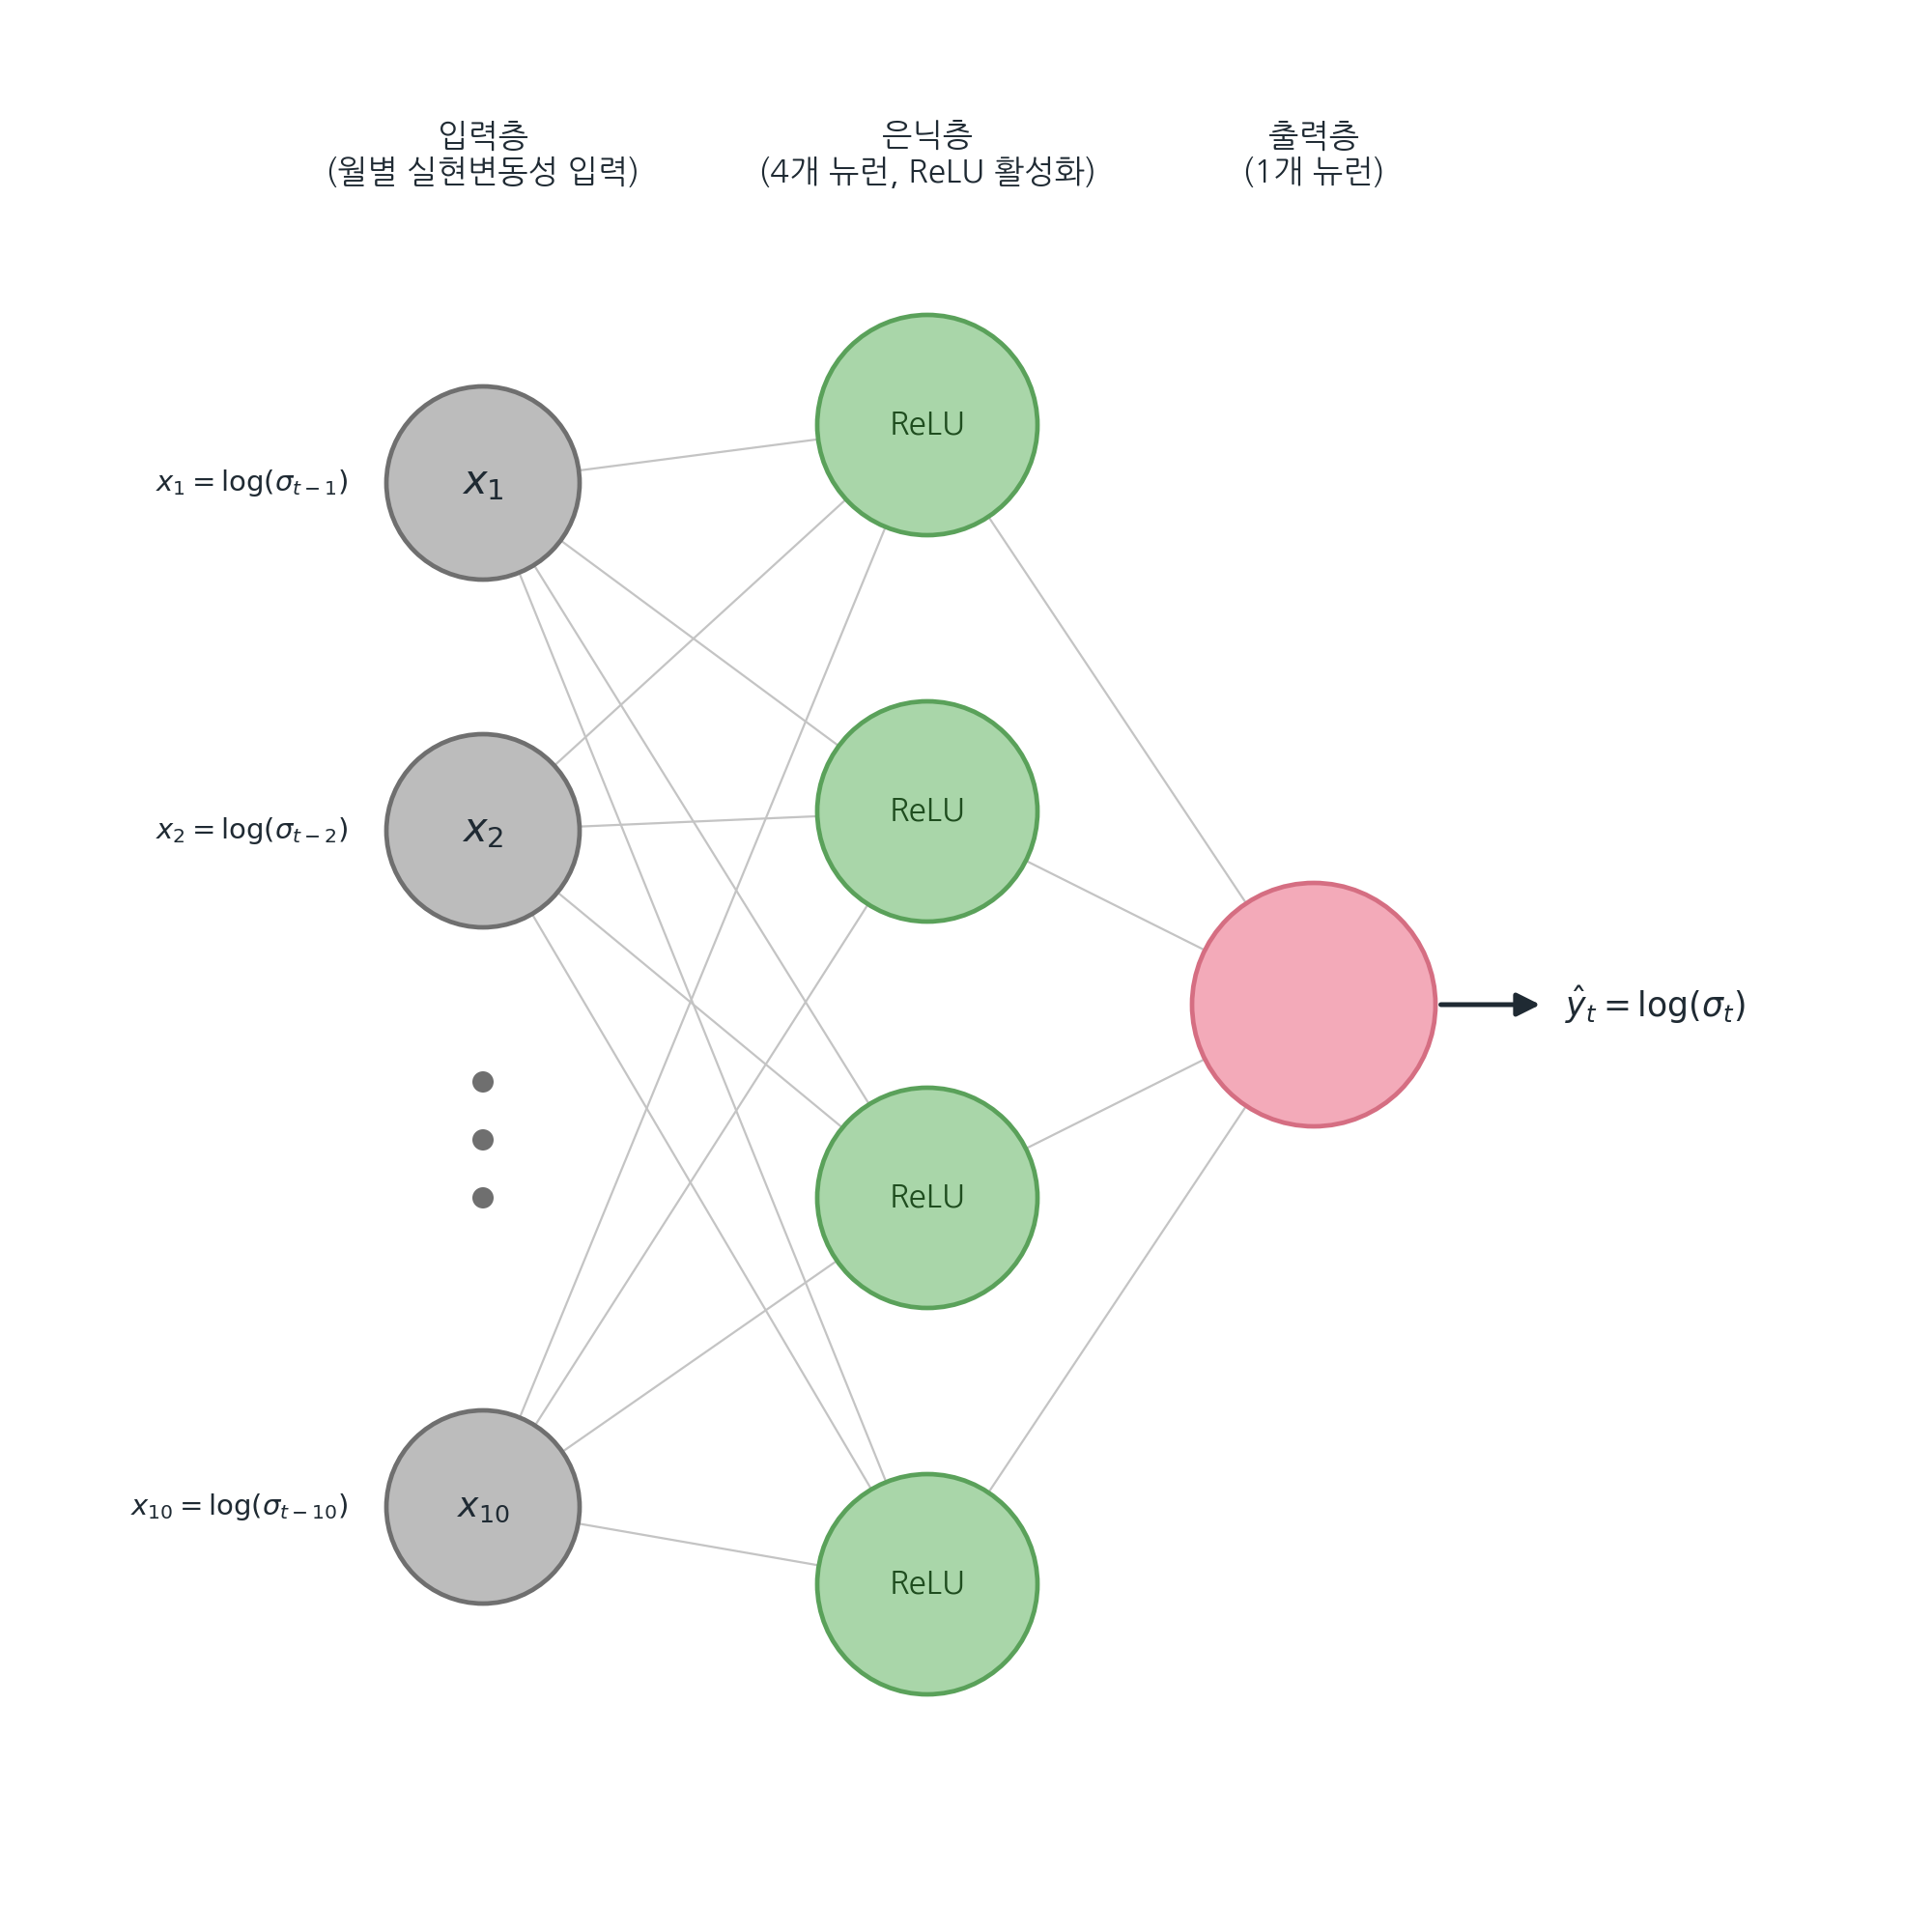
\includegraphics[width=0.7\textwidth]{Figure/ann_architecture.png}
\caption{ANN 기준 모형의 구조.}
\label{fig:ann_arch}
\end{figure}

\citet{pyo2018}의 원본 사양에 따라, ANN의 입력 변수는 직전 10개월의 월별 로그 변동성을, 출력 변수는 익월의 월별 로그 변동성을 사용한다. 각 월의 변동성은 해당 월말 기준 직전 21영업일 일별 수익률의 표준편차로 정의하여, LSTM 및 HAR 모형이 사용하는 향후 21영업일 변동성(식~\ref{eq:vol_target})과 동일한 일별 로그 변동성 단위로 산출되도록 하였다. 샘플링 주기(일별/월별)에 차이가 있으나 출력 단위가 동일하여 \ref{subsec:vol_pred_eval}절의 Walk-Forward 평가에서 직접 비교가 가능하다.

\subsubsection{Walk-Forward 학습·평가}

\ref{subsubsec:walk_forward_review}절의 퍼징-엠바고 Walk-Forward 구조를 모든 변동성 모형(LSTM, HAR, 앙상블, ANN)의 학습 및 평가에 동일하게 적용한다. 각 폴드는 그림~\ref{fig:walk_forward}과 같이 IS 1,250 영업일(약 5년), 퍼징 21영업일, 엠바고 63영업일, OOS 21영업일의 네 가지 구간으로 구성되며, 매 21영업일 간격으로 전진 이동(rolling)한다.

\begin{figure}[t]
\centering
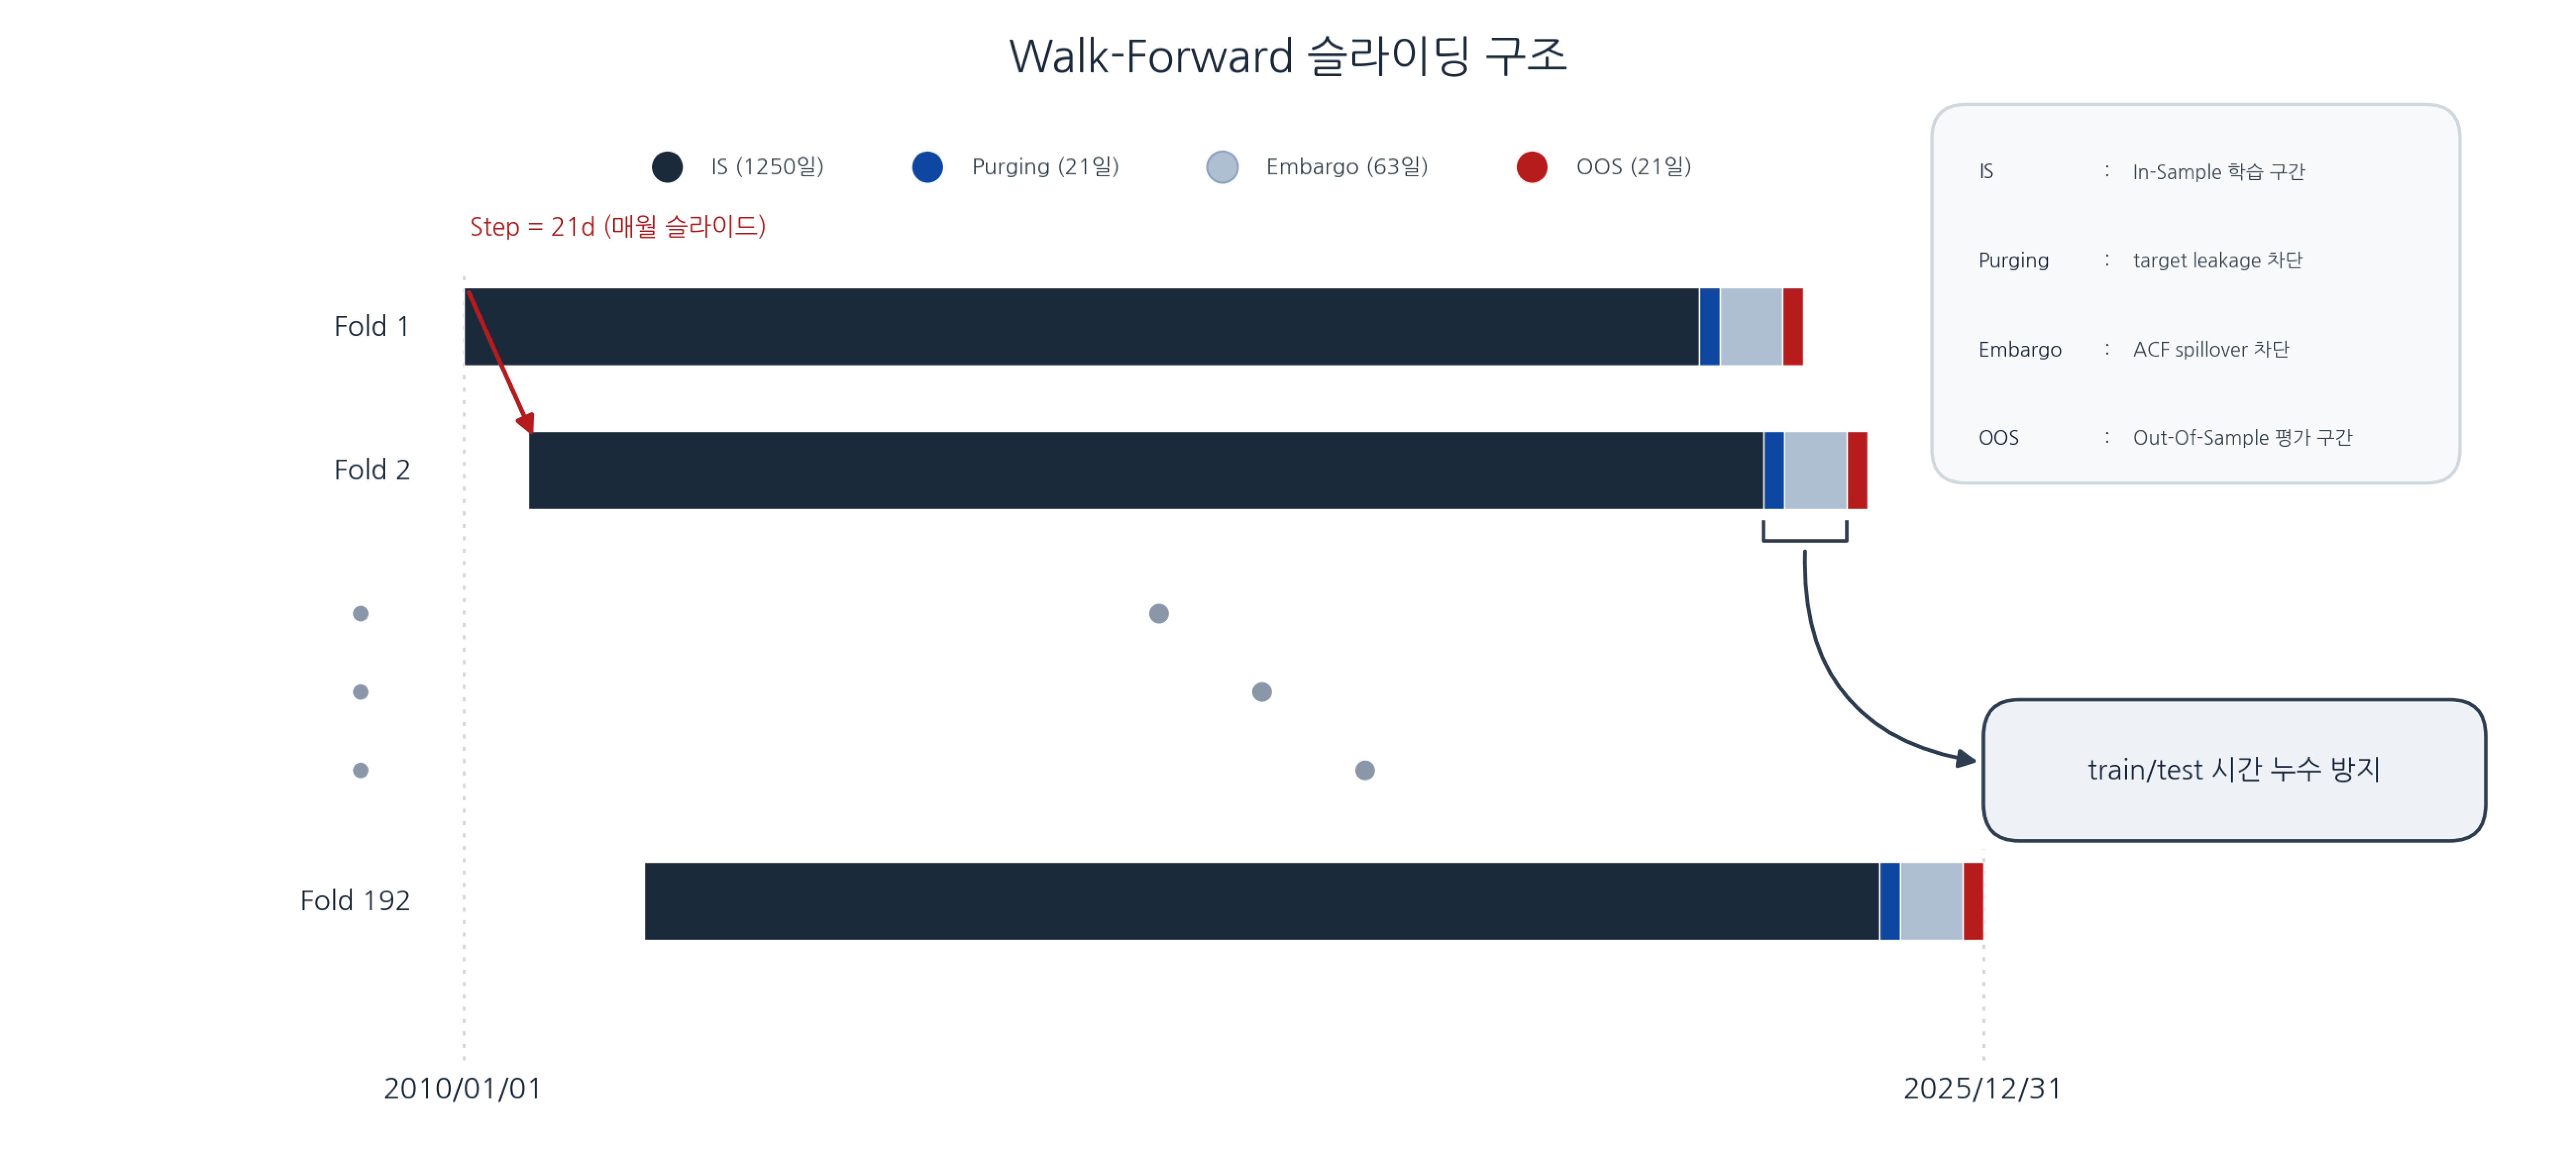
\includegraphics[width=0.95\textwidth]{Figure/walkforward.png}
\caption{Walk-Forward 슬라이딩 평가 구조 (IS 1{,}250 · Purging 21 · Embargo 63 · OOS 21 영업일).}
\label{fig:walk_forward}
\end{figure}

IS 구간의 1,250영업일은 \citet{pyo2018}의 학습 윈도우(60개월)와 동일한 조건 하에서 비교하기 위해 설정하였다. 퍼징 구간의 21영업일은 종속변수의 미래 예측 윈도우(식~\ref{eq:vol_target})와 동일한 길이로 설정되었으며, IS 마지막 시점의 미래 타깃이 OOS 구간과 시간적으로 중첩되지 않도록 차단한다. 엠바고 구간의 63영업일은 앞서 정의한 LSTM 모형의 입력 시퀀스 길이(63영업일)와 일치하도록 설정하여, 변동성 자기상관이 충분히 감쇠한 이후에 OOS 평가를 시작하도록 제한한다.

\subsection{블랙-리터만 구조 및 슬롯}\label{sec:bl}

본 절에서는 앞서 \ref{subsec:bl_review}절의 BL 일반식(식 \ref{eq:bl_pi}--\ref{eq:bl_w})에 등장하는 네 가지 입력 변수인 $\mathbf{w}_{mkt}$ (사전 분포), $\mathbf{p}$ (뷰 포트폴리오), $q$ (뷰 기대수익률), $\omega$ (뷰 신뢰도) 각각에 대해 본 연구에서 비교$\cdot$분석할 슬롯별 옵션을 정의한다. \ref{subsec:bl_vol_review}절의 \citet{pyo2018}가 각 입력 변수에 단일 설정을 채택한 반면, 본 연구는 \ref{subsec:vol_pred}절의 변동성 예측 결과를 BL 구조에 어떻게 연결할지에 따라 각 입력을 옵션 집합으로 일반화하고, 그 곱집합(Cartesian product)을 슬롯 그리드로 정의한다.

\subsubsection{제안 슬롯}\label{subsubsec:bl_proposed_slot}

\paragraph{사전 분포 ($\mathbf{w}_{mkt}$)}

균형 수익률 $\boldsymbol{\pi}$(식~\ref{eq:bl_pi}) 계산에 사용하는 시장 비중 $\mathbf{w}_{mkt}$를 세 가지 방식으로 구성한다.

\begin{itemize}
    \item $\mathbf{w}^{\mathrm{mcap}}$: 시가총액 비중 가중. \citet{pyo2018}의 원안이며, CAPM의 균형 시장 포트폴리오 가정에 부합한다.
    \item $\mathbf{w}^{\mathrm{eq}}$: 동일 가중. 유니버스 전체에 균등한 사전 정보를 부여한다.
    \item $\mathbf{w}^{\mathrm{rp}}$: 직전 21영업일 실현 변동성의 역수($1/\sigma_{\mathrm{realized}}$) 비중 가중. 저변동 종목에 더 큰 가중치를 배분하는 리스크 패리티\citep{maillard2010} 철학에 기반한다. 단, 사용하는 변동성은 LSTM 예측값이 아닌 전월의 실현 변동성이다.
\end{itemize}

\paragraph{뷰 포트폴리오 ($\mathbf{p}$)}

$\mathbf{p}$ 벡터는 저변동 자산이 고변동 자산을 초과 성과할 것이라는 뷰를 인코딩한다. 각 리밸런싱 시점 $t$에서 유니버스 내 종목을 앙상블 예측 변동성 $\hat{\sigma}_{i,t}$ 기준으로 오름차순 정렬 후, 하위 30\%(저변동 그룹 $L$)에 양($+$)의 가중치, 상위 30\%(고변동 그룹 $H$)에 음($-$)의 가중치를 부여하며, 나머지 40\%는 0으로 처리한다. 롱 측 가중치의 합은 $+1$, 숏 측 가중치의 합은 $-1$로 정규화되어 $\sum_i p_i = 0$을 만족하며, 이는 자기자금조달(self-financing) 롱-숏 포트폴리오 뷰에 해당한다. 분류 임계값(상하위 30\%)은 \citet{pyo2018}의 설정을 따르며, 그룹 내 가중 방식은 본 연구에서 세 가지로 일반화한다.

\begin{itemize}
  \item $\mathbf{p}^{\mathrm{mcap}}$: 시가총액 비례 가중. \citet{pyo2018}의 원안으로, 각 그룹 내 시가총액 합계로 정규화한다. 식은 \eqref{eq:pyo_p}와 동일한 표현이다.

  \item $\mathbf{p}^{\mathrm{eq}}$: 동일 가중. 각 그룹 내 모든 종목에 $+1/|L|$ (롱 측) 또는 $-1/|H|$ (숏 측) 을 배분하여, 시가총액 집중에 따른 편향을 제거하고 변동성 분류 신호를 균등하게 반영한다.

  \item $\mathbf{p}^{\mathrm{rp}}$: 역변동성 가중. 그룹 내 종목에 예측 변동성의 역수에 비례한 비중을 배분한다.
    \begin{equation}
      p_i^{\mathrm{rp}} =
      \begin{cases}
        +\dfrac{1/\hat{\sigma}_i}{\sum_{j \in \mathcal{L}} 1/\hat{\sigma}_j}, & i \in \mathcal{L}, \\[8pt]
        -\dfrac{1/\hat{\sigma}_i}{\sum_{j \in \mathcal{H}} 1/\hat{\sigma}_j}, & i \in \mathcal{H}, \\[6pt]
        \phantom{+}0, & \text{otherwise}.
      \end{cases}
      \label{eq:p_rp}
    \end{equation}
    분류(상하위 30\% 선택) 단계에서는 모형 예측값의 순위 정보를, 가중(그룹 내 배분) 단계에서는 크기 정보를 각각 활용한다는 점에서, $\mathbf{p}^{\mathrm{rp}}$는 모형의 예측값이 이중으로 활용되는 구조다. 이러한 구조는 변동성 예측 신호를 포트폴리오에 적극적으로 반영할 수 있다는 한편, 모델의 추정오차가 누적될 위험을 수반한다. 
    %본 연구는 이를 사후적으로 통제하기 위해, 후술할 뷰 신뢰도($\omega$) 슬롯에서 통해 뷰의 불확실성을 동적으로 조정함으로써 모델의 강건성을 보완한다.
\end{itemize}

\paragraph{뷰 기대수익률 ($q$)}

$q$는 저변동-고변동 그룹 간 기대수익률 스프레드로, 본 연구는 다섯 가지 슬롯을 비교한다. 다섯 가지 슬롯은 $q$를 결정하는 정보 채널에 따라 다음 세 범주로 구분된다.

\begin{itemize}
  \item \textbf{시장 위험회피도 ($\lambda_q$) 기반}: $q^{\mathrm{lam}}, q^{\mathrm{raw}}, q^{\mathrm{inv}}$ --- SPY 초과수익과 시장 분산으로 추정한 매크로 위험회피도를 신호로 사용한다.
  \item \textbf{예측 변동성 ($\Delta\hat{\sigma}$) 기반}: $q^{\mathrm{vsp}}$ --- 고/저변동 그룹의 예측 변동성 격차를 $q$에 직접 반영한다.
  \item \textbf{Fama-French 3팩터 모형 (FF3) 기반}: $q^{\mathrm{ff3}}$ --- \citet{pyo2018}의 원안에 해당하는 본 연구의 앵커 슬롯이다.
\end{itemize}

앞의 두 범주에 속하는 4개의 슬롯은 공통 기준값 $q_0 = 0.003$을 시장 신호로 동적 조정하는 반면, $q^{\mathrm{ff3}}$은 종목별 팩터 회귀 결과를 $\mathbf{p}$ 벡터와 결합하여 $q$를 직접 산출한다.

\textbf{기준값 $q_0$ 설정.} 4개 동적 조정 슬롯의 기준값 $q_0 = 0.003$(월 0.3\%)은 저위험 이상현상 실증 문헌의 보고치를 보수적으로 반영한 값이다. \citet{frazzini2014}는 미국 주식 표본에서 BAB(Betting Against Beta) 팩터의 월 평균 초과수익을 약 0.55--0.70\% 수준으로 보고하며, \citet{baker2011}, \citet{blitz2007} 역시 저변동 long-short 전략의 월 수익이 0.4--0.7\% 범위임을 확인한다. 본 연구는 예측 모형의 오판 가능성을 감안해 실증치의 약 절반인 0.3\%를 기준값으로 채택한다.

\textbf{$\lambda_q$ 기반 슬롯.} 동적 조정에 사용하는 시장 위험회피도 $\lambda_q$는 $\boldsymbol{\pi}$ 계산용 고정 $\lambda = 2.5$와 별개로, 매 시점 다음과 같이 추정한다.
\begin{equation}
  \lambda_q = \mathrm{clip}\!\left(\bar{r}^{\mathrm{ex}}_{\mathrm{SPY}}/\sigma^2_{\mathrm{mkt}},\ 0.5,\ 10.0\right),
\end{equation}
여기서 $\mathrm{clip}(x, a, b) = \min(\max(x, a), b)$는 $x$의 값을 $[a, b]$ 범위로 상·하한을 제한하는 함수이며, $\bar{r}^{\mathrm{ex}}_{\mathrm{SPY}}$는 SPY 평균 초과수익률, $\sigma^2_{\mathrm{mkt}}$는 시장 수익률 분산, $\bar{\lambda}_q$는 훈련 기간 내 $\lambda_q$의 평균이다.

\begin{itemize}
  \item $q^{\mathrm{lam}}$: $\lambda_q$ 비례 조정. 시장이 안정적($\lambda_q$ 상승)일수록 $q$를 강화하고, 불안정($\lambda_q$ 하락)할수록 약화한다.
    \begin{equation}
      q^{\mathrm{lam}} = q_0 \times \mathrm{clip}\!\left(\lambda_q/\bar{\lambda}_q,\ 0.1,\ 3.0\right).
    \end{equation}
    $[0.1, 3.0]$ 범위의 상·하한 제약은 $q$가 $q_0$의 10\% 미만으로 소멸하거나 3배를 초과하여 증폭되는 것을 방지하기 위한 실용적 제약이며, $q^{\mathrm{inv}}$와 $q^{\mathrm{vsp}}$에도 동일하게 적용된다.

  \item $q^{\mathrm{raw}}$: 상·하한 제약 적용 이전의 $\lambda_q$ 사용. SPY 하락으로 $\lambda_q^{\mathrm{raw}} < 0$이면 $q$가 0으로 수렴하여, 시장 방향에 따라 뷰가 자연 소멸된다.
    \begin{equation}
      q^{\mathrm{raw}} = \max\!\left(0,\ q_0\times \lambda_q^{\mathrm{raw}}/\bar{\lambda}_q\right).
    \end{equation}

  \item $q^{\mathrm{inv}}$: $\lambda_q$ 역수 조정. 불안정 국면에서 $q$를 강화하여 저변동 방어 전략을 키우는, $q^{\mathrm{lam}}$과 반대 방향으로 작동한다.
    \begin{equation}
      q^{\mathrm{inv}} = q_0 \times \mathrm{clip}\!\left(\bar{\lambda}_q/\lambda_q,\ 0.1,\ 3.0\right).
    \end{equation}
\end{itemize}

\textbf{예측 변동성 기반 슬롯.} $q^{\mathrm{vsp}}$는 모형의 예측 변동성 격차를 훈련 기간 중앙값으로 정규화하여 $q$의 크기를 조정한다. $\lambda_q$ 분류가 매크로 시장 신호를 사용하는 반면, $q^{\mathrm{vsp}}$는 LSTM 예측 변동성을 $q$에 직접 반영한다.
\begin{equation}
  q^{\mathrm{vsp}} = q_0 \times \mathrm{clip}\!\left(\Delta\hat{\sigma}_t/\mathrm{median}(\Delta\hat{\sigma}_{\mathrm{train}}),\ 0.1,\ 3.0\right),
\end{equation}
여기서 $\Delta\hat{\sigma}_t = \frac{1}{|H|}\sum_{i\in H}\hat{\sigma}_{i,t} - \frac{1}{|L|}\sum_{i\in L}\hat{\sigma}_{i,t}$이며, $H, L$의 정의에 의해 $\Delta\hat{\sigma}_t > 0$이 보장된다. 이 값은 매 리밸런싱 시점마다 시장 상황에 따라 크게 달라질 수 있어, 훈련 기간 내 $\Delta\hat{\sigma}_t$ 시계열의 중앙값으로 나누어 정규화함으로써 위기 구간 등 극단적으로 커지는 시점이 기준값에 미치는 영향을 억제하였다.

\textbf{팩터 모형 기반 슬롯.} \citet{pyo2018}는 FF3 회귀로 $q$를 산출한다는 방향만 제시하고 팩터 프리미엄 산정 방식의 세부는 명시하지 않아, 본 연구는 단기 추정의 불안정성을 피하기 위해 훈련 윈도우(60개월) 내 팩터 평균을 다음 달 기대 팩터 프리미엄으로 사용하는 방식 \citep{fama1973risk, cochrane2005} 으로 구현하였다. 종목별 FF3 롤링 회귀로 추정한 기대수익률 $\hat{r}_i$와 $\mathbf{p}$ 벡터의 결합으로 $q$를 산출하며, 훈련 기간 내 데이터만 사용하므로 look-ahead bias가 없다. 이 구현이 \citet{pyo2018}의 FF3 방식에 해당하는 본 연구의 앵커 슬롯이다.
\begin{equation}
  q^{\mathrm{ff3}} = \mathbf{p}\hat{\mathbf{r}}, \qquad
  \hat{r}_i = \hat{\alpha}_i + \hat{\beta}_i^{\mathrm{mkt}}\bar{f}_{\mathrm{mkt}} + \hat{\beta}_i^{\mathrm{SMB}}\bar{f}_{\mathrm{SMB}} + \hat{\beta}_i^{\mathrm{HML}}\bar{f}_{\mathrm{HML}},
\end{equation}
여기서 $\bar{f}_k$는 훈련 윈도우 내 팩터 $k$의 평균값이며, SMB(Small Minus Big)와 HML(High Minus Low)은 FF3 표준 팩터다.

\paragraph{뷰 신뢰도 ($\omega$)}

$\omega$는 사전 균형 수익률 대비 투자자 뷰의 신뢰도를 결정하며, 본 연구는 다음 두 가지 설정을 비교한다.

\begin{itemize}
  \item $\omega^{\mathrm{he}}$ (He-Litterman 방식): 뷰 포트폴리오의 사전 분산에 비례하여 불확실성을 설정하는 BL 문헌의 표준 방식이다 \citep{helitterman1999}.
    \begin{equation}
      \omega^{\mathrm{he}} = \tau\mathbf{p}\boldsymbol{\Sigma}\mathbf{p}^\top.
    \end{equation}

  \item $\omega^{\mathrm{err}}$ (전월 예측 오차 기반): 각 시점 $t$에서 전월 ($t-1$)의 뷰 포트폴리오 예측 수익률과 실현 수익률 간 오차 제곱으로 불확실성을 추정하며, \citet{pyo2018}의 방식을 따른다.
    \begin{equation}
      \omega^{\mathrm{err}} = \left(q_{t-1} - \mathbf{p}_{t-1}\mathbf{r}_{t-1}\right)^2,
    \end{equation}
    여기서 $\mathbf{r}_{t-1}$은 $t-1$ 시점의 실현 수익률 벡터다. 전월 뷰 예측이 크게 빗나간 시점에서 불확실성이 자동으로 증가하는 자기교정적 구조이며, 첫 달은 $\omega^{\mathrm{he}}$로 초기화한다.

    이 구현은 \citet{pyo2018} 가 제시한 일반형 식 \eqref{eq:pyo_omega} 의 한 가지 해석에 해당한다. 원 식 $\omega = \mathrm{var}(\mathbf{P}_{t-1}\hat{\boldsymbol{\mu}}_{t-1} - \mathbf{P}_{t-1}\boldsymbol{\mu}_{t-1})$은 모두 단일 시점 $t-1$로 평가되어 있어, $\mathrm{var}$이 (i) $t-1$까지의 과거 시계열에 대한 표본분산인지, (ii) 단일 시점의 제곱 편차인지, (iii) 종목 단면 분산인지가 수학적으로 명확히 규정되지 않는 모호성이 존재한다. 본 연구는 BL 산출의 단순성과 직관성을 확보하기 위해 (ii) 의 해석을 채택하였다. 결과적으로 $\omega^{\mathrm{err}}$ 는 엄밀한 분산 추정량이 아닌 직전 시점 제곱 오차 추정치이나, 전월 오차 크기에 비례해 뷰 신뢰도가 자동 조정되는 자기교정 효과는 동일하게 보존된다.
\end{itemize}

\subsubsection{Walk-Forward 및 최적화}
\label{subsubsec:bl_walkforward}

포트폴리오 비중은 월별 리밸런싱 시점마다 시간 순서를 따라 산출하는 Walk-Forward 슬라이딩 방식으로 추정한다. 변동성 예측 단계(\ref{subsec:vol_pred}절)와 달리 현재 시점의 가중치를 산출하므로, 별도의 퍼징·엠바고 구간 없이, 매 리밸런싱 시점에서 직전 60개월 데이터를 사용한다. 각 리밸런싱 시점 $t$(월 1회)에서 다음 절차를 수행한다.

\begin{enumerate}
  \item 직전 60개월 일별 로그 수익률에 Ledoit-Wolf 수축 추정량 \citep{ledoitwolf2004}을 적용하여 공분산 행렬 $\boldsymbol{\Sigma}_t$를 산출한다. 이는 BL 프레임워크의 사전·사후 분포 계산에 사용되며, 변동성 예측 모형의 출력($\hat{\sigma}_{i,t}$)과는 독립적으로 산출된다.
  \item 해당 시점의 시장 비중 $\mathbf{w}_{mkt,t}$와 고정 위험회피도 $\lambda = 2.5$로 식 \eqref{eq:bl_pi}에 따라 균형 수익률 $\boldsymbol{\pi}_t$를 계산한다.
  \item 앙상블 모형(또는 ANN 기준 모형)의 예측 변동성 $\hat{\sigma}_{i,t}$로 $\mathbf{p}_t$를 구성하고, 슬롯 설정에 따라 $q_t$와 $\omega_t$를 산출한다.
  \item 식 \eqref{eq:bl_sigma_pos}, \eqref{eq:bl_mu_pos}에 따라 BL 사후 분포의 평균 $\boldsymbol{\mu}_{BL,t}$와 공분산 $\boldsymbol{\Sigma}_{BL,t}$를 계산한다.
  \item 식 \eqref{eq:bl_w}에 단일 종목 비중 상한 $w_i \leq 0.10$ 제약을 추가한 형태로 최적화하여 포트폴리오 비중을 산출한다.
\end{enumerate}

비중 상한 10\%는 극단적 집중 투자를 방지하기 위한 운용상 제약이다. 또한 데이터의 가용성을 확보하기 위해 각 리밸런싱 시점에서 훈련 윈도우(60개월) 내 일별 수익률 데이터가 90\% 이상 존재하는 종목만 유효 유니버스로 선별한다. 거래비용은 편측 20bp를 적용하며, 월별 실제 비중 변화량 $\sum_i |\Delta w_{i,t}|$에 비례하여 차감한다. 이는 S\&P 500 구성 종목의 실제 매매 스프레드 대비 보수적인 설정으로, $\omega^{\mathrm{err}}$ 슬롯의 예측오차 기반 신뢰도 조정이 고변동 구간에서 회전율을 높일 수 있다는 점을 고려한 것이다. 무위험 수익률은 미국 3개월 국채 수익률을 사용하며, 샤프 비율 산출 시 초과수익률 계산에 적용한다.

\subsubsection{평가 방법론}
\label{subsubsec:bl_eval}

전체 분석 기간은 2010년 1월부터 2025년 12월까지(192개월)이며, 시장 국면에 따라 성과가 크게 달라질 수 있으므로 전체 기간 평가와 국면별 성과 분해를 병행한다.

구체적인 국면 분류 과정은 \ref{app:hmm}에 상세히 기술되어 있으며, 본 연구는 Hidden Markov Model(HMM, \citealp{hamilton1989new}) 기반의 통계적 구조전환점 탐지와 금융 이벤트 도메인 지식을 결합하여 네 개의 비중첩 구간을 식별하였다(표 \ref{tab:regimes}).

각 국면 및 전체 기간에 대한 성과지표로는 샤프 비율, Sortino 비율, 최대 낙폭(Maximum Drawdown, MDD)을 산출한다. 이와 같은 국면별 성과 분해를 통해 앙상블 기반 BL 포트폴리오의 ANN 대비 우위가 특정 시장 국면에 의존하는지, 혹은 전 국면에 걸쳐 일관되게 유지되는지를 체계적으로 검증한다. 이를 위해 앙상블 모형과 ANN 기준 모형은 동일한 90개 슬롯 조합에 대해 1:1 대응 비교하며, 슬롯 구성은 두 모형 간 완전히 동일하게 유지한다.

\begin{table}[t]
\centering
\caption{분석 국면(regime) 구분 및 시기별 특성}
\label{tab:regimes}
\begin{tabular}{llcl}
\toprule
국면 & 기간 & 기간(개월) & 특성 \\
\midrule
R1 (회복기)  & 2010.01--2012.06 & 30 & Post-GFC 회복, 유럽 재정위기 \\
R2 (확장기)  & 2012.07--2019.12 & 90 & 장기 Bull Market, 저변동 \\
R3 (위기기)  & 2020.01--2023.06 & 42 & COVID-19, 2022 약세장 \\
R4 (정상화)  & 2023.07--2025.12 & 30 & AI 주도 랠리 \\
\midrule
\multicolumn{1}{l}{전체} & 2010.01--2025.12 & 192 & --- \\
\bottomrule
\end{tabular}
\end{table}



\section{실증 분석}\label{sec:result}

본 연구의 실증 분석은 2010년 1월부터 2025년 12월까지 총 16년(192개월) 동안 미국 S\&P 500 지수에 편입된 종목을 대상으로 수행한다. 종목 유니버스는 분석 기간 중 한 번이라도 S\&P 500에 포함되었던 833개 종목에서 출발하였다. 이 중 야후 파이낸스(Yahoo Finance)를 통해 일별 가격 데이터 확보가 가능한 617개 종목을 최종 분석 대상으로 선정하였으며, 데이터가 제외된 종목들은 상장 폐지나 인수합병 등으로 인한 가용성의 한계에 기인한다. 특히 매 리밸런싱 시점마다 해당 시점의 실제 S\&P 500 편입 종목만을 포트폴리오에 포함시키는 시점별 멤버십 필터링을 적용함으로써 생존 편향을 완화하였으나, 데이터 가용성 한계로 인한 편향을 완전히 배제할 수 없다. 그 외 결측치 처리, 거래비용, 자산별 비중 상한 등 구체적인 포트폴리오 운용 조건은 \ref{subsubsec:bl_walkforward}절에서 기술한 바와 같다.

분석에 사용된 주가, 시가총액, VIX 지수, 무위험 수익률 데이터는 야후 파이낸스에서 수집하였으며, FF3 시계열 데이터는 케네스 프렌치(Kenneth French) 데이터 라이브러리를 활용하였다. 또한, 시점별 S\&P 500 편입 종목 정보는 위키피디아(Wikipedia)의 S\&P 500 변경 이력을 바탕으로 구축하였다. 본 절은 변동성 예측 성능(\ref{subsec:vol_pred_eval}절), 기준 슬롯의 1차원 변형(\ref{subsec:baseline_slot}절), 슬롯 차원별 주변 분포(\ref{subsec:slot_config}절), 외부 벤치마크 대비 성과(\ref{subsec:benchmark}절) 순으로 실증 분석 결과를 제시한다.

\subsection{변동성 예측 성능}\label{subsec:vol_pred_eval}

표~\ref{tab:sigma_pred}는 LSTM 모형과 HAR 모형, 두 모형의 앙상블, 그리고 ANN 기준 모형의 변동성 예측 성능을 전체 기간과 4개 국면 구간 별로 비교한 결과이다.

먼저 단독 모형 성능을 보면, LSTM과 HAR 모형 모두 ANN 기준 모형 대비 일관된 우위를 보여 두 모형의 유용성을 확인하였다. 다만, 두 모형 간의 직접 비교에서는 지표에 따라 차별적인 강점이 관찰된다. LSTM 모형은 금융위기 구간인 R3 국면에서 Spearman 순위상관계수 우위(0.6772 vs HAR 0.6031)를 보이며 종목 간 상대적 변동성 순위를 우수하게 포착하였다. HAR 모형은 전 구간에 걸쳐 RMSE와 Hit Rate 측면에서 보다 안정적인 성능을 기록하였으며, 특히 R3 구간에서의 RMSE 격차(0.4336 vs LSTM 0.5064)가 두드러졌다. 이는 변동성이 급변하는 구간에서 LSTM 모형의 복잡한 학습 구조가 비정상적 패턴에 과적합되어 변동성 예측 오차를 확산시킨 반면, HAR 모형의 단순한 선형 구조는 짧은 표본에서도 안정적인 성능을 유지함을 시사한다. 

이처럼 두 단독 모형이 상이한 오차 특성을 지닌다는 점은, 모형 결합 시 결합 오차의 분산 감소 효과를 기대할 수 있다는 논리적 배경이 된다. 실제로 앙상블 모형은 이러한 상호 보완성을 효과적으로 활용하여 두 단독 모형의 성과를 모두 상회하였으며, 분석 대상인 총 20개의 셀(4개 평가지표 $\times$ 5개 분석 기간) 전반에서 가장 좋은 성능을 보인다. 이는 서로 다른 가정과 구조에 기반한 모형 결합이 단일 모형 대비 안정적인 예측력을 제공한다는 이론적 기대(\ref{subsubsec:ens_review})와 궤를 같이 한다.

특히 앙상블 모형과 ANN 기준 모형 간의 성과 격차는 R3 국면에서 가장 극명하게 나타났다. Spearman 순위상관 격차가 +0.310 (앙상블 0.6874 vs ANN 0.3771)로 가장 유의미한 향상을 보였는데, 이는 제안한 앙상블 모형이 시장의 극단적인 불확실성 하에서도 종목 간 상대적인 서열을 가장 안정적으로 보존할 수 있음을 의미한다. Hit Rate 역시 동일한 맥락에서, R3 국면 내 하위 30\%(저변동성) 식별 정확도는 +0.040 (앙상블 0.6245 vs ANN 0.5842), 상위 30\%(고변동성) 식별 정확도는 +0.036 (0.6913 vs 0.6549)의 성과 개선이 관찰되었다. 본 연구의 자산 배분 전략은 저변동성 종목의 비중 확대와 고변동성 종목의 비중 축소를 동시에 수반한다는 점을 고려할 때, 이처럼 양 극단 영역에서 확보된 높은 식별 정확도는 예측 단계의 우수성이 포트폴리오의 실질적인 위험조정수익률 제고로 전이될 수 있음을 지지하는 근거가 된다. 이러한 변동성 예측 성과가 실제 포트폴리오 구축 단계에서 어떻게 구현되는지는 이어지는 \ref{subsec:baseline_slot}절에서 상세히 논한다.

\begin{table}[t]
\centering
\caption{변동성 예측 성능 (RMSE, Spearman, Hit Rate). ANN을 제외한 모형은 각 월의 마지막 거래일 예측값을 사용. 굵은 글씨는 지표·기간 별 최고 성능.}
\label{tab:sigma_pred}
\setlength{\tabcolsep}{6pt}
\renewcommand{\arraystretch}{1.15}
\begin{tabular}{ll cccc}
\toprule
Metric & Period & LSTM & HAR & Ens. & ANN \\
\midrule
\multirow{5}{*}{RMSE $\downarrow$}
 & All       & 0.4157 & 0.3825 & \textbf{0.3684} & 0.4969 \\
 & R1 (회복)   & 0.3839 & 0.3488 & \textbf{0.3479} & 0.5885 \\
 & R2 (확장)   & 0.3869 & 0.3694 & \textbf{0.3648} & 0.4784 \\
 & R3 (위기)   & 0.5064 & 0.4336 & \textbf{0.3916} & 0.5303 \\
 & R4 (정상화) & 0.3774 & 0.3696 & \textbf{0.3620} & 0.4041 \\
\midrule
\multirow{5}{*}{Spearman $\uparrow$}
 & All       & 0.6635 & 0.6473 & \textbf{0.6822} & 0.5312 \\
 & R1 (회복)   & 0.6997 & 0.7061 & \textbf{0.7236} & 0.5481 \\
 & R2 (확장)   & 0.5722 & 0.5786 & \textbf{0.5972} & 0.5070 \\
 & R3 (위기)   & 0.6772 & 0.6031 & \textbf{0.6874} & 0.3771 \\
 & R4 (정상화) & 0.6289 & 0.6300 & \textbf{0.6532} & 0.5400 \\
\midrule
\multirow{5}{*}{Hit-Low (30\%) $\uparrow$}
 & All       & 0.6126 & 0.6211 & \textbf{0.6300} & 0.6025 \\
 & R1 (회복)   & 0.7086 & 0.7004 & \textbf{0.7174} & 0.6938 \\
 & R2 (확장)   & 0.5935 & 0.6029 & \textbf{0.6082} & 0.5827 \\
 & R3 (위기)   & 0.5919 & 0.6163 & \textbf{0.6245} & 0.5842 \\
 & R4 (정상화) & 0.6028 & 0.6031 & \textbf{0.6157} & 0.5962 \\
\midrule
\multirow{5}{*}{Hit-High (30\%) $\uparrow$}
 & All       & 0.6378 & 0.6589 & \textbf{0.6621} & 0.6403 \\
 & R1 (회복)   & 0.6791 & 0.6878 & \textbf{0.6950} & 0.6675 \\
 & R2 (확장)   & 0.6163 & 0.6361 & \textbf{0.6383} & 0.6256 \\
 & R3 (위기)   & 0.6548 & 0.6911 & \textbf{0.6913} & 0.6549 \\
 & R4 (정상화) & 0.6373 & 0.6531 & \textbf{0.6599} & 0.6366 \\
\bottomrule
\end{tabular}
\end{table}

\subsection{기준 슬롯과 1차원 변형}\label{subsec:baseline_slot}

본 절 이후 슬롯 조합은 \texttt{<prior>\_<p>\_<q>\_<omega>} 순서의 토큰 결합으로 표기하며 (예: \texttt{mcap\_mcap\_ff3\_err} $= (\mathbf{w}^{\mathrm{mcap}}, \mathbf{p}^{\mathrm{mcap}}, q^{\mathrm{ff3}}, \omega^{\mathrm{err}})$), 이는 \citet{pyo2018}의 기준 모형 설정에 해당한다. 본 절에서는 해당 기준 슬롯 조합을 출발점으로 설정하고, 네 차원의 입력 변수를 순차적으로 변경하며 앙상블 모형과 ANN 모형 간의 샤프 비율 차이를 비교$\cdot$분석한다. 각 SET의 첫 행($\star$ 표시)은 기준 슬롯 조합을 의미하며, 해당 SET 내 변수 변경에 따른 성과 비교를 위해 반복하여 표기하였다.

\begin{table}[t]
\centering
\caption{\citet{pyo2018}의 기준 슬롯(\texttt{mcap\_mcap\_ff3\_err}, $\star$)에서 한 차원씩 변경한 슬롯의 샤프 비율. 앙상블(E), ANN(A), 차이 $\Delta = \mathrm{E} - \mathrm{A}$. 녹색은 앙상블 우위, 빨강은 ANN 우위.}
\label{tab:1step_variation}
\setlength{\tabcolsep}{2.5pt}
\renewcommand{\arraystretch}{1.1}
\footnotesize
\resizebox{\textwidth}{!}{%
\begin{tabular}{ll ccc ccc ccc ccc ccc}
\toprule
   &        & \multicolumn{3}{c}{All} & \multicolumn{3}{c}{R1} & \multicolumn{3}{c}{R2} & \multicolumn{3}{c}{R3} & \multicolumn{3}{c}{R4} \\
\cmidrule(lr){3-5} \cmidrule(lr){6-8} \cmidrule(lr){9-11} \cmidrule(lr){12-14} \cmidrule(lr){15-17}
차원 & 슬롯 & E & A & $\Delta$ & E & A & $\Delta$ & E & A & $\Delta$ & E & A & $\Delta$ & E & A & $\Delta$ \\
\midrule
\multirow{5}{*}{\shortstack[l]{SET 1\\($q$)}}
  & $q^{\mathrm{lam}}$   & 0.913 & 0.952 & \cellcolor{negred!50}$-0.038$  & 0.821 & 1.041 & \cellcolor{negred!50}$-0.220$ & 0.953 & 1.213 & \cellcolor{negred!50}$-0.260$ & 0.991 & 0.638 & \cellcolor{posgreen!50}$+0.353$ & 0.864 & 0.833 & \cellcolor{posgreen!50}$+0.030$ \\
  & $q^{\mathrm{raw}}$   & 0.976 & 0.988 & \cellcolor{negred!50}$-0.012$  & 0.818 & 1.044 & \cellcolor{negred!50}$-0.226$ & 1.115 & 1.332 & \cellcolor{negred!50}$-0.217$ & 0.999 & 0.643 & \cellcolor{posgreen!50}$+0.357$ & 0.864 & 0.833 & \cellcolor{posgreen!50}$+0.030$ \\
  & $q^{\mathrm{inv}}$   & 0.995 & 0.982 & \cellcolor{posgreen!50}$+0.014$ & 1.061 & 1.244 & \cellcolor{negred!50}$-0.183$ & 1.100 & 1.084 & \cellcolor{posgreen!50}$+0.016$ & 0.894 & 0.738 & \cellcolor{posgreen!50}$+0.156$ & 0.915 & 0.963 & \cellcolor{negred!50}$-0.048$ \\
  & $q^{\mathrm{vsp}}$   & 0.949 & 0.948 & $+0.000$                       & 0.894 & 1.105 & \cellcolor{negred!50}$-0.211$ & 1.030 & 1.067 & \cellcolor{negred!50}$-0.037$ & 0.943 & 0.720 & \cellcolor{posgreen!50}$+0.223$ & 0.891 & 0.958 & \cellcolor{negred!50}$-0.067$ \\
  & $q^{\mathrm{ff3}}$ $\star$ & 0.946 & 0.945 & $+0.000$                 & 0.738 & 1.059 & \cellcolor{negred!50}$-0.321$ & 1.287 & 1.076 & \cellcolor{posgreen!50}$+0.212$ & 0.702 & 0.850 & \cellcolor{negred!50}$-0.148$ & 0.940 & 0.712 & \cellcolor{posgreen!50}$+0.228$ \\
\midrule
\multirow{3}{*}{\shortstack[l]{SET 2\\($\mathbf{p}$)}}
  & $\mathbf{p}^{\mathrm{mcap}}$ $\star$ & 0.946 & 0.945 & $+0.000$              & 0.738 & 1.059 & \cellcolor{negred!50}$-0.321$ & 1.287 & 1.076 & \cellcolor{posgreen!50}$+0.212$ & 0.702 & 0.850 & \cellcolor{negred!50}$-0.148$ & 0.940 & 0.712 & \cellcolor{posgreen!50}$+0.228$ \\
  & $\mathbf{p}^{\mathrm{eq}}$          & 1.099 & 1.049 & \cellcolor{posgreen!50}$+0.050$ & 0.872 & 1.024 & \cellcolor{negred!50}$-0.152$ & 1.421 & 1.408 & \cellcolor{posgreen!50}$+0.013$ & 0.888 & 0.705 & \cellcolor{posgreen!50}$+0.183$ & 1.066 & 0.868 & \cellcolor{posgreen!50}$+0.198$ \\
  & $\mathbf{p}^{\mathrm{rp}}$          & 1.054 & 0.970 & \cellcolor{posgreen!50}$+0.084$ & 0.806 & 0.809 & \cellcolor{negred!50}$-0.003$ & 1.344 & 1.311 & \cellcolor{posgreen!50}$+0.033$ & 0.870 & 0.714 & \cellcolor{posgreen!50}$+0.155$ & 1.102 & 0.900 & \cellcolor{posgreen!50}$+0.202$ \\
\midrule
\multirow{3}{*}{\shortstack[l]{SET 3\\($\mathbf{w}_{mkt}$)}}
  & $\mathbf{w}^{\mathrm{mcap}}$ $\star$ & 0.946 & 0.945 & $+0.000$            & 0.738 & 1.059 & \cellcolor{negred!50}$-0.321$ & 1.287 & 1.076 & \cellcolor{posgreen!50}$+0.212$ & 0.702 & 0.850 & \cellcolor{negred!50}$-0.148$ & 0.940 & 0.712 & \cellcolor{posgreen!50}$+0.228$ \\
  & $\mathbf{w}^{\mathrm{eq}}$           & 0.894 & 0.889 & \cellcolor{posgreen!50}$+0.006$ & 0.919 & 1.182 & \cellcolor{negred!50}$-0.262$ & 1.276 & 1.007 & \cellcolor{posgreen!50}$+0.269$ & 0.673 & 0.862 & \cellcolor{negred!50}$-0.189$ & 0.623 & 0.420 & \cellcolor{posgreen!50}$+0.202$ \\
  & $\mathbf{w}^{\mathrm{rp}}$           & 0.918 & 0.904 & \cellcolor{posgreen!50}$+0.014$ & 1.032 & 1.299 & \cellcolor{negred!50}$-0.267$ & 1.298 & 1.038 & \cellcolor{posgreen!50}$+0.260$ & 0.638 & 0.829 & \cellcolor{negred!50}$-0.191$ & 0.651 & 0.394 & \cellcolor{posgreen!50}$+0.257$ \\
\midrule
\multirow{2}{*}{\shortstack[l]{SET 4\\($\omega$)}}
  & $\omega^{\mathrm{err}}$ $\star$ & 0.946 & 0.945 & $+0.000$             & 0.738 & 1.059 & \cellcolor{negred!50}$-0.321$ & 1.287 & 1.076 & \cellcolor{posgreen!50}$+0.212$ & 0.702 & 0.850 & \cellcolor{negred!50}$-0.148$ & 0.940 & 0.712 & \cellcolor{posgreen!50}$+0.228$ \\
  & $\omega^{\mathrm{he}}$          & 0.830 & 0.871 & \cellcolor{negred!50}$-0.041$  & 0.882 & 1.133 & \cellcolor{negred!50}$-0.251$ & 1.178 & 1.043 & \cellcolor{posgreen!50}$+0.135$ & 0.580 & 0.680 & \cellcolor{negred!50}$-0.100$ & 0.599 & 0.637 & \cellcolor{negred!50}$-0.038$ \\
\bottomrule
\end{tabular}%
}
\end{table}

전체 분석 기간의 결과를 보면, 앙상블 모형은 다수 슬롯 조합에서 ANN 대비 우위를 점하고 있으나, 정작 기준 슬롯 자체에서의 샤프 비율 격차는 $\Delta = +0.000$ 으로 미미하다. 이러한 결과는 앞선 변동성 예측 모형 자체의 우위가 실제 포트폴리오 성과로 직결되기 위해서는 BL을 구성하는 슬롯 차원의 설계가 함께 동반되어야 함을 시사한다. 이에 아래에서는 4개 차원별 변형에 따른 모형 간 성과 차이의 패턴을 분리하여 상세히 분석한다.

먼저 표~\ref{tab:1step_variation}의 $q$ 변형 결과를 보면, 기준 슬롯의 $q^{\mathrm{ff3}}$는 FF3 회귀 기반으로 산출되어 부호 제약이 없는 반면, 본 연구가 추가한 네 가지 슬롯($q^{\mathrm{lam}}, q^{\mathrm{raw}}, q^{\mathrm{inv}}, q^{\mathrm{vsp}}$)은 구조적으로 $q \geq 0$이 항상 보장된다. 이처럼 부호 제약이 부여된 슬롯으로 변경할 경우, R3(위기) 구간에서 앙상블 모형의 우위가 $\Delta = +0.156 \sim +0.357$에 이르는 강한 샤프 비율 상승으로 나타난다. 반면, 기준 슬롯의 $q^{\mathrm{ff3}}$는 R3 구간에서 오히려 ANN 모형이 우위를 보인다 ($\Delta = -0.148$). 이는 위기 구간에서의 모형 간 성과 차이가 $q$ 부호의 안정성에 의존함을 보여주며, 부호가 유동적일 경우 위기 구간에서 앙상블 모형의 변동성 순위 식별력이 포트폴리오 자산 배분 단계에서 희석되거나 상쇄될 수 있음을 시사한다.

$\mathbf{p}$ 벡터를 기준 슬롯 $\mathbf{p}^{\mathrm{mcap}}$에서 $\mathbf{p}^{\mathrm{eq}}$ 또는 $\mathbf{p}^{\mathrm{rp}}$로 변경하는 경우, 전체 기간의 샤프 비율은 앙상블 모형의 경우 0.946에서 각각 1.099, 1.054로 상승하고, ANN 모형 역시 0.945에서 1.049, 0.970으로 양 모형 모두 개선되는 양상을 보인다. $\mathbf{p}$ 벡터는 개별 종목의 변동성 예측값을 포트폴리오 뷰로 종합하는 가중치를 결정하는 역할을 한다. 이때 $\mathbf{p}^{\mathrm{eq}}$와 $\mathbf{p}^{\mathrm{rp}}$ 방식을 채택하는 것은 대형주로의 비중 집중 현상을 완화함으로써, 모형의 변동성 예측 우위가 포트폴리오 성과로 한층 효과적으로 전이되도록 유도한다. 이는 모형 고유의 예측력보다 슬롯 구조의 영향이 포트폴리오 성과에 더 결정적일 수 있음을 보여주는 결과이며, 이에 대한 강건성은 후술할  \ref{subsec:slot_config}절에서 전체 슬롯 조합의 분포를 통해 재확인한다. 

반면, 사전 분포 $\mathbf{w}_{mkt}$를 기준 슬롯 $\mathbf{w}^{\mathrm{mcap}}$에서 $\mathbf{w}^{\mathrm{eq}}$, $\mathbf{w}^{\mathrm{rp}}$로 변경하더라도 $\Delta$의 부호 패턴은 기준 슬롯과 동일하게 유지하였다. 즉, R1과 R3 구간에서는 ANN 모형이 우위를 보이고, R2와 R4 구간에서 앙상블 모형이 우위를 점하는 구조가 $\mathbf{w}_{mkt}$ 변경과 무관하게 보존되며 격차의 크기만 조정되었다. 이는 사전 분포 차원이 모형 간 성과 차이의 '방향성'을 결정하기보다는, 격차의 '크기'에만 영향을 미치는 차원으로 해석된다.

마지막으로 뷰 신뢰도($\omega$) 차원에서, 기준 슬롯 $\omega^{\mathrm{err}}$(전월 예측 오차 기반)는 예측이 크게 빗나간 직후 포트폴리오 뷰의 신뢰도를 자동적으로 낮추어 사전 분포에 더 의존하게 만든다. 이는 모형의 예측력이 시점에 따라 변동하는 환경에서 포트폴리오의 손실을 자동으로 통제하는 효과를 갖는다. $\omega^{\mathrm{he}}$로 변경 시 양 모형 모두 샤프 비율이 하락하는 결과 (앙상블: 0.946 → 0.830, ANN: 0.945 → 0.871)를 보여, 기준 슬롯 $\omega^{\mathrm{err}}$ 선택이 양 모형에서 모두 자산 배분 안정성에 유리함을 실증적으로 보인다(R1 회복기 제외).

\subsection{슬롯 차원별 주변 분포}\label{subsec:slot_config}

본 절에서는 \ref{subsec:baseline_slot}절에서 다룬 단일 차원 변경 결과가 전체 슬롯 조합에 대해서도 일관되게 나타나는지 검증한다. 이를 위해 각 슬롯 차원별로 나머지 세 차원의 모든 조합에 대해 평균을 산출한 주변 분포(Marginal Distribution)를 산출하고 이를 시각화하여 제시한다. 전체 90개 슬롯 조합의 세부 성과는 \ref{app:result_table}에 수록하였다.

표~\ref{tab:p_matrix_avg} 는 $\omega = \omega^{\mathrm{err}}$로 고정한 상태에서 $\mathbf{p}$ 벡터 가중치를 $\mathbf{p}^{\mathrm{mcap}}, \mathbf{p}^{\mathrm{eq}}, \mathbf{p}^{\mathrm{rp}}$ 세 가지 방식으로 변경하고, 각 조합 별로 5개의 $q$와 3개의 $\mathbf{w}_{mkt}$ 조합(총 15개 슬롯)을 평균낸 결과이다. 전체 분석 기간을 기준으로 살펴보면, $\mathbf{p}^{\mathrm{mcap}}$ 가중 방식을 적용했을 때는 앙상블 모형의 변동성 예측 우위에도 불구하고, 포트폴리오의 샤프비율 측면에서 ANN 모형이 소폭 우위를 점하는 것으로 나타났다($\Delta = -0.019$). 반면, $\mathbf{p}^{\mathrm{eq}}, \mathbf{p}^{\mathrm{rp}}$로 가중치를 변경할 경우 앙상블 모형의 샤프 비율은 0.929에서 각각 1.038 및 1.008로 상승하며, ANN 모형 역시 $\mathbf{p}^{\mathrm{mcap}}$의 0.948에서 $\mathbf{p}^{\mathrm{eq}}$의 0.970으로 성과가 개선되었다($\mathbf{p}^{\mathrm{rp}}$는 0.920으로 소폭 감소). 이러한 결과는 변동성 예측의 우위가 실제 포트폴리오 성과로 전이되기 위해서는, $\mathbf{p}$ 벡터를 대형주로의 비중 집중이 완화된 가중치 방식으로 구성해야 함을 시사한다. 그림~\ref{fig:marginal_boxplot}에서도 $\mathbf{p}^{\mathrm{eq}}, \mathbf{p}^{\mathrm{rp}}$ 구성 시 전체 기간에서 앙상블 모형과 ANN 모형 간의 성과 분포 차이가 가장 두드러지게 나타난다.

\begin{figure}[t]
    \centering
    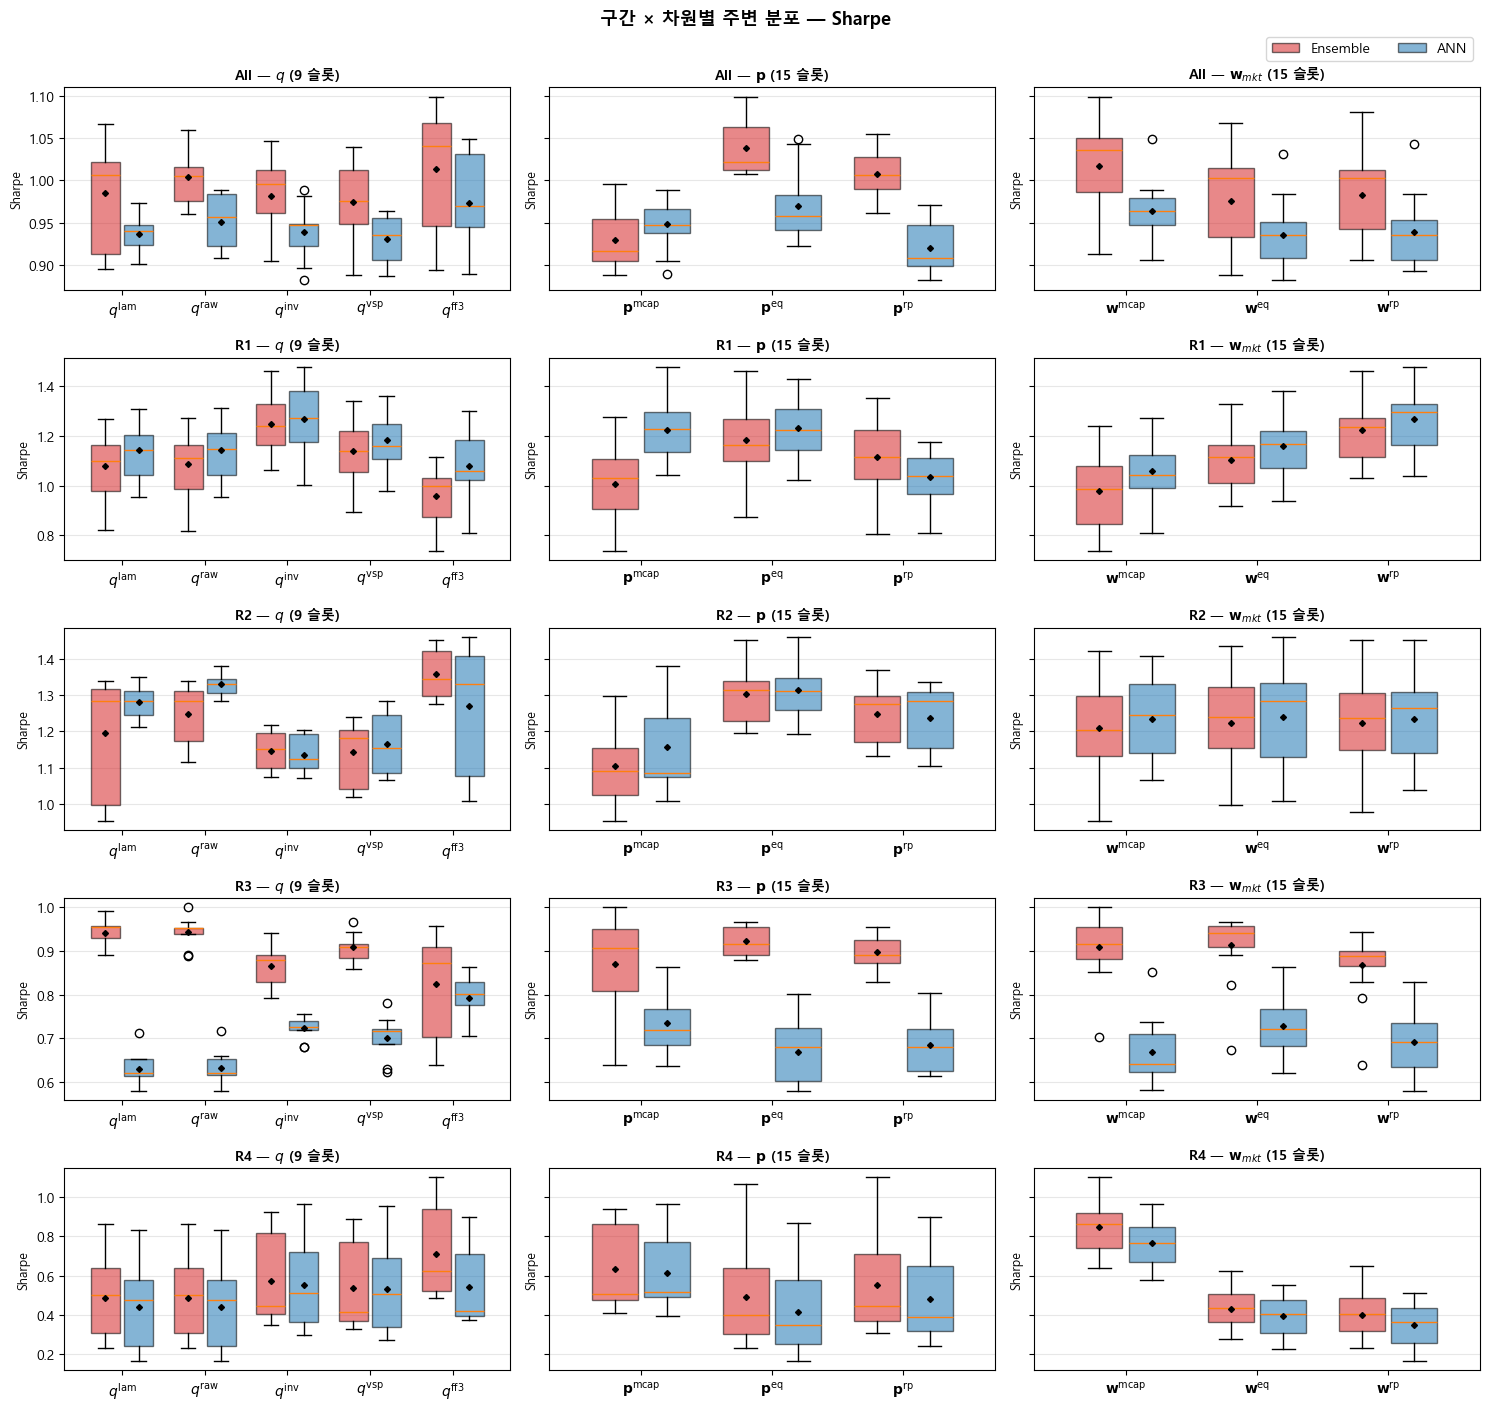
\includegraphics[width=15cm]{Figure/marginal_mean.png}
    \caption{BL 슬롯 차원별 샤프 비율 주변 분포 (앙상블 vs ANN).}
    \label{fig:marginal_boxplot}
\end{figure}

\begin{table}[t]
\centering
\caption{$\mathbf{p}$ 벡터 변경에 따른 평균 샤프 비율 ($q$ 5개 $\times$ $\mathbf{w}_{mkt}$ 3개 = 15 슬롯 평균, $\omega^{\mathrm{err}}$ 고정). 앙상블(E), ANN(A), 차이 $\Delta = \mathrm{E} - \mathrm{A}$. 녹색은 앙상블 우위, 적색은 ANN 우위.}
\label{tab:p_matrix_avg}
\setlength{\tabcolsep}{3pt}
\renewcommand{\arraystretch}{1.15}
\footnotesize
\resizebox{\textwidth}{!}{%
\begin{tabular}{l ccc ccc ccc ccc ccc}
\toprule
  & \multicolumn{3}{c}{All} & \multicolumn{3}{c}{R1} & \multicolumn{3}{c}{R2} & \multicolumn{3}{c}{R3} & \multicolumn{3}{c}{R4} \\
\cmidrule(lr){2-4} \cmidrule(lr){5-7} \cmidrule(lr){8-10} \cmidrule(lr){11-13} \cmidrule(lr){14-16}
$\mathbf{p}$ & E & A & $\Delta$ & E & A & $\Delta$ & E & A & $\Delta$ & E & A & $\Delta$ & E & A & $\Delta$ \\
\midrule
$\mathbf{p}^{\mathrm{mcap}}$ & 0.929 & 0.948 & \cellcolor{negred!50}$-0.019$ & 1.008 & 1.222 & \cellcolor{negred!50}$-0.214$ & 1.104 & 1.157 & \cellcolor{negred!50}$-0.053$ & 0.869 & 0.735 & \cellcolor{posgreen!50}$+0.134$ & 0.633 & 0.614 & \cellcolor{posgreen!50}$+0.019$ \\
$\mathbf{p}^{\mathrm{eq}}$   & 1.038 & 0.970 & \cellcolor{posgreen!50}$+0.068$ & 1.184 & 1.230 & \cellcolor{negred!50}$-0.046$ & 1.303 & 1.314 & \cellcolor{negred!50}$-0.012$ & 0.923 & 0.669 & \cellcolor{posgreen!50}$+0.253$ & 0.492 & 0.415 & \cellcolor{posgreen!50}$+0.076$ \\
$\mathbf{p}^{\mathrm{rp}}$   & 1.008 & 0.920 & \cellcolor{posgreen!50}$+0.088$ & 1.114 & 1.034 & \cellcolor{posgreen!50}$+0.081$ & 1.248 & 1.238 & \cellcolor{posgreen!50}$+0.010$ & 0.896 & 0.685 & \cellcolor{posgreen!50}$+0.212$ & 0.555 & 0.479 & \cellcolor{posgreen!50}$+0.076$ \\
\bottomrule
\end{tabular}%
}
\end{table}

R3(위기) 구간에서는 $\mathbf{p}$ 벡터 구성 방식과 무관하게 앙상블 모형이 일관된 우위를 보이며($\Delta = +0.134, +0.253, +0.212$), 표~\ref{tab:p_matrix_win}에서도 거의 모든 슬롯에서 앙상블 모형이 ANN 모형을 상회한다.
이는 변동성 분포가 가장 분산되는 위기 구간에서 앙상블 모형의 종목 순위 식별의 가치가 극대화되며, 변동성 예측 우위가 포트폴리오 성과로 가장 효과적으로 전이된다. 이러한 R3 구간에서의 우위는 Sortino 비율과 MDD에서도 유사한 패턴으로 관찰되며, 상세 슬롯별 성과 지표는 \ref{app:result_table}에 첨부하였다.

R1(회복)과 R2(확장) 구간에서는 $\mathbf{p}^{\mathrm{mcap}}$과 $\mathbf{p}^{\mathrm{eq}}$ 가중 방식 모두 앙상블 모형의 샤프 비율이 ANN 모형을 하회하는 슬롯의 빈도가 더 높지만(R1: $\mathbf{p}^{\mathrm{mcap}}$ 0/15, $\mathbf{p}^{\mathrm{eq}}$ 1/15; R2: $\mathbf{p}^{\mathrm{mcap}}, \mathbf{p}^{\mathrm{eq}}$ 모두 5/15), 손실 규모 측면에서는 두 가중치 방식 간에 명확한 차이가 존재한다. R1 구간에서 $\mathbf{p}^{\mathrm{mcap}}$의 평균 손실 $\Delta = -0.214$는 2011년 8월 미국 국가신용등급 강등 사태를 포함한 소수의 이례적 이벤트 발생 월에 손실이 집중된 결과이다. 이러한 충격은 대형주 비중 집중이 강한 $\mathbf{p}^{\mathrm{mcap}}$ 구조 하에서 증폭되어 나타났다. 반면, $\mathbf{p}^{\mathrm{eq}}$ 방식에서는 균등 배분 효과를 통해 특정 종목의 충격이 포트폴리오 전체로 전이되는 영향이 축소되어 평균 손실이 $-0.046$ 수준으로 통제된다. 즉, $\mathbf{p}^{\mathrm{eq}}$ 가중은 회복기 우위 빈도 면에서는 $\mathbf{p}^{\mathrm{mcap}}$과 유사하나, $\mathbf{p}^{\mathrm{mcap}}$의 대형주 비중 집중이 야기하는 대규모 손실 위험을 효과적으로 완화한다. 자세한 분석은 \ref{app:r1} 에서 확인할 수 있다.

그림~\ref{fig:marginal_boxplot}의 $q$ 차원을 보면, R3(위기) 구간에서 $q^{\mathrm{lam}}$과 $q^{\mathrm{raw}}$처럼 $q \geq 0$이 보장되어 저변동성 종목의 비중을 일관되게 확대하는 방식이 두 모형 간의 샤프 비율 차이를 가장 크게 만든다. 
반면 부호 제약이 없는 $q^{\mathrm{ff3}}$의 주변 분포는 R3 구간에서 $\Delta = -0.014$를 기록하여 사실상 ANN 모형과 동등 수준에 머무른다. 이 경우 다른 네 가지 $q$ 슬롯 대비 앙상블 모형의 우위는 거의 소멸한다. 단일 슬롯 기준 (\ref{subsec:baseline_slot}절, 표~\ref{tab:1step_variation})에서 관찰되었던 R3 구간의 ANN 우위($\Delta = -0.148$)가 평균값에서는 일부 희석되나, 다른 $q$ 슬롯 대비 상대적 약세는 일관되게 유지된다. 이는 앙상블 모형이 식별한 저변동성 종목의 순위 정보가 $q$의 부호가 음수로 반전되지 않는 조건에서 포트폴리오 가중치로 보다 효과적으로 보존됨을 시사한다.

본 절에서 확인한 슬롯 구성이 단순 벤치마크 대비 실제로 의미 있는 성과를 갖는지는 \ref{subsec:benchmark}절에서 확인한다.

\begin{table}[t]
\centering
\caption{$\mathbf{p}$ 벡터 변경에 따른 앙상블 우위 슬롯 수 (15 슬롯 중 $\Delta > 0$인 슬롯, $\omega^{\mathrm{err}}$ 고정).}
\label{tab:p_matrix_win}
\centering
\renewcommand{\arraystretch}{1.15}
\begin{tabular}{l ccccc}
\toprule
$\mathbf{p}$ & All & R1 & R2 & R3 & R4 \\
\midrule
$\mathbf{p}^{\mathrm{mcap}}$ & 5/15  & \cellcolor{negred!50}0/15  & 5/15 & \cellcolor{posgreen!50}12/15 & 7/15 \\
$\mathbf{p}^{\mathrm{eq}}$   & \cellcolor{posgreen!50}15/15 & \cellcolor{negred!50}1/15  & 5/15 & \cellcolor{posgreen!50}15/15 & \cellcolor{posgreen!50}15/15 \\
$\mathbf{p}^{\mathrm{rp}}$   & \cellcolor{posgreen!50}15/15 & \cellcolor{posgreen!50}14/15 & 9/15 & \cellcolor{posgreen!50}15/15 & \cellcolor{posgreen!50}15/15 \\
\bottomrule
\end{tabular}
\end{table}

\subsection{벤치마크 성능 비교}\label{subsec:benchmark}

본 절은 \ref{subsec:baseline_slot}--\ref{subsec:slot_config}절에서 확인한 변동성 예측 향상 및 슬롯 설계 효과가 표준 벤치마크 대비 실증 우위로 이어지는지 검증한다. 비교 대상은 세 외부 벤치마크(SPY, $1/N$ 동일 가중, Risk Parity) 와 \citet{pyo2018}의 ANN 앵커 슬롯(ANN-anchor: $\mathbf{w}^{\mathrm{mcap}}$, $\mathbf{p}^{\mathrm{mcap}}$, $q^{\mathrm{ff3}}$, $\omega^{\mathrm{err}}$), 변동성 예측 모형만 앙상블로 교체한 앵커 슬롯(Ensemble-anchor), 그리고 본 연구의 두 옵션(Ensemble-defensive와 Ensemble-adaptive, 각 옵션마다 $\mathbf{p}^{\mathrm{eq}}, \mathbf{p}^{\mathrm{rp}}$ 두 변형 — 총 4 슬롯)이다.

본 연구는 특정 단일 슬롯만을 최적 모형으로 권장하지 않으며, 운용 목표에 따라 선택 가능한 두 가지 옵션을 제안한다. 모든 시장 국면에서 저변동 뷰를 일관되게 유지하는 방어형 옵션(Ensemble-defensive, $q^{\mathrm{lam}}$)과, $q^{\mathrm{ff3}}$의 크기와 부호가 시장 국면에 따라 변동하는 국면 적응형 옵션(Ensemble-adaptive, $q^{\mathrm{ff3}}$)이다. 각 옵션은 $\mathbf{p}^{\mathrm{eq}}$ 또는 $\mathbf{p}^{\mathrm{rp}}$ 두 변형으로 운용할 수 있으며, 두 변형은 후술하듯 거의 동등한 성과를 보인다.

\begin{table}[t]
\centering
\caption{벤치마크 성능 비교 — 샤프 비율 $\times$ 5 기간. Ensemble 슬롯은 모두 $\mathbf{w}_{mkt} = \mathbf{w}^{\mathrm{mcap}}$ 고정, $\mathbf{p}^{\mathrm{eq}}$와 $\mathbf{p}^{\mathrm{rp}}$ 두 변형을 비교한다. MDD, Sortino 등 보조 지표는 부록~\ref{app:benchmark} 참조.}
\label{tab:benchmark_sharpe}
\setlength{\tabcolsep}{6pt}
\renewcommand{\arraystretch}{1.15}
\small
\begin{tabular}{lccccc}
\toprule
Strategy & All & R1 & R2 & R3 & R4 \\
\midrule
SPY (market)                       & 0.93 & 0.81 & 1.23 & 0.61 & 1.19 \\
$1/N$ (equal-weight)               & 0.86 & 0.78 & 1.23 & 0.70 & 0.47 \\
Risk Parity ($1/\sigma$)           & 0.89 & 0.91 & 1.28 & 0.67 & 0.45 \\
ANN-anchor \citep{pyo2018}         & 0.95 & 1.06 & 1.08 & 0.85 & 0.71 \\
Ensemble-anchor ($\sigma$ 모형 교체) & 0.95 & 0.74 & 1.29 & 0.70 & 0.94 \\
\midrule
\textbf{Ensemble-defensive} ($\mathbf{p}^{\mathrm{eq}}, q^{\mathrm{lam}}$)
                                   & 1.07 & \textbf{1.08} & 1.32 & \textbf{0.96} & 0.64 \\
\textbf{Ensemble-defensive} ($\mathbf{p}^{\mathrm{rp}}, q^{\mathrm{lam}}$)
                                   & 1.04 & 0.98 & 1.28 & 0.95 & 0.71 \\
\textbf{Ensemble-adaptive} ($\mathbf{p}^{\mathrm{eq}}, q^{\mathrm{ff3}}$)
                                   & \textbf{1.10} & 0.87 & \textbf{1.42} & 0.89 & 1.07 \\
\textbf{Ensemble-adaptive} ($\mathbf{p}^{\mathrm{rp}}, q^{\mathrm{ff3}}$)
                                   & 1.05 & 0.81 & 1.34 & 0.87 & \textbf{1.10} \\
\bottomrule
\end{tabular}
\end{table}

표~\ref{tab:benchmark_sharpe}에서 네 가지 앙상블 슬롯은 모두 외부 벤치마크와 BL 앵커 슬롯의 성과를 상회한다. 전체 분석 기간의 샤프 비율은 Ensemble-defensive가 $\mathbf{p}^{\mathrm{eq}}$ 1.07, $\mathbf{p}^{\mathrm{rp}}$ 1.04를 기록하였고, Ensemble-adaptive가 $\mathbf{p}^{\mathrm{eq}}$ 1.10, $\mathbf{p}^{\mathrm{rp}}$ 1.05를 나타냈다. 이는 $\mathbf{p}$ 벡터 변형 선택과 무관하게 전통적 벤치마크인 SPY(0.93), $1/N$ 동일 가중(0.86), Risk Parity(0.89) 및 ANN-anchor(0.95) 성과를 모두 능가하는 수치이다. MDD 측면에서도 네 가지 Ensemble 슬롯은 SPY 및 ANN-anchor 대비 더 얕은 손실을 기록하며, 특히 Ensemble-defensive 두 변형의 방어력이 가장 우수하다. 이와 관련한 상세 수치는~\ref{app:benchmark}에 수록하였다.

Ensemble-anchor의 전체 분석 기간 샤프 비율은 0.95를 기록하여 ANN-anchor와 사실상 동률이다. 즉 기존 앵커 슬롯 구조를 유지한 채 변동성 예측 모형만 앙상블로 교체하는 방식으로는 실제 포트폴리오의 성과 개선이 거의 발생하지 않는다. 반면 $\mathbf{p}$ 벡터 가중치 방식을 $\mathbf{p}^{\mathrm{mcap}}$에서 $\mathbf{p}^{\mathrm{eq}}$ 또는 $\mathbf{p}^{\mathrm{rp}}$로 변경할 경우, 두 앙상블 옵션 모두 $+0.09 \sim +0.15$의 샤프 비율 개선이 일관되게 나타난다. 이는 변동성 예측력 우위(표~\ref{tab:sigma_pred})가 포트폴리오 성과로 전이되는 결정적 통로가 슬롯 설계, 특히 $\mathbf{p}$ 가중치의 대형주 비중 집중 완화에 있음을 보여주며, $\mathbf{p}^{\mathrm{eq}}$와 $\mathbf{p}^{\mathrm{rp}}$가 거의 동등한 개선 효과를 제공한다.

또한, 두 가지 앙상블 옵션은 시장 국면에 따라 보완적인 강점을 보인다. Ensemble-defensive는 R1(회복) 국면과 R3(위기) 국면 등 시장 변동성이 상승하는 구간에서 강점을 보인다($\mathbf{p}^{\mathrm{eq}}$ 기준 샤프 비율 각각 1.08, 0.96). 이는 $q^{\mathrm{lam}}$의 양수 제약이 모든 시점에서 저변동 뷰를 일관되게 유지하기 때문이다. 반면 Ensemble-adaptive는 R2(확장) 국면과 R4(정상화) 강세장 국면에서 강점을 보인다($\mathbf{p}^{\mathrm{eq}}$ 기준 샤프 비율 각각 1.42, 1.07). 이는 $q^{\mathrm{ff3}}$의 FF3 회귀 기반 구조가 강세장에서 뷰를 적응적으로 재조정함으로써 상승장 포착 능력을 제공하기 때문이다. R3(위기) 국면에서는 두 옵션의 네 가지 변형 슬롯이 모두 ANN-anchor(0.85)를 상회하였으며($0.87 \sim 0.96$), R4 강세장 국면에서는 Ensemble-adaptive의 두 변형 슬롯이 ANN-anchor(0.71)를 크게 상회하는 성과(1.07, 1.10)를 기록했다. 한편 $\mathbf{p}$ 가중 방식의 효과는 시장 국면에 따라 비대칭적으로 작동하는 특성을 보였다. R1 국면에서는  $\mathbf{p}^{\mathrm{eq}}$ 방식이 $\mathbf{p}^{\mathrm{rp}}$ 방식 대비 Ensemble-defensive에서 약 0.10, Ensemble-adaptive에서 약 0.06의 성과 우위를 나타냈다. 반대로 R4 국면에서는 $\mathbf{p}^{\mathrm{rp}}$ 방식이 두 옵션 모두에서 $\mathbf{p}^{\mathrm{eq}}$ 방식을 약간 상회하는 결과(Ensemble-defensive 0.71 vs 0.64, Ensemble-adaptive 1.10 vs 1.07)를 보였다.

\begin{figure}[t]
\centering
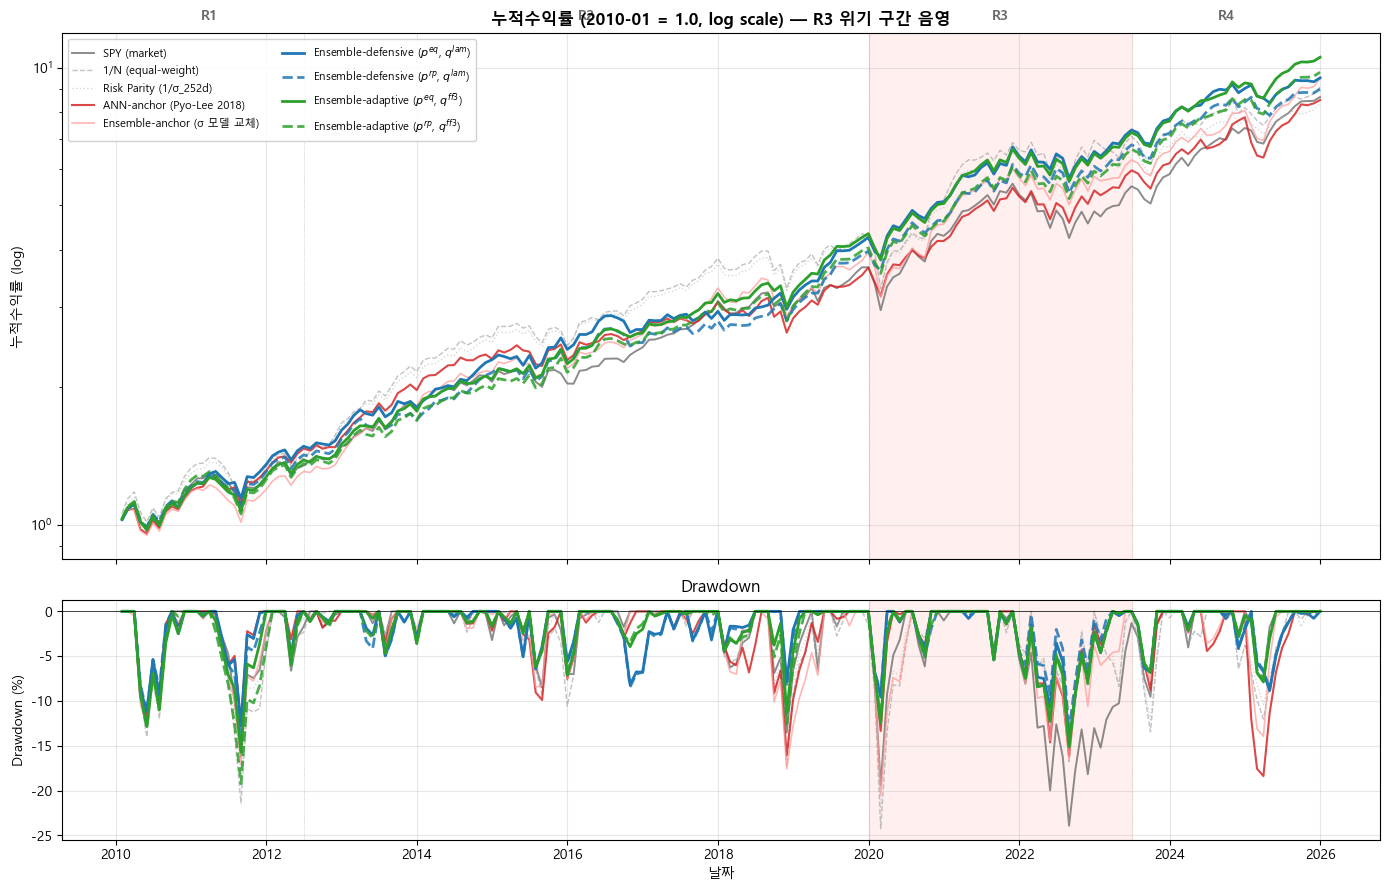
\includegraphics[width=\textwidth]{Figure/benchmark_plot.png}
\caption{누적수익률(상단, log scale) 및 drawdown(하단), 2010-01\textendash 2025-12. R3(위기) 국면 음영. 파랑=Ensemble-defensive, 초록=Ensemble-adaptive.}
\label{fig:benchmark_cumret}
\end{figure}

Ensemble-defensive와 Ensemble-adaptive는 전체 분석 기간 샤프 비율과 누적 수익률이 거의 동등하지만(그림~\ref{fig:benchmark_cumret}), 국면별 성과 구성이 상이하므로 운용 목표에 따라 선택할 수 있다. 저변동 정체성을 모든 시장 국면에서 엄격히 유지하려는 보수적 운용 방식에는 Ensemble-defensive가, 강세장에서의 추가 상승 수익을 일정 부분 허용하는 적응적 운용 방식에는 Ensemble-adaptive가 적합하다. 두 가지 옵션 모두 표준 벤치마크 대비 유의미한 성과 우위를 제공하며, $\mathbf{p}^{\mathrm{eq}}$와 $\mathbf{p}^{\mathrm{rp}}$ 어느 가중 방식을 적용하더라도 일관된 성과를 보여 $\mathbf{p}$ 변형 선택에 강건하다. $q^{\mathrm{ff3}}$이 강세장에서 뷰를 적응적으로 재조정하는 구체적 메커니즘 및 $\mathbf{p}$ 가중치의 완화 효과는 \ref{app:r4_mechanism}에서 상세히 분석한다.







\section{결론 및 한계}\label{sec:conclusion}

본 연구는 \citet{pyo2018}의 KOSPI 200 BL 저변동 프레임워크를 S\&P 500 시장에 적용하면서, 변동성 예측 모형과 BL 슬롯 구성을 재검토하고 2010--2025년 192개월을 4개 시장 국면(R1 회복, R2 확장, R3 위기, R4 정상화)으로 분해하여 평가하였다. 단일 슬롯 비교에 그치지 않고 90개 슬롯을 차원별($\mathbf{p} \times \mathbf{w}_{mkt} \times q \times \omega$)로 분해하여 주변 분포를 산출하고, 이를 4개 국면으로 재분해하는 프레임워크를 통해 운용 목표에 따른 슬롯 선택 근거를 제시한 점이 본 연구의 분석적 기여이다.

LSTM-HAR 앙상블 모형은 ANN 모형 대비 변동성 예측 정확도(RMSE, Spearman, Hit Rate)에서 전 구간 일관된 우위를 보였으며, 특히 R3(위기) 국면에서 격차가 전체 분석 기간 대비 약 1.5-2배 확대되었다(RMSE 격차는 전구간과 유사한 수준 유지). R3 국면은 COVID-19 팬데믹 충격(2020년 1\textendash 2분기)과 2022년 긴축 약세장이 복합된 시기로, 시장 전반의 변동성 수준과 종목 간 변동성 격차가 모두 극대화된 환경이었다. 이러한 국면에서는 종목별 변동성 순위가 빠르게 재편되며, 이를 안정적으로 식별하는 능력이 포트폴리오 성과에 가장 결정적으로 작용한 것으로 해석된다. 다만 이러한 예측 우위가 포트폴리오 성과로 전이되기 위해서는 슬롯 설계, 특히 $\mathbf{p}$ 벡터의 대형주 비중 집중 완화가 동반되어야 한다. 변동성 예측 모형만 앙상블로 교체한 Ensemble-anchor는 ANN-anchor와 샤프 비율이 동률(0.95)에 머무르나, $\mathbf{p}$ 가중치를 $\mathbf{p}^{\mathrm{eq}}$ 또는 $\mathbf{p}^{\mathrm{rp}}$로 변경하면 두 슬롯 구성 모두 $+0.09 \sim +0.15$의 샤프 비율 개선이 일관되게 나타난다.
본 연구는 자산배분 프로세스에서 단일한 최적 슬롯 설정을 고집하기보다, 운용 목표에 따라 BL의 입력 변수를 유연하게 다원화할 수 있는 실무적 가이드라인을 제시하였다. 모든 시장 국면에서 저변동 정체성을 엄격히 유지하려는 보수적 운용에는 $q^{lam}$‬기반의 Ensemble-defensive가, 강세장 국면에서 시장 랠리를 추종하여 초과 수익을 추구하는 동적 자산 배분에는 $q^{ff3}$‬ 기반의 Ensemble-adaptive가 유용한 대안이 될 수 있음을 확인하였다. 두 전략 모두 $\mathbf{p}^{\mathrm{eq}}$와 $\mathbf{p}^{\mathrm{rp}}$‬ 중 어느 변형을 선택하더라도, 편측 20bp의 거래비용을 차감 후 전통적 벤치마크 및 ANN-anchor를 전 구간에 걸쳐 일관되게 상회하였다. 이는 변동성 예측 모형의 고도화가 단일한 최적 슬롯 구조에 국한되지 않고, 운용 목표에 맞는 유연한 BL 입력 설계와 결합될 때 실질적인 위험조정수익률 제고로 이어질 수 있음을 시사한다.

본 연구는 다음과 같은 한계를 가진다. 첫째, 야후 파이낸스 데이터의 가용성 제약으로 인해 833개 종목 중 216개가 분석에서 누락되어 최종 617개 종목만을 대상으로 실증 분석을 수행하였다. 시점별 멤버십 필터링을 통해 생존 편향을 완화하였으나, 이러한 가용성 한계는 포트폴리오의 절대 성과를 과대 추정하는 방향과 위기 구간에 사라진 고변동 종목의 누락으로 인해 저변동성 우위 자체를 과소 추정하는 방향으로 동시에 작용할 수 있어, 편향의 방향을 단정하기 어렵다.

둘째, 본 연구가 사용한 LSTM 모형은 4채널($\mathrm{RV}_{d/w/m}$, $\log(\mathrm{VIX})$)의 입력 피처와 단일 은닉층으로 구성된 단순한 구조다. 따라서 향후 거시 경제 변수, 뉴스 감성 정보, 옵션 시장 정보 등을 추가 자산 신호로 반영하고, 모형을 다층(Multi-layer) 및 어텐션(Attention) 구조로 고도화할 경우 예측 정확도를 추가적으로 개선할 여지가 있다.

셋째, 본 연구에서 관찰된 국면별 성과 결과와 슬롯 메커니즘은 실증적 관찰에 머무르며 인과적 규명에 이르지 못한다. R1(회복) 국면에서 관측된 앙상블 모형 약세의 시점 집중성(\ref{app:r1}절)과 강세장 국면에서 발생한 $q^{\mathrm{ff3}}$의 부호 반전 현상(\ref{app:r4_mechanism}절) 역시 직관적인 합리성을 넘어선 인과적 검증은 본 연구의 분석 범위를 벗어난다. 향후 연구에서는 예측 모형 고도화, 데이터 가용성의 추가 확보, 그리고 슬롯 간 인과적 분해를 통해 본 연구의 실증적 발견을 보완할 필요가 있다.


% --------------- appendix 시작 ---------------
% KJAS 양식에서는 부록 수식·표·그림이 자동으로 A.1, A.2 ... 형식으로 부여됨.
\appendix

\section{HMM 기반 시장 국면 분류}\label{app:hmm}

Hidden Markov Model(HMM, \citealp{hamilton1989new})은 관측 불가능한 잠재 상태인 시장 국면(Regime)이 확률적으로 전이하며 관측 데이터를 생성한다고 가정하는 통계 모형으로, 시장 국면처럼 직접 관측되지 않는 구조적 상태를 데이터를 기반으로 식별하는 데 적합하다. 본 연구는 HMM을 활용하여 분석 기간(2010-2025)의 시장 국면을 사후적으로 정의하고, 이를 포트폴리오 성과 분해의 기준으로 활용한다.

\subsection*{A1 데이터 및 학습 기간}

HMM 학습에는 Fama-French 5팩터(Fama-French 5-factor model, FF5)(일별), 매크로 지표 5개(VIX, 장단기 금리차 등), 그리고 개별 종목 일별 수익률로부터 산출한 동일 가중 시장 수익률을 결합한 데이터를 사용하였다. 학습 기간은 2004년 4월부터 2026년 2월까지이며, 유효 거래일은 총 5,512일이다.

HMM은 실시간 트레이딩 신호 생성이 아닌 사후적 시장 국면 정의가 목적이므로, 전체 구간 학습 방식의 미래 정보 반영 문제(look-ahead bias)는 본 연구의 분석 목적상 해당되지 않는다. 또한 국면 레이블은 BL 모형 학습 과정에 직접 투입되지 않으므로 정보 누설 경로도 없다.

\subsection*{A2 입력 피처}

16개 후보 피처 중 이론적 근거를 먼저 적용하고, ADF 단위근 검정·상관 행렬·분산팽창지수(VIF) 다중공선성 검증을 통해 최종 6개 피처를 선별하였다(표~\ref{tab:a1_features}). 통계 검증은 전체 데이터를 기반으로 계산하였으며, 입력 데이터는 Z-score 방식으로 표준화 후 HMM에 투입하였다.

\begin{table}[t]
\centering
\caption{HMM 입력 피처 선택 결과}
\label{tab:a1_features}
\begin{tabular}{lll}
\toprule
\textbf{피처} & \textbf{설명} & \textbf{선택 근거} \\
\midrule
\texttt{mkt\_rf}       & 시장 초과수익률 (일별)     & Bull/Bear 구분의 직접 수익 신호 \\
\texttt{vol\_21d\_daily} & 21일 실현변동성           & 국면 라벨링 기준 (변동성 순 정렬) \\
\texttt{vol\_ratio}    & 단기/장기 변동성 비율      & 국면 전환 선행 신호 ($>$1이면 변동성 급증) \\
\texttt{vix\_basis}    & 기대변동성 $-$ 실현변동성  & 패닉 국면 식별 (음수 $=$ 공포 실현, Bear/Crisis) \\
\texttt{t10y2y\_chg}   & 장단기 금리차 1차 차분     & 경기 국면 변화 선행지표 (ADF 비정상으로 대체) \\
\texttt{mom}           & 모멘텀 팩터               & 추세 지속성 (Bull: 양수, Bear: 음수) \\
\bottomrule
\end{tabular}
\end{table}

\subsection*{A3 모형 설정 및 국면 수 선택}

Gaussian HMM을 사용하였으며, 방출 분포는 국면별 독립적인 완전 공분산 행렬(full covariance) 구조로 설정하였다. $n = 3, 4, 5$에 대해 전체 기간 HMM을 각각 학습하고 국면 안정성과 경제적 해석 가능성을 기준으로 최적 국면 수를 비교하였다.

$n = 4$ 및 $n = 5$에서 추가로 분리되는 국면은 Bull이 Mild\_Bull로 세분화되는 형태이나, 이 세분화가 GFC(글로벌 금융위기)·COVID·2022 Bear 등 기존 시장 사건과의 대응 관계에서 $n = 3$ 대비 명확한 우위를 보이지 않는다. Bear 및 위기 구간은 $n$에 관계없이 일관되게 포착되므로, 경제적 해석 가능성과 국면 레이블 단순성을 기준으로 $n = 3$을 최종 채택하였다. 국면 레이블은 각 국면의 평균 \texttt{vol\_21d\_daily} 값 기준 오름차순으로 Bull(저변동·강세), Neutral(중변동·중립), Bear(고변동·약세) 순서로 부여하였다.

$n = 3, 4, 5$ 비교 결과, $n$이 커질수록 평균 최대 사후 확률이 낮아지며($n=3$: 0.984, $n=4$: 0.971, $n=5$: 0.976), 고확신 구간($\geq 90\%$) 비율도 감소한다. $n = 3$에서 전체 거래일의 94.5\%가 고확신 구간에 해당해 국면 레이블 신뢰성이 가장 우수하였으며, 이를 최종 채택하였다.

\begin{table}[t]
\centering
\caption{국면 분류 모형 확신도}
\label{tab:a1_confidence}
\begin{tabular}{ccccc}
\toprule
\textbf{$n$} & \textbf{평균 최대 사후 확률} & \textbf{$\geq$90\% 고확신} & \textbf{70$\sim$90\%} & \textbf{$<$70\% 불확실} \\
\midrule
3 & 0.984 & 94.5\% (5,207일) & 3.8\% (207일) & 1.8\% (98일) \\
4 & 0.971 & 90.9\% (5,012일) & 5.5\% (301일) & 3.6\% (199일) \\
5 & 0.976 & 92.2\% (5,084일) & 5.1\% (279일) & 2.7\% (149일) \\
\bottomrule
\end{tabular}
\begin{flushleft}
{\small $^*$ 최대 사후 확률: 각 거래일에서 가장 높은 국면 소속 사후 확률.}
\end{flushleft}
\end{table}

\subsection*{A4 국면별 기초 통계}

$n = 3$ 기준 각 국면의 기초 통계는 표~\ref{tab:a1_stats}와 같다. Bear 국면의 일평균 변동성은 Bull 대비 약 3.5배(2.271\% / 0.653\%), VIX는 약 2.5배(35.0 / 14.0)로 높다. 일평균 수익률·변동성·VIX 모두 Bull $\rightarrow$ Neutral $\rightarrow$ Bear 순서로 단조 증가/감소하여, 각 국면이 서로 다른 시장 체질을 나타냄을 확인하였다.

\begin{table}[t]
\centering
\caption{국면별 기초 통계 ($n=3$)}
\label{tab:a1_stats}
\begin{tabular}{lccccc}
\toprule
\textbf{국면} & \textbf{비중} & \textbf{거래일} & \textbf{일평균 수익률} & \textbf{일평균 변동성} & \textbf{평균 VIX} \\
\midrule
Bull    & 52.9\% & 2,914일 & $+$0.063\% & 0.653\% & 14.0 \\
Neutral & 34.1\% & 1,877일 & $+$0.025\% & 1.070\% & 20.7 \\
Bear    & 13.1\% &   721일 & $-$0.002\% & 2.271\% & 35.0 \\
\bottomrule
\end{tabular}
\begin{flushleft}
{\small $^*$ 수익률 및 변동성은 일별 단위. VIX는 연환산 \% (참고 수치).}
\end{flushleft}
\end{table}

\subsection*{A5 전이 행렬}

$n = 3$ 기준 일별 국면 전이 행렬은 표~\ref{tab:a1_trans}와 같다. 대각선(자기전이) 확률이 0.969 이상으로, 국면은 일별 노이즈가 아닌 수 주$\sim$수 달 단위로 지속되는 안정적 상태임을 확인하였다. Bull $\leftrightarrow$ Bear 직접 전이 확률은 사실상 0으로, 국면 전환은 인접 상태를 경유해 점진적으로 이루어진다. 이러한 높은 국면 지속성은 국면 신호를 월별 리밸런싱 전략에 활용하기 위한 충분한 조건이 된다.

\begin{table}[t]
\centering
\caption{전이 행렬 ($n=3$, 일별)}
\label{tab:a1_trans}
\begin{tabular}{lccc}
\toprule
 & \textbf{$\rightarrow$ Bull} & \textbf{$\rightarrow$ Neutral} & \textbf{$\rightarrow$ Bear} \\
\midrule
\textbf{Bull}    & 0.987 & 0.012 & $\sim$0 \\
\textbf{Neutral} & 0.019 & 0.970 & 0.011 \\
\textbf{Bear}    & $\sim$0 & 0.031 & 0.969 \\
\bottomrule
\end{tabular}
\end{table}

\subsection*{A6 구조적 전환점}

비터비(Viterbi) 알고리즘으로 추출한 최적 국면 경로에서 이전 국면 $\geq$ 63거래일(약 3개월), 새 국면 $\geq$ 63거래일을 동시에 충족하는 경우만 구조적 전환점으로 정의하여 단기 노이즈를 제거하였다. 추출된 전환점은 표~\ref{tab:a1_breaks}와 같으며, post-GFC 본격 강세(2012), COVID 직전 강세(2019), AI 랠리 시작(2023) 등 실제 시장 사건과 시기적으로 일치한다.

\begin{table}[t]
\centering
\caption{구조적 전환점 ($n=3$ 기준, 양방향 $\geq$ 63거래일 조건)}
\label{tab:a1_breaks}
\begin{tabular}{llll}
\toprule
\textbf{전환일} & \textbf{전환 방향} & \textbf{대응 시장 사건} & \textbf{비고} \\
\midrule
2012-08-15 & Neutral $\rightarrow$ Bull & post-GFC 본격 강세      & R1/R2 경계 근거 \\
2019-11-05 & Neutral $\rightarrow$ Bull & COVID 직전 강세         & R2/R3 경계 근거 \\
2023-06-05 & Bear/Neutral $\rightarrow$ Bull & AI 랠리 시작       & R3/R4 경계 근거 \\
2024-08-01 & Bull $\rightarrow$ Neutral & 2024 금리 인하 기대 후퇴 & 분석 기간 내 마지막 전환점 \\
\bottomrule
\end{tabular}
\end{table}

$n = 3$ 기준 전환점(2023-06-05)을 분기말로 조정하여 R3와 R4의 경계를 2023년 6월 말로 설정하였다. 2024-08-01 전환점(Bull $\rightarrow$ Neutral)은 R4 내부의 국면 변화로, 평가 국면 경계 조정에는 반영하지 않았다.

\subsection*{A7 평가 국면 정의}

HMM 전환점을 분기말 기준으로 조정하고, COVID 시작 및 AI 랠리를 경제적 직관에 맞추어, 본 연구의 평가 구간을 표~\ref{tab:a1_regimes}와 같이 4개 국면으로 정의하였다.

\begin{table}[t]
\centering
\caption{본 연구 평가 국면 정의}
\label{tab:a1_regimes}
\begin{tabular}{llcl}
\toprule
\textbf{국면} & \textbf{기간} & \textbf{거래일} & \textbf{해석} \\
\midrule
R1 & 2010-01 $\sim$ 2012-06 (30개월) & 약 630일   & GFC 회복·유럽 재정위기 구간 \\
R2 & 2012-07 $\sim$ 2019-12 (90개월) & 약 1,890일 & 저변동 장기 확장 구간 \\
R3 & 2020-01 $\sim$ 2023-06 (42개월) & 약 882일   & COVID 충격·2022 긴축으로 인한 고변동성 복합 국면 구간 \\
R4 & 2023-07 $\sim$ 2025-12 (30개월) & 약 630일   & AI 주도 랠리 (정상화) \\
\bottomrule
\end{tabular}
\end{table}

\section{슬롯 분석 결과 전체 표}\label{app:result_table}

\ref{subsec:slot_config}절의 평균 결과(표~\ref{tab:p_matrix_avg})를 보완하여, 90 슬롯 전체의 성과를 뷰 신뢰도 $\omega \in \{\omega^{\mathrm{err}}, \omega^{\mathrm{he}}\}$와 평가 지표 $\in \{\text{Sharpe}, \text{Sortino}, \text{MDD}\}$의 6개 조합 표로 제공한다. 표~\ref{tab:app_grid_sharpe_err}--\ref{tab:app_grid_mdd_err}는 $\omega = \omega^{\mathrm{err}}$ 기준, 표~\ref{tab:app_grid_sharpe_he}--\ref{tab:app_grid_mdd_he}는 $\omega = \omega^{\mathrm{he}}$ 기준이다.

평가 지표는 다음 세 가지를 사용한다.
\begin{itemize}
  \item \textbf{Sharpe 비율}: 평균 초과수익을 표준편차로 나눈 위험 조정 수익률. 클수록 우위.
  \item \textbf{Sortino 비율}: 샤프 비율의 하방 변동성 버전으로, 분모를 하방 표준편차로 대체한다\citep{sortino1994}. 하락 변동성만 페널티로 반영하며 클수록 우위.
  \item \textbf{최대낙폭 (MDD)}: 누적 고점 대비 최대 손실 폭(\%). 음수가 손실이므로 클수록(0 에 가까울수록) 우위.
\end{itemize}
따라서 모든 표의 $\Delta > 0$ 셀(녹색)은 앙상블이 ANN 대비 위험 조정 수익 또는 손실 폭 측면에서 우위인 경우이다.

\begin{table}[t]
\centering
\caption{전체 45 슬롯 Sharpe 비율 결과 ($\omega = \omega^{\mathrm{err}}$ 고정).
$\mathbf{p} \times \mathbf{w}_{mkt} \times q = 3 \times 3 \times 5 = 45$ 슬롯 각각의
앙상블(E) · ANN(A) Sharpe 비율 및 차이 $\Delta = \mathrm{E} - \mathrm{A}$를
5개 구간 (All, R1 회복, R2 확장, R3 위기, R4 정상화)에 대해 보고한다.}
\label{tab:app_grid_sharpe_err}
\setlength{\tabcolsep}{2pt}
\renewcommand{\arraystretch}{1.05}
\scriptsize
\resizebox{\textwidth}{!}{%
\begin{tabular}{lll ccc ccc ccc ccc ccc}
\toprule
 & & & \multicolumn{3}{c}{All} & \multicolumn{3}{c}{R1} & \multicolumn{3}{c}{R2} & \multicolumn{3}{c}{R3} & \multicolumn{3}{c}{R4} \\
\cmidrule(lr){4-6} \cmidrule(lr){7-9} \cmidrule(lr){10-12} \cmidrule(lr){13-15} \cmidrule(lr){16-18}
$\mathbf{p}$ & $\mathbf{w}_{mkt}$ & $q$ & E & A & $\Delta$ & E & A & $\Delta$ & E & A & $\Delta$ & E & A & $\Delta$ & E & A & $\Delta$ \\
\midrule
$\mathbf{p}^{\mathrm{mcap}}$ & $\mathbf{w}^{\mathrm{mcap}}$ & $q^{\mathrm{lam}}$ & $0.913$ & $0.952$ & \cellcolor{negred!50}$-0.038$ & $0.821$ & $1.041$ & \cellcolor{negred!50}$-0.220$ & $0.953$ & $1.213$ & \cellcolor{negred!50}$-0.260$ & $0.991$ & $0.638$ & \cellcolor{posgreen!50}$+0.353$ & $0.864$ & $0.833$ & \cellcolor{posgreen!50}$+0.030$ \\
 &  & $q^{\mathrm{raw}}$ & $0.976$ & $0.988$ & \cellcolor{negred!50}$-0.012$ & $0.818$ & $1.044$ & \cellcolor{negred!50}$-0.226$ & $1.115$ & $1.332$ & \cellcolor{negred!50}$-0.217$ & $0.999$ & $0.643$ & \cellcolor{posgreen!50}$+0.357$ & $0.864$ & $0.833$ & \cellcolor{posgreen!50}$+0.030$ \\
 &  & $q^{\mathrm{inv}}$ & $0.995$ & $0.982$ & \cellcolor{posgreen!50}$+0.014$ & $1.061$ & $1.244$ & \cellcolor{negred!50}$-0.183$ & $1.100$ & $1.084$ & \cellcolor{posgreen!50}$+0.016$ & $0.894$ & $0.738$ & \cellcolor{posgreen!50}$+0.156$ & $0.915$ & $0.963$ & \cellcolor{negred!50}$-0.048$ \\
 &  & $q^{\mathrm{vsp}}$ & $0.949$ & $0.948$ & $+0.000$ & $0.894$ & $1.105$ & \cellcolor{negred!50}$-0.211$ & $1.030$ & $1.067$ & \cellcolor{negred!50}$-0.037$ & $0.943$ & $0.720$ & \cellcolor{posgreen!50}$+0.223$ & $0.891$ & $0.958$ & \cellcolor{negred!50}$-0.067$ \\
 &  & $q^{\mathrm{ff3}}$ & $0.946$ & $0.945$ & $+0.000$ & $0.738$ & $1.059$ & \cellcolor{negred!50}$-0.321$ & $1.287$ & $1.076$ & \cellcolor{posgreen!50}$+0.212$ & $0.702$ & $0.850$ & \cellcolor{negred!50}$-0.148$ & $0.940$ & $0.712$ & \cellcolor{posgreen!50}$+0.228$ \\
\cmidrule(lr){2-18}
 & $\mathbf{w}^{\mathrm{eq}}$ & $q^{\mathrm{lam}}$ & $0.895$ & $0.947$ & \cellcolor{negred!50}$-0.052$ & $0.979$ & $1.168$ & \cellcolor{negred!50}$-0.189$ & $0.997$ & $1.245$ & \cellcolor{negred!50}$-0.248$ & $0.956$ & $0.711$ & \cellcolor{posgreen!50}$+0.244$ & $0.505$ & $0.518$ & \cellcolor{negred!50}$-0.014$ \\
 &  & $q^{\mathrm{raw}}$ & $0.961$ & $0.984$ & \cellcolor{negred!50}$-0.023$ & $0.988$ & $1.163$ & \cellcolor{negred!50}$-0.176$ & $1.175$ & $1.382$ & \cellcolor{negred!50}$-0.207$ & $0.965$ & $0.717$ & \cellcolor{posgreen!50}$+0.248$ & $0.505$ & $0.518$ & \cellcolor{negred!50}$-0.014$ \\
 &  & $q^{\mathrm{inv}}$ & $0.905$ & $0.940$ & \cellcolor{negred!50}$-0.035$ & $1.164$ & $1.381$ & \cellcolor{negred!50}$-0.217$ & $1.075$ & $1.072$ & \cellcolor{posgreen!50}$+0.003$ & $0.823$ & $0.756$ & \cellcolor{posgreen!50}$+0.066$ & $0.455$ & $0.551$ & \cellcolor{negred!50}$-0.096$ \\
 &  & $q^{\mathrm{vsp}}$ & $0.888$ & $0.927$ & \cellcolor{negred!50}$-0.038$ & $1.042$ & $1.226$ & \cellcolor{negred!50}$-0.184$ & $1.018$ & $1.077$ & \cellcolor{negred!50}$-0.059$ & $0.905$ & $0.780$ & \cellcolor{posgreen!50}$+0.125$ & $0.437$ & $0.538$ & \cellcolor{negred!50}$-0.101$ \\
 &  & $q^{\mathrm{ff3}}$ & $0.894$ & $0.889$ & \cellcolor{posgreen!50}$+0.006$ & $0.919$ & $1.182$ & \cellcolor{negred!50}$-0.262$ & $1.276$ & $1.007$ & \cellcolor{posgreen!50}$+0.269$ & $0.673$ & $0.862$ & \cellcolor{negred!50}$-0.189$ & $0.623$ & $0.420$ & \cellcolor{posgreen!50}$+0.202$ \\
\cmidrule(lr){2-18}
 & $\mathbf{w}^{\mathrm{rp}}$ & $q^{\mathrm{lam}}$ & $0.905$ & $0.946$ & \cellcolor{negred!50}$-0.041$ & $1.106$ & $1.295$ & \cellcolor{negred!50}$-0.189$ & $0.977$ & $1.229$ & \cellcolor{negred!50}$-0.252$ & $0.928$ & $0.653$ & \cellcolor{posgreen!50}$+0.276$ & $0.502$ & $0.478$ & \cellcolor{posgreen!50}$+0.024$ \\
 &  & $q^{\mathrm{raw}}$ & $0.966$ & $0.983$ & \cellcolor{negred!50}$-0.017$ & $1.110$ & $1.296$ & \cellcolor{negred!50}$-0.185$ & $1.133$ & $1.353$ & \cellcolor{negred!50}$-0.220$ & $0.942$ & $0.659$ & \cellcolor{posgreen!50}$+0.283$ & $0.502$ & $0.478$ & \cellcolor{posgreen!50}$+0.024$ \\
 &  & $q^{\mathrm{inv}}$ & $0.916$ & $0.947$ & \cellcolor{negred!50}$-0.031$ & $1.274$ & $1.478$ & \cellcolor{negred!50}$-0.204$ & $1.090$ & $1.098$ & \cellcolor{negred!50}$-0.008$ & $0.793$ & $0.720$ & \cellcolor{posgreen!50}$+0.073$ & $0.431$ & $0.512$ & \cellcolor{negred!50}$-0.081$ \\
 &  & $q^{\mathrm{vsp}}$ & $0.909$ & $0.935$ & \cellcolor{negred!50}$-0.027$ & $1.167$ & $1.346$ & \cellcolor{negred!50}$-0.179$ & $1.039$ & $1.086$ & \cellcolor{negred!50}$-0.046$ & $0.881$ & $0.742$ & \cellcolor{posgreen!50}$+0.138$ & $0.409$ & $0.506$ & \cellcolor{negred!50}$-0.097$ \\
 &  & $q^{\mathrm{ff3}}$ & $0.918$ & $0.904$ & \cellcolor{posgreen!50}$+0.014$ & $1.032$ & $1.299$ & \cellcolor{negred!50}$-0.267$ & $1.298$ & $1.038$ & \cellcolor{posgreen!50}$+0.260$ & $0.638$ & $0.829$ & \cellcolor{negred!50}$-0.191$ & $0.651$ & $0.394$ & \cellcolor{posgreen!50}$+0.257$ \\
\midrule
$\mathbf{p}^{\mathrm{eq}}$ & $\mathbf{w}^{\mathrm{mcap}}$ & $q^{\mathrm{lam}}$ & $1.067$ & $0.973$ & \cellcolor{posgreen!50}$+0.094$ & $1.076$ & $1.120$ & \cellcolor{negred!50}$-0.045$ & $1.320$ & $1.335$ & \cellcolor{negred!50}$-0.016$ & $0.956$ & $0.583$ & \cellcolor{posgreen!50}$+0.373$ & $0.638$ & $0.578$ & \cellcolor{posgreen!50}$+0.059$ \\
 &  & $q^{\mathrm{raw}}$ & $1.060$ & $0.976$ & \cellcolor{posgreen!50}$+0.084$ & $1.085$ & $1.125$ & \cellcolor{negred!50}$-0.040$ & $1.311$ & $1.345$ & \cellcolor{negred!50}$-0.034$ & $0.953$ & $0.583$ & \cellcolor{posgreen!50}$+0.370$ & $0.638$ & $0.578$ & \cellcolor{posgreen!50}$+0.059$ \\
 &  & $q^{\mathrm{inv}}$ & $1.047$ & $0.988$ & \cellcolor{posgreen!50}$+0.059$ & $1.240$ & $1.270$ & \cellcolor{negred!50}$-0.030$ & $1.195$ & $1.205$ & \cellcolor{negred!50}$-0.010$ & $0.878$ & $0.681$ & \cellcolor{posgreen!50}$+0.197$ & $0.816$ & $0.720$ & \cellcolor{posgreen!50}$+0.097$ \\
 &  & $q^{\mathrm{vsp}}$ & $1.040$ & $0.963$ & \cellcolor{posgreen!50}$+0.076$ & $1.131$ & $1.158$ & \cellcolor{negred!50}$-0.028$ & $1.205$ & $1.245$ & \cellcolor{negred!50}$-0.040$ & $0.914$ & $0.624$ & \cellcolor{posgreen!50}$+0.291$ & $0.772$ & $0.688$ & \cellcolor{posgreen!50}$+0.084$ \\
 &  & $q^{\mathrm{ff3}}$ & $1.099$ & $1.049$ & \cellcolor{posgreen!50}$+0.050$ & $0.872$ & $1.024$ & \cellcolor{negred!50}$-0.152$ & $1.421$ & $1.408$ & \cellcolor{posgreen!50}$+0.013$ & $0.888$ & $0.705$ & \cellcolor{posgreen!50}$+0.183$ & $1.066$ & $0.868$ & \cellcolor{posgreen!50}$+0.198$ \\
\cmidrule(lr){2-18}
 & $\mathbf{w}^{\mathrm{eq}}$ & $q^{\mathrm{lam}}$ & $1.022$ & $0.935$ & \cellcolor{posgreen!50}$+0.086$ & $1.163$ & $1.203$ & \cellcolor{negred!50}$-0.040$ & $1.339$ & $1.350$ & \cellcolor{negred!50}$-0.011$ & $0.955$ & $0.621$ & \cellcolor{posgreen!50}$+0.334$ & $0.277$ & $0.227$ & \cellcolor{posgreen!50}$+0.050$ \\
 &  & $q^{\mathrm{raw}}$ & $1.016$ & $0.932$ & \cellcolor{posgreen!50}$+0.084$ & $1.164$ & $1.210$ & \cellcolor{negred!50}$-0.046$ & $1.339$ & $1.339$ & $-0.000$ & $0.953$ & $0.622$ & \cellcolor{posgreen!50}$+0.331$ & $0.277$ & $0.227$ & \cellcolor{posgreen!50}$+0.050$ \\
 &  & $q^{\mathrm{inv}}$ & $1.008$ & $0.947$ & \cellcolor{posgreen!50}$+0.061$ & $1.329$ & $1.337$ & \cellcolor{negred!50}$-0.007$ & $1.196$ & $1.194$ & \cellcolor{posgreen!50}$+0.002$ & $0.941$ & $0.748$ & \cellcolor{posgreen!50}$+0.193$ & $0.397$ & $0.349$ & \cellcolor{posgreen!50}$+0.048$ \\
 &  & $q^{\mathrm{vsp}}$ & $1.012$ & $0.956$ & \cellcolor{posgreen!50}$+0.057$ & $1.221$ & $1.247$ & \cellcolor{negred!50}$-0.026$ & $1.239$ & $1.285$ & \cellcolor{negred!50}$-0.046$ & $0.965$ & $0.723$ & \cellcolor{posgreen!50}$+0.243$ & $0.354$ & $0.317$ & \cellcolor{posgreen!50}$+0.038$ \\
 &  & $q^{\mathrm{ff3}}$ & $1.068$ & $1.031$ & \cellcolor{posgreen!50}$+0.037$ & $1.020$ & $1.123$ & \cellcolor{negred!50}$-0.103$ & $1.436$ & $1.461$ & \cellcolor{negred!50}$-0.025$ & $0.956$ & $0.802$ & \cellcolor{posgreen!50}$+0.154$ & $0.522$ & $0.405$ & \cellcolor{posgreen!50}$+0.117$ \\
\cmidrule(lr){2-18}
 & $\mathbf{w}^{\mathrm{rp}}$ & $q^{\mathrm{lam}}$ & $1.013$ & $0.923$ & \cellcolor{posgreen!50}$+0.090$ & $1.268$ & $1.307$ & \cellcolor{negred!50}$-0.039$ & $1.317$ & $1.312$ & \cellcolor{posgreen!50}$+0.004$ & $0.891$ & $0.580$ & \cellcolor{posgreen!50}$+0.311$ & $0.230$ & $0.164$ & \cellcolor{posgreen!50}$+0.066$ \\
 &  & $q^{\mathrm{raw}}$ & $1.008$ & $0.922$ & \cellcolor{posgreen!50}$+0.085$ & $1.272$ & $1.313$ & \cellcolor{negred!50}$-0.041$ & $1.314$ & $1.307$ & \cellcolor{posgreen!50}$+0.007$ & $0.888$ & $0.581$ & \cellcolor{posgreen!50}$+0.307$ & $0.230$ & $0.164$ & \cellcolor{posgreen!50}$+0.066$ \\
 &  & $q^{\mathrm{inv}}$ & $1.012$ & $0.948$ & \cellcolor{posgreen!50}$+0.064$ & $1.462$ & $1.428$ & \cellcolor{posgreen!50}$+0.034$ & $1.218$ & $1.199$ & \cellcolor{posgreen!50}$+0.019$ & $0.884$ & $0.723$ & \cellcolor{posgreen!50}$+0.160$ & $0.350$ & $0.296$ & \cellcolor{posgreen!50}$+0.053$ \\
 &  & $q^{\mathrm{vsp}}$ & $1.014$ & $0.957$ & \cellcolor{posgreen!50}$+0.056$ & $1.339$ & $1.362$ & \cellcolor{negred!50}$-0.023$ & $1.238$ & $1.274$ & \cellcolor{negred!50}$-0.036$ & $0.908$ & $0.688$ & \cellcolor{posgreen!50}$+0.220$ & $0.326$ & $0.274$ & \cellcolor{posgreen!50}$+0.052$ \\
 &  & $q^{\mathrm{ff3}}$ & $1.081$ & $1.043$ & \cellcolor{posgreen!50}$+0.038$ & $1.116$ & $1.225$ & \cellcolor{negred!50}$-0.109$ & $1.453$ & $1.454$ & $-0.000$ & $0.908$ & $0.776$ & \cellcolor{posgreen!50}$+0.132$ & $0.484$ & $0.374$ & \cellcolor{posgreen!50}$+0.110$ \\
\midrule
$\mathbf{p}^{\mathrm{rp}}$ & $\mathbf{w}^{\mathrm{mcap}}$ & $q^{\mathrm{lam}}$ & $1.042$ & $0.940$ & \cellcolor{posgreen!50}$+0.101$ & $0.977$ & $0.956$ & \cellcolor{posgreen!50}$+0.021$ & $1.275$ & $1.285$ & \cellcolor{negred!50}$-0.010$ & $0.953$ & $0.620$ & \cellcolor{posgreen!50}$+0.333$ & $0.709$ & $0.647$ & \cellcolor{posgreen!50}$+0.061$ \\
 &  & $q^{\mathrm{raw}}$ & $1.036$ & $0.956$ & \cellcolor{posgreen!50}$+0.080$ & $0.986$ & $0.955$ & \cellcolor{posgreen!50}$+0.031$ & $1.270$ & $1.330$ & \cellcolor{negred!50}$-0.060$ & $0.951$ & $0.621$ & \cellcolor{posgreen!50}$+0.329$ & $0.709$ & $0.647$ & \cellcolor{posgreen!50}$+0.061$ \\
 &  & $q^{\mathrm{inv}}$ & $1.020$ & $0.922$ & \cellcolor{posgreen!50}$+0.098$ & $1.137$ & $1.001$ & \cellcolor{posgreen!50}$+0.136$ & $1.151$ & $1.129$ & \cellcolor{posgreen!50}$+0.023$ & $0.852$ & $0.679$ & \cellcolor{posgreen!50}$+0.172$ & $0.926$ & $0.808$ & \cellcolor{posgreen!50}$+0.117$ \\
 &  & $q^{\mathrm{vsp}}$ & $1.009$ & $0.906$ & \cellcolor{posgreen!50}$+0.103$ & $1.055$ & $0.977$ & \cellcolor{posgreen!50}$+0.078$ & $1.150$ & $1.151$ & \cellcolor{negred!50}$-0.001$ & $0.884$ & $0.631$ & \cellcolor{posgreen!50}$+0.254$ & $0.871$ & $0.769$ & \cellcolor{posgreen!50}$+0.102$ \\
 &  & $q^{\mathrm{ff3}}$ & $1.054$ & $0.970$ & \cellcolor{posgreen!50}$+0.084$ & $0.806$ & $0.809$ & \cellcolor{negred!50}$-0.003$ & $1.344$ & $1.311$ & \cellcolor{posgreen!50}$+0.033$ & $0.870$ & $0.714$ & \cellcolor{posgreen!50}$+0.155$ & $1.102$ & $0.900$ & \cellcolor{posgreen!50}$+0.202$ \\
\cmidrule(lr){2-18}
 & $\mathbf{w}^{\mathrm{eq}}$ & $q^{\mathrm{lam}}$ & $1.003$ & $0.908$ & \cellcolor{posgreen!50}$+0.095$ & $1.098$ & $1.038$ & \cellcolor{posgreen!50}$+0.061$ & $1.289$ & $1.302$ & \cellcolor{negred!50}$-0.013$ & $0.941$ & $0.654$ & \cellcolor{posgreen!50}$+0.287$ & $0.363$ & $0.297$ & \cellcolor{posgreen!50}$+0.066$ \\
 &  & $q^{\mathrm{raw}}$ & $1.005$ & $0.909$ & \cellcolor{posgreen!50}$+0.096$ & $1.114$ & $1.042$ & \cellcolor{posgreen!50}$+0.072$ & $1.306$ & $1.307$ & \cellcolor{negred!50}$-0.001$ & $0.938$ & $0.654$ & \cellcolor{posgreen!50}$+0.284$ & $0.363$ & $0.297$ & \cellcolor{posgreen!50}$+0.066$ \\
 &  & $q^{\mathrm{inv}}$ & $0.962$ & $0.882$ & \cellcolor{posgreen!50}$+0.080$ & $1.223$ & $1.079$ & \cellcolor{posgreen!50}$+0.144$ & $1.133$ & $1.104$ & \cellcolor{posgreen!50}$+0.029$ & $0.890$ & $0.740$ & \cellcolor{posgreen!50}$+0.149$ & $0.447$ & $0.416$ & \cellcolor{posgreen!50}$+0.030$ \\
 &  & $q^{\mathrm{vsp}}$ & $0.971$ & $0.887$ & \cellcolor{posgreen!50}$+0.084$ & $1.140$ & $1.061$ & \cellcolor{posgreen!50}$+0.079$ & $1.181$ & $1.155$ & \cellcolor{posgreen!50}$+0.026$ & $0.911$ & $0.717$ & \cellcolor{posgreen!50}$+0.194$ & $0.415$ & $0.387$ & \cellcolor{posgreen!50}$+0.028$ \\
 &  & $q^{\mathrm{ff3}}$ & $1.020$ & $0.953$ & \cellcolor{posgreen!50}$+0.067$ & $0.997$ & $0.937$ & \cellcolor{posgreen!50}$+0.059$ & $1.339$ & $1.331$ & \cellcolor{posgreen!50}$+0.009$ & $0.910$ & $0.804$ & \cellcolor{posgreen!50}$+0.106$ & $0.535$ & $0.434$ & \cellcolor{posgreen!50}$+0.101$ \\
\cmidrule(lr){2-18}
 & $\mathbf{w}^{\mathrm{rp}}$ & $q^{\mathrm{lam}}$ & $1.006$ & $0.901$ & \cellcolor{posgreen!50}$+0.105$ & $1.221$ & $1.141$ & \cellcolor{posgreen!50}$+0.080$ & $1.283$ & $1.265$ & \cellcolor{posgreen!50}$+0.018$ & $0.893$ & $0.615$ & \cellcolor{posgreen!50}$+0.278$ & $0.309$ & $0.243$ & \cellcolor{posgreen!50}$+0.066$ \\
 &  & $q^{\mathrm{raw}}$ & $1.003$ & $0.908$ & \cellcolor{posgreen!50}$+0.095$ & $1.237$ & $1.146$ & \cellcolor{posgreen!50}$+0.092$ & $1.283$ & $1.283$ & $-0.000$ & $0.891$ & $0.618$ & \cellcolor{posgreen!50}$+0.273$ & $0.309$ & $0.243$ & \cellcolor{posgreen!50}$+0.066$ \\
 &  & $q^{\mathrm{inv}}$ & $0.968$ & $0.896$ & \cellcolor{posgreen!50}$+0.072$ & $1.352$ & $1.175$ & \cellcolor{posgreen!50}$+0.177$ & $1.162$ & $1.124$ & \cellcolor{posgreen!50}$+0.037$ & $0.828$ & $0.727$ & \cellcolor{posgreen!50}$+0.101$ & $0.406$ & $0.365$ & \cellcolor{posgreen!50}$+0.042$ \\
 &  & $q^{\mathrm{vsp}}$ & $0.976$ & $0.893$ & \cellcolor{posgreen!50}$+0.083$ & $1.269$ & $1.150$ & \cellcolor{posgreen!50}$+0.119$ & $1.189$ & $1.157$ & \cellcolor{posgreen!50}$+0.032$ & $0.858$ & $0.692$ & \cellcolor{posgreen!50}$+0.166$ & $0.371$ & $0.340$ & \cellcolor{posgreen!50}$+0.031$ \\
 &  & $q^{\mathrm{ff3}}$ & $1.041$ & $0.971$ & \cellcolor{posgreen!50}$+0.070$ & $1.103$ & $1.038$ & \cellcolor{posgreen!50}$+0.065$ & $1.369$ & $1.338$ & \cellcolor{posgreen!50}$+0.031$ & $0.872$ & $0.781$ & \cellcolor{posgreen!50}$+0.091$ & $0.491$ & $0.390$ & \cellcolor{posgreen!50}$+0.100$ \\
\bottomrule
\end{tabular}}
\end{table}

\begin{table}[t]
\centering
\caption{전체 45 슬롯 Sortino 비율 결과 ($\omega = \omega^{\mathrm{err}}$ 고정).
$\mathbf{p} \times \mathbf{w}_{mkt} \times q = 3 \times 3 \times 5 = 45$ 슬롯 각각의
앙상블 (E) · ANN (A) Sortino 비율 및 차이 $\Delta = \mathrm{E} - \mathrm{A}$ 를
5 개 구간 (All, R1 회복, R2 확장, R3 위기, R4 정상화) 에 대해 보고한다.}
\label{tab:app_grid_sortino_err}
\setlength{\tabcolsep}{2pt}
\renewcommand{\arraystretch}{1.05}
\scriptsize
\resizebox{\textwidth}{!}{%
\begin{tabular}{lll ccc ccc ccc ccc ccc}
\toprule
 & & & \multicolumn{3}{c}{All} & \multicolumn{3}{c}{R1} & \multicolumn{3}{c}{R2} & \multicolumn{3}{c}{R3} & \multicolumn{3}{c}{R4} \\
\cmidrule(lr){4-6} \cmidrule(lr){7-9} \cmidrule(lr){10-12} \cmidrule(lr){13-15} \cmidrule(lr){16-18}
$\mathbf{p}$ & $\mathbf{w}_{mkt}$ & $q$ & E & A & $\Delta$ & E & A & $\Delta$ & E & A & $\Delta$ & E & A & $\Delta$ & E & A & $\Delta$ \\
\midrule
$\mathbf{p}^{\mathrm{mcap}}$ & $\mathbf{w}^{\mathrm{mcap}}$ & $q^{\mathrm{lam}}$ & $1.464$ & $1.473$ & \cellcolor{negred!50}$-0.009$ & $1.295$ & $1.537$ & \cellcolor{negred!50}$-0.243$ & $1.311$ & $1.663$ & \cellcolor{negred!50}$-0.352$ & $2.261$ & $1.301$ & \cellcolor{posgreen!50}$+0.960$ & $1.198$ & $1.085$ & \cellcolor{posgreen!50}$+0.112$ \\
 &  & $q^{\mathrm{raw}}$ & $1.552$ & $1.530$ & \cellcolor{posgreen!50}$+0.021$ & $1.293$ & $1.544$ & \cellcolor{negred!50}$-0.251$ & $1.488$ & $1.923$ & \cellcolor{negred!50}$-0.435$ & $2.291$ & $1.315$ & \cellcolor{posgreen!50}$+0.976$ & $1.198$ & $1.085$ & \cellcolor{posgreen!50}$+0.112$ \\
 &  & $q^{\mathrm{inv}}$ & $1.395$ & $1.368$ & \cellcolor{posgreen!50}$+0.028$ & $1.447$ & $1.629$ & \cellcolor{negred!50}$-0.182$ & $1.200$ & $1.258$ & \cellcolor{negred!50}$-0.058$ & $1.980$ & $1.498$ & \cellcolor{posgreen!50}$+0.482$ & $1.425$ & $1.314$ & \cellcolor{posgreen!50}$+0.110$ \\
 &  & $q^{\mathrm{vsp}}$ & $1.403$ & $1.370$ & \cellcolor{posgreen!50}$+0.033$ & $1.345$ & $1.576$ & \cellcolor{negred!50}$-0.232$ & $1.209$ & $1.266$ & \cellcolor{negred!50}$-0.056$ & $2.139$ & $1.453$ & \cellcolor{posgreen!50}$+0.686$ & $1.314$ & $1.343$ & \cellcolor{negred!50}$-0.029$ \\
 &  & $q^{\mathrm{ff3}}$ & $1.320$ & $1.336$ & \cellcolor{negred!50}$-0.016$ & $1.190$ & $1.555$ & \cellcolor{negred!50}$-0.364$ & $1.481$ & $1.360$ & \cellcolor{posgreen!50}$+0.121$ & $1.174$ & $1.597$ & \cellcolor{negred!50}$-0.424$ & $1.513$ & $0.878$ & \cellcolor{posgreen!50}$+0.635$ \\
\cmidrule(lr){2-18}
 & $\mathbf{w}^{\mathrm{eq}}$ & $q^{\mathrm{lam}}$ & $1.483$ & $1.526$ & \cellcolor{negred!50}$-0.043$ & $1.509$ & $1.731$ & \cellcolor{negred!50}$-0.222$ & $1.316$ & $1.699$ & \cellcolor{negred!50}$-0.382$ & $2.181$ & $1.532$ & \cellcolor{posgreen!50}$+0.649$ & $0.898$ & $0.888$ & \cellcolor{posgreen!50}$+0.011$ \\
 &  & $q^{\mathrm{raw}}$ & $1.594$ & $1.598$ & \cellcolor{negred!50}$-0.004$ & $1.528$ & $1.729$ & \cellcolor{negred!50}$-0.201$ & $1.547$ & $1.977$ & \cellcolor{negred!50}$-0.430$ & $2.221$ & $1.548$ & \cellcolor{posgreen!50}$+0.674$ & $0.898$ & $0.888$ & \cellcolor{posgreen!50}$+0.011$ \\
 &  & $q^{\mathrm{inv}}$ & $1.310$ & $1.356$ & \cellcolor{negred!50}$-0.046$ & $1.575$ & $1.796$ & \cellcolor{negred!50}$-0.221$ & $1.185$ & $1.238$ & \cellcolor{negred!50}$-0.053$ & $1.604$ & $1.475$ & \cellcolor{posgreen!50}$+0.129$ & $0.803$ & $0.929$ & \cellcolor{negred!50}$-0.125$ \\
 &  & $q^{\mathrm{vsp}}$ & $1.382$ & $1.410$ & \cellcolor{negred!50}$-0.028$ & $1.541$ & $1.752$ & \cellcolor{negred!50}$-0.210$ & $1.191$ & $1.290$ & \cellcolor{negred!50}$-0.099$ & $2.052$ & $1.637$ & \cellcolor{posgreen!50}$+0.415$ & $0.784$ & $0.926$ & \cellcolor{negred!50}$-0.141$ \\
 &  & $q^{\mathrm{ff3}}$ & $1.200$ & $1.271$ & \cellcolor{negred!50}$-0.071$ & $1.455$ & $1.755$ & \cellcolor{negred!50}$-0.300$ & $1.394$ & $1.300$ & \cellcolor{posgreen!50}$+0.094$ & $1.016$ & $1.548$ & \cellcolor{negred!50}$-0.532$ & $1.177$ & $0.522$ & \cellcolor{posgreen!50}$+0.655$ \\
\cmidrule(lr){2-18}
 & $\mathbf{w}^{\mathrm{rp}}$ & $q^{\mathrm{lam}}$ & $1.499$ & $1.513$ & \cellcolor{negred!50}$-0.015$ & $1.679$ & $1.974$ & \cellcolor{negred!50}$-0.296$ & $1.325$ & $1.670$ & \cellcolor{negred!50}$-0.345$ & $2.108$ & $1.390$ & \cellcolor{posgreen!50}$+0.719$ & $0.877$ & $0.828$ & \cellcolor{posgreen!50}$+0.049$ \\
 &  & $q^{\mathrm{raw}}$ & $1.605$ & $1.585$ & \cellcolor{posgreen!50}$+0.020$ & $1.693$ & $1.972$ & \cellcolor{negred!50}$-0.279$ & $1.542$ & $1.907$ & \cellcolor{negred!50}$-0.365$ & $2.159$ & $1.406$ & \cellcolor{posgreen!50}$+0.753$ & $0.877$ & $0.828$ & \cellcolor{posgreen!50}$+0.049$ \\
 &  & $q^{\mathrm{inv}}$ & $1.318$ & $1.366$ & \cellcolor{negred!50}$-0.048$ & $1.677$ & $1.956$ & \cellcolor{negred!50}$-0.278$ & $1.245$ & $1.292$ & \cellcolor{negred!50}$-0.047$ & $1.533$ & $1.427$ & \cellcolor{posgreen!50}$+0.105$ & $0.740$ & $0.824$ & \cellcolor{negred!50}$-0.084$ \\
 &  & $q^{\mathrm{vsp}}$ & $1.418$ & $1.430$ & \cellcolor{negred!50}$-0.012$ & $1.688$ & $1.957$ & \cellcolor{negred!50}$-0.269$ & $1.265$ & $1.338$ & \cellcolor{negred!50}$-0.074$ & $2.007$ & $1.584$ & \cellcolor{posgreen!50}$+0.423$ & $0.737$ & $0.828$ & \cellcolor{negred!50}$-0.091$ \\
 &  & $q^{\mathrm{ff3}}$ & $1.233$ & $1.288$ & \cellcolor{negred!50}$-0.054$ & $1.595$ & $2.004$ & \cellcolor{negred!50}$-0.409$ & $1.455$ & $1.358$ & \cellcolor{posgreen!50}$+0.097$ & $0.970$ & $1.541$ & \cellcolor{negred!50}$-0.571$ & $1.251$ & $0.458$ & \cellcolor{posgreen!50}$+0.793$ \\
\midrule
$\mathbf{p}^{\mathrm{eq}}$ & $\mathbf{w}^{\mathrm{mcap}}$ & $q^{\mathrm{lam}}$ & $1.662$ & $1.523$ & \cellcolor{posgreen!50}$+0.139$ & $1.784$ & $1.765$ & \cellcolor{posgreen!50}$+0.019$ & $1.821$ & $1.974$ & \cellcolor{negred!50}$-0.153$ & $1.800$ & $1.127$ & \cellcolor{posgreen!50}$+0.673$ & $0.978$ & $0.872$ & \cellcolor{posgreen!50}$+0.106$ \\
 &  & $q^{\mathrm{raw}}$ & $1.696$ & $1.555$ & \cellcolor{posgreen!50}$+0.141$ & $1.800$ & $1.775$ & \cellcolor{posgreen!50}$+0.025$ & $1.947$ & $2.090$ & \cellcolor{negred!50}$-0.143$ & $1.795$ & $1.127$ & \cellcolor{posgreen!50}$+0.668$ & $0.978$ & $0.872$ & \cellcolor{posgreen!50}$+0.106$ \\
 &  & $q^{\mathrm{inv}}$ & $1.519$ & $1.367$ & \cellcolor{posgreen!50}$+0.152$ & $1.851$ & $1.774$ & \cellcolor{posgreen!50}$+0.077$ & $1.489$ & $1.431$ & \cellcolor{posgreen!50}$+0.057$ & $1.674$ & $1.183$ & \cellcolor{posgreen!50}$+0.491$ & $1.150$ & $1.034$ & \cellcolor{posgreen!50}$+0.116$ \\
 &  & $q^{\mathrm{vsp}}$ & $1.555$ & $1.378$ & \cellcolor{posgreen!50}$+0.177$ & $1.866$ & $1.716$ & \cellcolor{posgreen!50}$+0.150$ & $1.516$ & $1.534$ & \cellcolor{negred!50}$-0.019$ & $1.775$ & $1.110$ & \cellcolor{posgreen!50}$+0.665$ & $1.141$ & $1.022$ & \cellcolor{posgreen!50}$+0.119$ \\
 &  & $q^{\mathrm{ff3}}$ & $1.623$ & $1.548$ & \cellcolor{posgreen!50}$+0.075$ & $1.468$ & $1.653$ & \cellcolor{negred!50}$-0.185$ & $1.701$ & $1.721$ & \cellcolor{negred!50}$-0.020$ & $1.767$ & $1.307$ & \cellcolor{posgreen!50}$+0.460$ & $1.724$ & $1.642$ & \cellcolor{posgreen!50}$+0.082$ \\
\cmidrule(lr){2-18}
 & $\mathbf{w}^{\mathrm{eq}}$ & $q^{\mathrm{lam}}$ & $1.715$ & $1.556$ & \cellcolor{posgreen!50}$+0.159$ & $2.088$ & $1.923$ & \cellcolor{posgreen!50}$+0.165$ & $1.844$ & $2.025$ & \cellcolor{negred!50}$-0.180$ & $1.961$ & $1.240$ & \cellcolor{posgreen!50}$+0.722$ & $0.529$ & $0.411$ & \cellcolor{posgreen!50}$+0.117$ \\
 &  & $q^{\mathrm{raw}}$ & $1.724$ & $1.567$ & \cellcolor{posgreen!50}$+0.157$ & $2.109$ & $1.939$ & \cellcolor{posgreen!50}$+0.170$ & $1.961$ & $2.082$ & \cellcolor{negred!50}$-0.121$ & $1.958$ & $1.241$ & \cellcolor{posgreen!50}$+0.717$ & $0.529$ & $0.411$ & \cellcolor{posgreen!50}$+0.117$ \\
 &  & $q^{\mathrm{inv}}$ & $1.539$ & $1.389$ & \cellcolor{posgreen!50}$+0.151$ & $2.035$ & $1.910$ & \cellcolor{posgreen!50}$+0.125$ & $1.508$ & $1.441$ & \cellcolor{posgreen!50}$+0.066$ & $1.737$ & $1.364$ & \cellcolor{posgreen!50}$+0.373$ & $0.730$ & $0.664$ & \cellcolor{posgreen!50}$+0.066$ \\
 &  & $q^{\mathrm{vsp}}$ & $1.623$ & $1.468$ & \cellcolor{posgreen!50}$+0.154$ & $2.041$ & $1.923$ & \cellcolor{posgreen!50}$+0.118$ & $1.575$ & $1.660$ & \cellcolor{negred!50}$-0.086$ & $2.041$ & $1.381$ & \cellcolor{posgreen!50}$+0.661$ & $0.665$ & $0.608$ & \cellcolor{posgreen!50}$+0.056$ \\
 &  & $q^{\mathrm{ff3}}$ & $1.680$ & $1.615$ & \cellcolor{posgreen!50}$+0.066$ & $1.749$ & $1.872$ & \cellcolor{negred!50}$-0.123$ & $1.738$ & $1.831$ & \cellcolor{negred!50}$-0.093$ & $2.009$ & $1.634$ & \cellcolor{posgreen!50}$+0.375$ & $0.952$ & $0.782$ & \cellcolor{posgreen!50}$+0.170$ \\
\cmidrule(lr){2-18}
 & $\mathbf{w}^{\mathrm{rp}}$ & $q^{\mathrm{lam}}$ & $1.694$ & $1.572$ & \cellcolor{posgreen!50}$+0.122$ & $2.482$ & $2.213$ & \cellcolor{posgreen!50}$+0.268$ & $1.866$ & $2.029$ & \cellcolor{negred!50}$-0.164$ & $1.783$ & $1.164$ & \cellcolor{posgreen!50}$+0.618$ & $0.406$ & $0.292$ & \cellcolor{posgreen!50}$+0.114$ \\
 &  & $q^{\mathrm{raw}}$ & $1.710$ & $1.589$ & \cellcolor{posgreen!50}$+0.122$ & $2.500$ & $2.223$ & \cellcolor{posgreen!50}$+0.277$ & $1.973$ & $2.086$ & \cellcolor{negred!50}$-0.113$ & $1.779$ & $1.166$ & \cellcolor{posgreen!50}$+0.613$ & $0.406$ & $0.292$ & \cellcolor{posgreen!50}$+0.114$ \\
 &  & $q^{\mathrm{inv}}$ & $1.537$ & $1.393$ & \cellcolor{posgreen!50}$+0.145$ & $2.365$ & $2.067$ & \cellcolor{posgreen!50}$+0.299$ & $1.538$ & $1.457$ & \cellcolor{posgreen!50}$+0.081$ & $1.644$ & $1.349$ & \cellcolor{posgreen!50}$+0.295$ & $0.619$ & $0.536$ & \cellcolor{posgreen!50}$+0.083$ \\
 &  & $q^{\mathrm{vsp}}$ & $1.606$ & $1.485$ & \cellcolor{posgreen!50}$+0.121$ & $2.551$ & $2.151$ & \cellcolor{posgreen!50}$+0.399$ & $1.605$ & $1.668$ & \cellcolor{negred!50}$-0.063$ & $1.882$ & $1.348$ & \cellcolor{posgreen!50}$+0.535$ & $0.590$ & $0.476$ & \cellcolor{posgreen!50}$+0.114$ \\
 &  & $q^{\mathrm{ff3}}$ & $1.697$ & $1.671$ & \cellcolor{posgreen!50}$+0.026$ & $1.999$ & $2.228$ & \cellcolor{negred!50}$-0.229$ & $1.828$ & $1.856$ & \cellcolor{negred!50}$-0.028$ & $1.867$ & $1.615$ & \cellcolor{posgreen!50}$+0.252$ & $0.868$ & $0.685$ & \cellcolor{posgreen!50}$+0.183$ \\
\midrule
$\mathbf{p}^{\mathrm{rp}}$ & $\mathbf{w}^{\mathrm{mcap}}$ & $q^{\mathrm{lam}}$ & $1.644$ & $1.432$ & \cellcolor{posgreen!50}$+0.211$ & $1.672$ & $1.319$ & \cellcolor{posgreen!50}$+0.353$ & $1.746$ & $1.891$ & \cellcolor{negred!50}$-0.145$ & $1.794$ & $1.216$ & \cellcolor{posgreen!50}$+0.577$ & $1.099$ & $0.942$ & \cellcolor{posgreen!50}$+0.157$ \\
 &  & $q^{\mathrm{raw}}$ & $1.679$ & $1.481$ & \cellcolor{posgreen!50}$+0.198$ & $1.687$ & $1.321$ & \cellcolor{posgreen!50}$+0.366$ & $1.873$ & $2.070$ & \cellcolor{negred!50}$-0.197$ & $1.790$ & $1.218$ & \cellcolor{posgreen!50}$+0.573$ & $1.099$ & $0.942$ & \cellcolor{posgreen!50}$+0.157$ \\
 &  & $q^{\mathrm{inv}}$ & $1.476$ & $1.239$ & \cellcolor{posgreen!50}$+0.237$ & $1.906$ & $1.306$ & \cellcolor{posgreen!50}$+0.600$ & $1.377$ & $1.314$ & \cellcolor{posgreen!50}$+0.063$ & $1.629$ & $1.177$ & \cellcolor{posgreen!50}$+0.452$ & $1.312$ & $1.233$ & \cellcolor{posgreen!50}$+0.079$ \\
 &  & $q^{\mathrm{vsp}}$ & $1.540$ & $1.268$ & \cellcolor{posgreen!50}$+0.273$ & $1.818$ & $1.371$ & \cellcolor{posgreen!50}$+0.447$ & $1.441$ & $1.436$ & \cellcolor{posgreen!50}$+0.005$ & $1.771$ & $1.134$ & \cellcolor{posgreen!50}$+0.636$ & $1.320$ & $1.093$ & \cellcolor{posgreen!50}$+0.227$ \\
 &  & $q^{\mathrm{ff3}}$ & $1.586$ & $1.386$ & \cellcolor{posgreen!50}$+0.199$ & $1.438$ & $1.120$ & \cellcolor{posgreen!50}$+0.318$ & $1.643$ & $1.608$ & \cellcolor{posgreen!50}$+0.035$ & $1.749$ & $1.398$ & \cellcolor{posgreen!50}$+0.351$ & $1.779$ & $1.545$ & \cellcolor{posgreen!50}$+0.235$ \\
\cmidrule(lr){2-18}
 & $\mathbf{w}^{\mathrm{eq}}$ & $q^{\mathrm{lam}}$ & $1.672$ & $1.465$ & \cellcolor{posgreen!50}$+0.207$ & $1.876$ & $1.538$ & \cellcolor{posgreen!50}$+0.338$ & $1.764$ & $1.935$ & \cellcolor{negred!50}$-0.171$ & $1.883$ & $1.324$ & \cellcolor{posgreen!50}$+0.560$ & $0.715$ & $0.536$ & \cellcolor{posgreen!50}$+0.179$ \\
 &  & $q^{\mathrm{raw}}$ & $1.692$ & $1.493$ & \cellcolor{posgreen!50}$+0.199$ & $1.895$ & $1.547$ & \cellcolor{posgreen!50}$+0.348$ & $1.894$ & $2.019$ & \cellcolor{negred!50}$-0.124$ & $1.881$ & $1.324$ & \cellcolor{posgreen!50}$+0.557$ & $0.715$ & $0.536$ & \cellcolor{posgreen!50}$+0.179$ \\
 &  & $q^{\mathrm{inv}}$ & $1.455$ & $1.272$ & \cellcolor{posgreen!50}$+0.183$ & $2.041$ & $1.494$ & \cellcolor{posgreen!50}$+0.547$ & $1.381$ & $1.330$ & \cellcolor{posgreen!50}$+0.051$ & $1.628$ & $1.359$ & \cellcolor{posgreen!50}$+0.269$ & $0.842$ & $0.805$ & \cellcolor{posgreen!50}$+0.036$ \\
 &  & $q^{\mathrm{vsp}}$ & $1.569$ & $1.348$ & \cellcolor{posgreen!50}$+0.220$ & $2.054$ & $1.546$ & \cellcolor{posgreen!50}$+0.509$ & $1.483$ & $1.472$ & \cellcolor{posgreen!50}$+0.012$ & $1.889$ & $1.414$ & \cellcolor{posgreen!50}$+0.475$ & $0.801$ & $0.750$ & \cellcolor{posgreen!50}$+0.052$ \\
 &  & $q^{\mathrm{ff3}}$ & $1.630$ & $1.445$ & \cellcolor{posgreen!50}$+0.185$ & $1.808$ & $1.317$ & \cellcolor{posgreen!50}$+0.491$ & $1.679$ & $1.679$ & $-0.000$ & $1.954$ & $1.635$ & \cellcolor{posgreen!50}$+0.319$ & $0.968$ & $0.800$ & \cellcolor{posgreen!50}$+0.167$ \\
\cmidrule(lr){2-18}
 & $\mathbf{w}^{\mathrm{rp}}$ & $q^{\mathrm{lam}}$ & $1.696$ & $1.497$ & \cellcolor{posgreen!50}$+0.199$ & $2.457$ & $1.784$ & \cellcolor{posgreen!50}$+0.673$ & $1.806$ & $1.915$ & \cellcolor{negred!50}$-0.109$ & $1.747$ & $1.265$ & \cellcolor{posgreen!50}$+0.482$ & $0.583$ & $0.430$ & \cellcolor{posgreen!50}$+0.153$ \\
 &  & $q^{\mathrm{raw}}$ & $1.705$ & $1.529$ & \cellcolor{posgreen!50}$+0.176$ & $2.464$ & $1.799$ & \cellcolor{posgreen!50}$+0.665$ & $1.903$ & $2.019$ & \cellcolor{negred!50}$-0.115$ & $1.744$ & $1.269$ & \cellcolor{posgreen!50}$+0.475$ & $0.583$ & $0.430$ & \cellcolor{posgreen!50}$+0.153$ \\
 &  & $q^{\mathrm{inv}}$ & $1.458$ & $1.297$ & \cellcolor{posgreen!50}$+0.162$ & $2.476$ & $1.644$ & \cellcolor{posgreen!50}$+0.833$ & $1.414$ & $1.361$ & \cellcolor{posgreen!50}$+0.054$ & $1.534$ & $1.369$ & \cellcolor{posgreen!50}$+0.165$ & $0.739$ & $0.672$ & \cellcolor{posgreen!50}$+0.067$ \\
 &  & $q^{\mathrm{vsp}}$ & $1.561$ & $1.371$ & \cellcolor{posgreen!50}$+0.191$ & $2.592$ & $1.745$ & \cellcolor{posgreen!50}$+0.848$ & $1.514$ & $1.513$ & \cellcolor{posgreen!50}$+0.001$ & $1.756$ & $1.386$ & \cellcolor{posgreen!50}$+0.370$ & $0.691$ & $0.601$ & \cellcolor{posgreen!50}$+0.090$ \\
 &  & $q^{\mathrm{ff3}}$ & $1.676$ & $1.499$ & \cellcolor{posgreen!50}$+0.177$ & $1.983$ & $1.441$ & \cellcolor{posgreen!50}$+0.542$ & $1.711$ & $1.725$ & \cellcolor{negred!50}$-0.015$ & $1.845$ & $1.682$ & \cellcolor{posgreen!50}$+0.162$ & $0.882$ & $0.691$ & \cellcolor{posgreen!50}$+0.191$ \\
\bottomrule
\end{tabular}}
\end{table}


\begin{table}[t]
\centering
\caption{전체 45 슬롯 최대낙폭 (MDD) 결과 ($\omega = \omega^{\mathrm{err}}$ 고정).
$\mathbf{p} \times \mathbf{w}_{mkt} \times q = 3 \times 3 \times 5 = 45$ 슬롯 각각의
앙상블 (E) · ANN (A) 최대낙폭 (MDD) 및 차이 $\Delta = \mathrm{E} - \mathrm{A}$ 를
5 개 구간 (All, R1 회복, R2 확장, R3 위기, R4 정상화) 에 대해 보고한다.
MDD 는 음수가 손실이므로 $\Delta > 0$ 이 앙상블이 덜 빠진 경우이다.}
\label{tab:app_grid_mdd_err}
\setlength{\tabcolsep}{2pt}
\renewcommand{\arraystretch}{1.05}
\scriptsize
\resizebox{\textwidth}{!}{%
\begin{tabular}{lll ccc ccc ccc ccc ccc}
\toprule
 & & & \multicolumn{3}{c}{All} & \multicolumn{3}{c}{R1} & \multicolumn{3}{c}{R2} & \multicolumn{3}{c}{R3} & \multicolumn{3}{c}{R4} \\
\cmidrule(lr){4-6} \cmidrule(lr){7-9} \cmidrule(lr){10-12} \cmidrule(lr){13-15} \cmidrule(lr){16-18}
$\mathbf{p}$ & $\mathbf{w}_{mkt}$ & $q$ & E & A & $\Delta$ & E & A & $\Delta$ & E & A & $\Delta$ & E & A & $\Delta$ & E & A & $\Delta$ \\
\midrule
$\mathbf{p}^{\mathrm{mcap}}$ & $\mathbf{w}^{\mathrm{mcap}}$ & $q^{\mathrm{lam}}$ & $-16.48\%$ & $-16.03\%$ & \cellcolor{negred!50}$-0.45\%$ & $-16.22\%$ & $-13.51\%$ & \cellcolor{negred!50}$-2.72\%$ & $-16.48\%$ & $-13.08\%$ & \cellcolor{negred!50}$-3.40\%$ & $-9.95\%$ & $-16.03\%$ & \cellcolor{posgreen!50}$+6.08\%$ & $-6.87\%$ & $-7.07\%$ & \cellcolor{posgreen!50}$+0.20\%$ \\
 &  & $q^{\mathrm{raw}}$ & $-16.22\%$ & $-16.03\%$ & \cellcolor{negred!50}$-0.19\%$ & $-16.22\%$ & $-13.51\%$ & \cellcolor{negred!50}$-2.72\%$ & $-10.34\%$ & $-11.48\%$ & \cellcolor{posgreen!50}$+1.14\%$ & $-9.95\%$ & $-16.03\%$ & \cellcolor{posgreen!50}$+6.08\%$ & $-6.87\%$ & $-7.07\%$ & \cellcolor{posgreen!50}$+0.20\%$ \\
 &  & $q^{\mathrm{inv}}$ & $-15.77\%$ & $-16.06\%$ & \cellcolor{posgreen!50}$+0.29\%$ & $-13.25\%$ & $-11.41\%$ & \cellcolor{negred!50}$-1.83\%$ & $-15.77\%$ & $-16.06\%$ & \cellcolor{posgreen!50}$+0.29\%$ & $-12.88\%$ & $-15.89\%$ & \cellcolor{posgreen!50}$+3.02\%$ & $-8.11\%$ & $-7.47\%$ & \cellcolor{negred!50}$-0.64\%$ \\
 &  & $q^{\mathrm{vsp}}$ & $-16.78\%$ & $-15.70\%$ & \cellcolor{negred!50}$-1.09\%$ & $-15.22\%$ & $-12.80\%$ & \cellcolor{negred!50}$-2.43\%$ & $-16.78\%$ & $-15.70\%$ & \cellcolor{negred!50}$-1.09\%$ & $-11.82\%$ & $-15.21\%$ & \cellcolor{posgreen!50}$+3.39\%$ & $-7.82\%$ & $-7.45\%$ & \cellcolor{negred!50}$-0.38\%$ \\
 &  & $q^{\mathrm{ff3}}$ & $-20.48\%$ & $-18.39\%$ & \cellcolor{negred!50}$-2.10\%$ & $-17.12\%$ & $-12.54\%$ & \cellcolor{negred!50}$-4.58\%$ & $-17.57\%$ & $-16.10\%$ & \cellcolor{negred!50}$-1.47\%$ & $-16.53\%$ & $-16.14\%$ & \cellcolor{negred!50}$-0.39\%$ & $-13.95\%$ & $-18.39\%$ & \cellcolor{posgreen!50}$+4.43\%$ \\
\cmidrule(lr){2-18}
 & $\mathbf{w}^{\mathrm{eq}}$ & $q^{\mathrm{lam}}$ & $-17.84\%$ & $-14.61\%$ & \cellcolor{negred!50}$-3.22\%$ & $-16.96\%$ & $-14.11\%$ & \cellcolor{negred!50}$-2.85\%$ & $-17.84\%$ & $-11.96\%$ & \cellcolor{negred!50}$-5.88\%$ & $-9.88\%$ & $-14.61\%$ & \cellcolor{posgreen!50}$+4.73\%$ & $-8.07\%$ & $-7.69\%$ & \cellcolor{negred!50}$-0.38\%$ \\
 &  & $q^{\mathrm{raw}}$ & $-16.96\%$ & $-14.61\%$ & \cellcolor{negred!50}$-2.35\%$ & $-16.96\%$ & $-14.11\%$ & \cellcolor{negred!50}$-2.85\%$ & $-10.73\%$ & $-9.93\%$ & \cellcolor{negred!50}$-0.80\%$ & $-9.88\%$ & $-14.61\%$ & \cellcolor{posgreen!50}$+4.73\%$ & $-8.07\%$ & $-7.69\%$ & \cellcolor{negred!50}$-0.38\%$ \\
 &  & $q^{\mathrm{inv}}$ & $-18.51\%$ & $-16.70\%$ & \cellcolor{negred!50}$-1.80\%$ & $-14.70\%$ & $-12.13\%$ & \cellcolor{negred!50}$-2.58\%$ & $-16.45\%$ & $-16.70\%$ & \cellcolor{posgreen!50}$+0.26\%$ & $-11.39\%$ & $-14.43\%$ & \cellcolor{posgreen!50}$+3.04\%$ & $-10.13\%$ & $-8.95\%$ & \cellcolor{negred!50}$-1.18\%$ \\
 &  & $q^{\mathrm{vsp}}$ & $-17.13\%$ & $-16.10\%$ & \cellcolor{negred!50}$-1.03\%$ & $-16.24\%$ & $-13.68\%$ & \cellcolor{negred!50}$-2.56\%$ & $-17.13\%$ & $-16.10\%$ & \cellcolor{negred!50}$-1.03\%$ & $-10.12\%$ & $-14.52\%$ & \cellcolor{posgreen!50}$+4.39\%$ & $-9.91\%$ & $-8.98\%$ & \cellcolor{negred!50}$-0.93\%$ \\
 &  & $q^{\mathrm{ff3}}$ & $-25.60\%$ & $-18.05\%$ & \cellcolor{negred!50}$-7.55\%$ & $-17.22\%$ & $-13.43\%$ & \cellcolor{negred!50}$-3.79\%$ & $-18.56\%$ & $-15.89\%$ & \cellcolor{negred!50}$-2.67\%$ & $-19.22\%$ & $-14.48\%$ & \cellcolor{negred!50}$-4.73\%$ & $-14.06\%$ & $-18.05\%$ & \cellcolor{posgreen!50}$+3.98\%$ \\
\cmidrule(lr){2-18}
 & $\mathbf{w}^{\mathrm{rp}}$ & $q^{\mathrm{lam}}$ & $-16.41\%$ & $-13.97\%$ & \cellcolor{negred!50}$-2.44\%$ & $-14.40\%$ & $-11.99\%$ & \cellcolor{negred!50}$-2.41\%$ & $-16.41\%$ & $-11.06\%$ & \cellcolor{negred!50}$-5.35\%$ & $-10.15\%$ & $-13.97\%$ & \cellcolor{posgreen!50}$+3.82\%$ & $-6.99\%$ & $-6.85\%$ & \cellcolor{negred!50}$-0.15\%$ \\
 &  & $q^{\mathrm{raw}}$ & $-14.40\%$ & $-13.97\%$ & \cellcolor{negred!50}$-0.42\%$ & $-14.40\%$ & $-11.99\%$ & \cellcolor{negred!50}$-2.41\%$ & $-10.22\%$ & $-9.25\%$ & \cellcolor{negred!50}$-0.97\%$ & $-10.15\%$ & $-13.97\%$ & \cellcolor{posgreen!50}$+3.82\%$ & $-6.99\%$ & $-6.85\%$ & \cellcolor{negred!50}$-0.15\%$ \\
 &  & $q^{\mathrm{inv}}$ & $-17.22\%$ & $-15.53\%$ & \cellcolor{negred!50}$-1.69\%$ & $-12.38\%$ & $-10.70\%$ & \cellcolor{negred!50}$-1.68\%$ & $-15.44\%$ & $-15.53\%$ & \cellcolor{posgreen!50}$+0.09\%$ & $-10.93\%$ & $-13.79\%$ & \cellcolor{posgreen!50}$+2.85\%$ & $-8.80\%$ & $-7.96\%$ & \cellcolor{negred!50}$-0.84\%$ \\
 &  & $q^{\mathrm{vsp}}$ & $-15.68\%$ & $-14.82\%$ & \cellcolor{negred!50}$-0.86\%$ & $-13.87\%$ & $-11.74\%$ & \cellcolor{negred!50}$-2.13\%$ & $-15.68\%$ & $-14.82\%$ & \cellcolor{negred!50}$-0.86\%$ & $-10.26\%$ & $-13.76\%$ & \cellcolor{posgreen!50}$+3.51\%$ & $-8.69\%$ & $-8.01\%$ & \cellcolor{negred!50}$-0.68\%$ \\
 &  & $q^{\mathrm{ff3}}$ & $-23.79\%$ & $-17.35\%$ & \cellcolor{negred!50}$-6.44\%$ & $-14.74\%$ & $-11.57\%$ & \cellcolor{negred!50}$-3.17\%$ & $-17.50\%$ & $-14.96\%$ & \cellcolor{negred!50}$-2.53\%$ & $-17.73\%$ & $-13.84\%$ & \cellcolor{negred!50}$-3.89\%$ & $-12.93\%$ & $-17.35\%$ & \cellcolor{posgreen!50}$+4.42\%$ \\
\midrule
$\mathbf{p}^{\mathrm{eq}}$ & $\mathbf{w}^{\mathrm{mcap}}$ & $q^{\mathrm{lam}}$ & $-14.73\%$ & $-18.86\%$ & \cellcolor{posgreen!50}$+4.13\%$ & $-12.75\%$ & $-12.65\%$ & \cellcolor{negred!50}$-0.10\%$ & $-8.20\%$ & $-10.80\%$ & \cellcolor{posgreen!50}$+2.60\%$ & $-14.73\%$ & $-18.86\%$ & \cellcolor{posgreen!50}$+4.13\%$ & $-8.86\%$ & $-9.66\%$ & \cellcolor{posgreen!50}$+0.80\%$ \\
 &  & $q^{\mathrm{raw}}$ & $-14.73\%$ & $-18.86\%$ & \cellcolor{posgreen!50}$+4.13\%$ & $-12.75\%$ & $-12.65\%$ & \cellcolor{negred!50}$-0.10\%$ & $-8.35\%$ & $-11.00\%$ & \cellcolor{posgreen!50}$+2.65\%$ & $-14.73\%$ & $-18.86\%$ & \cellcolor{posgreen!50}$+4.13\%$ & $-8.86\%$ & $-9.66\%$ & \cellcolor{posgreen!50}$+0.80\%$ \\
 &  & $q^{\mathrm{inv}}$ & $-14.59\%$ & $-17.67\%$ & \cellcolor{posgreen!50}$+3.07\%$ & $-10.72\%$ & $-10.98\%$ & \cellcolor{posgreen!50}$+0.27\%$ & $-11.86\%$ & $-13.88\%$ & \cellcolor{posgreen!50}$+2.02\%$ & $-14.59\%$ & $-17.67\%$ & \cellcolor{posgreen!50}$+3.07\%$ & $-7.33\%$ & $-9.42\%$ & \cellcolor{posgreen!50}$+2.09\%$ \\
 &  & $q^{\mathrm{vsp}}$ & $-13.65\%$ & $-17.44\%$ & \cellcolor{posgreen!50}$+3.79\%$ & $-12.37\%$ & $-12.18\%$ & \cellcolor{negred!50}$-0.19\%$ & $-9.96\%$ & $-11.92\%$ & \cellcolor{posgreen!50}$+1.97\%$ & $-13.65\%$ & $-17.44\%$ & \cellcolor{posgreen!50}$+3.79\%$ & $-8.14\%$ & $-9.40\%$ & \cellcolor{posgreen!50}$+1.26\%$ \\
 &  & $q^{\mathrm{ff3}}$ & $-15.71\%$ & $-17.28\%$ & \cellcolor{posgreen!50}$+1.57\%$ & $-15.71\%$ & $-13.51\%$ & \cellcolor{negred!50}$-2.20\%$ & $-11.42\%$ & $-11.47\%$ & \cellcolor{posgreen!50}$+0.05\%$ & $-15.14\%$ & $-17.28\%$ & \cellcolor{posgreen!50}$+2.14\%$ & $-7.89\%$ & $-9.82\%$ & \cellcolor{posgreen!50}$+1.93\%$ \\
\cmidrule(lr){2-18}
 & $\mathbf{w}^{\mathrm{eq}}$ & $q^{\mathrm{lam}}$ & $-13.65\%$ & $-18.55\%$ & \cellcolor{posgreen!50}$+4.90\%$ & $-13.36\%$ & $-12.73\%$ & \cellcolor{negred!50}$-0.63\%$ & $-8.17\%$ & $-10.27\%$ & \cellcolor{posgreen!50}$+2.10\%$ & $-13.65\%$ & $-18.55\%$ & \cellcolor{posgreen!50}$+4.90\%$ & $-8.95\%$ & $-9.87\%$ & \cellcolor{posgreen!50}$+0.92\%$ \\
 &  & $q^{\mathrm{raw}}$ & $-13.65\%$ & $-18.55\%$ & \cellcolor{posgreen!50}$+4.90\%$ & $-13.36\%$ & $-12.73\%$ & \cellcolor{negred!50}$-0.63\%$ & $-8.24\%$ & $-10.55\%$ & \cellcolor{posgreen!50}$+2.31\%$ & $-13.65\%$ & $-18.55\%$ & \cellcolor{posgreen!50}$+4.90\%$ & $-8.95\%$ & $-9.87\%$ & \cellcolor{posgreen!50}$+0.92\%$ \\
 &  & $q^{\mathrm{inv}}$ & $-17.57\%$ & $-16.55\%$ & \cellcolor{negred!50}$-1.02\%$ & $-11.18\%$ & $-11.09\%$ & \cellcolor{negred!50}$-0.09\%$ & $-12.02\%$ & $-14.23\%$ & \cellcolor{posgreen!50}$+2.21\%$ & $-11.38\%$ & $-15.26\%$ & \cellcolor{posgreen!50}$+3.88\%$ & $-8.30\%$ & $-10.02\%$ & \cellcolor{posgreen!50}$+1.72\%$ \\
 &  & $q^{\mathrm{vsp}}$ & $-13.74\%$ & $-15.65\%$ & \cellcolor{posgreen!50}$+1.91\%$ & $-12.50\%$ & $-12.25\%$ & \cellcolor{negred!50}$-0.25\%$ & $-10.13\%$ & $-11.52\%$ & \cellcolor{posgreen!50}$+1.39\%$ & $-11.48\%$ & $-15.65\%$ & \cellcolor{posgreen!50}$+4.18\%$ & $-8.64\%$ & $-10.08\%$ & \cellcolor{posgreen!50}$+1.44\%$ \\
 &  & $q^{\mathrm{ff3}}$ & $-15.10\%$ & $-14.93\%$ & \cellcolor{negred!50}$-0.16\%$ & $-15.10\%$ & $-14.06\%$ & \cellcolor{negred!50}$-1.04\%$ & $-11.49\%$ & $-11.00\%$ & \cellcolor{negred!50}$-0.49\%$ & $-11.81\%$ & $-14.93\%$ & \cellcolor{posgreen!50}$+3.12\%$ & $-9.58\%$ & $-11.01\%$ & \cellcolor{posgreen!50}$+1.43\%$ \\
\cmidrule(lr){2-18}
 & $\mathbf{w}^{\mathrm{rp}}$ & $q^{\mathrm{lam}}$ & $-13.75\%$ & $-17.64\%$ & \cellcolor{posgreen!50}$+3.88\%$ & $-11.83\%$ & $-11.13\%$ & \cellcolor{negred!50}$-0.71\%$ & $-8.35\%$ & $-10.16\%$ & \cellcolor{posgreen!50}$+1.81\%$ & $-13.75\%$ & $-17.64\%$ & \cellcolor{posgreen!50}$+3.88\%$ & $-7.76\%$ & $-8.91\%$ & \cellcolor{posgreen!50}$+1.15\%$ \\
 &  & $q^{\mathrm{raw}}$ & $-13.75\%$ & $-17.64\%$ & \cellcolor{posgreen!50}$+3.88\%$ & $-11.83\%$ & $-11.13\%$ & \cellcolor{negred!50}$-0.71\%$ & $-8.48\%$ & $-10.27\%$ & \cellcolor{posgreen!50}$+1.79\%$ & $-13.75\%$ & $-17.64\%$ & \cellcolor{posgreen!50}$+3.88\%$ & $-7.76\%$ & $-8.91\%$ & \cellcolor{posgreen!50}$+1.15\%$ \\
 &  & $q^{\mathrm{inv}}$ & $-16.17\%$ & $-15.32\%$ & \cellcolor{negred!50}$-0.84\%$ & $-9.68\%$ & $-9.65\%$ & $-0.03\%$ & $-11.36\%$ & $-13.45\%$ & \cellcolor{posgreen!50}$+2.08\%$ & $-11.47\%$ & $-14.03\%$ & \cellcolor{posgreen!50}$+2.56\%$ & $-7.30\%$ & $-8.70\%$ & \cellcolor{posgreen!50}$+1.40\%$ \\
 &  & $q^{\mathrm{vsp}}$ & $-12.73\%$ & $-14.63\%$ & \cellcolor{posgreen!50}$+1.90\%$ & $-11.15\%$ & $-10.69\%$ & \cellcolor{negred!50}$-0.46\%$ & $-9.83\%$ & $-10.86\%$ & \cellcolor{posgreen!50}$+1.03\%$ & $-11.60\%$ & $-14.63\%$ & \cellcolor{posgreen!50}$+3.03\%$ & $-7.56\%$ & $-8.88\%$ & \cellcolor{posgreen!50}$+1.33\%$ \\
 &  & $q^{\mathrm{ff3}}$ & $-13.27\%$ & $-13.80\%$ & \cellcolor{posgreen!50}$+0.53\%$ & $-13.27\%$ & $-12.33\%$ & \cellcolor{negred!50}$-0.94\%$ & $-10.79\%$ & $-10.34\%$ & \cellcolor{negred!50}$-0.45\%$ & $-11.75\%$ & $-13.80\%$ & \cellcolor{posgreen!50}$+2.05\%$ & $-8.63\%$ & $-9.64\%$ & \cellcolor{posgreen!50}$+1.01\%$ \\
\midrule
$\mathbf{p}^{\mathrm{rp}}$ & $\mathbf{w}^{\mathrm{mcap}}$ & $q^{\mathrm{lam}}$ & $-14.01\%$ & $-18.62\%$ & \cellcolor{posgreen!50}$+4.61\%$ & $-14.01\%$ & $-15.13\%$ & \cellcolor{posgreen!50}$+1.12\%$ & $-8.45\%$ & $-10.60\%$ & \cellcolor{posgreen!50}$+2.15\%$ & $-13.43\%$ & $-18.62\%$ & \cellcolor{posgreen!50}$+5.19\%$ & $-8.74\%$ & $-9.34\%$ & \cellcolor{posgreen!50}$+0.60\%$ \\
 &  & $q^{\mathrm{raw}}$ & $-14.01\%$ & $-18.62\%$ & \cellcolor{posgreen!50}$+4.61\%$ & $-14.01\%$ & $-15.13\%$ & \cellcolor{posgreen!50}$+1.12\%$ & $-8.65\%$ & $-10.59\%$ & \cellcolor{posgreen!50}$+1.94\%$ & $-13.43\%$ & $-18.62\%$ & \cellcolor{posgreen!50}$+5.19\%$ & $-8.74\%$ & $-9.34\%$ & \cellcolor{posgreen!50}$+0.60\%$ \\
 &  & $q^{\mathrm{inv}}$ & $-14.72\%$ & $-17.59\%$ & \cellcolor{posgreen!50}$+2.87\%$ & $-10.96\%$ & $-15.30\%$ & \cellcolor{posgreen!50}$+4.34\%$ & $-13.57\%$ & $-14.73\%$ & \cellcolor{posgreen!50}$+1.16\%$ & $-14.72\%$ & $-17.59\%$ & \cellcolor{posgreen!50}$+2.87\%$ & $-6.94\%$ & $-8.38\%$ & \cellcolor{posgreen!50}$+1.44\%$ \\
 &  & $q^{\mathrm{vsp}}$ & $-13.98\%$ & $-17.51\%$ & \cellcolor{posgreen!50}$+3.53\%$ & $-12.67\%$ & $-15.17\%$ & \cellcolor{posgreen!50}$+2.50\%$ & $-11.30\%$ & $-13.23\%$ & \cellcolor{posgreen!50}$+1.92\%$ & $-13.98\%$ & $-17.51\%$ & \cellcolor{posgreen!50}$+3.53\%$ & $-7.78\%$ & $-8.57\%$ & \cellcolor{posgreen!50}$+0.79\%$ \\
 &  & $q^{\mathrm{ff3}}$ & $-19.24\%$ & $-17.17\%$ & \cellcolor{negred!50}$-2.07\%$ & $-19.24\%$ & $-16.10\%$ & \cellcolor{negred!50}$-3.14\%$ & $-12.58\%$ & $-12.43\%$ & \cellcolor{negred!50}$-0.14\%$ & $-15.02\%$ & $-17.17\%$ & \cellcolor{posgreen!50}$+2.15\%$ & $-7.54\%$ & $-9.50\%$ & \cellcolor{posgreen!50}$+1.96\%$ \\
\cmidrule(lr){2-18}
 & $\mathbf{w}^{\mathrm{eq}}$ & $q^{\mathrm{lam}}$ & $-13.87\%$ & $-18.23\%$ & \cellcolor{posgreen!50}$+4.37\%$ & $-13.87\%$ & $-14.45\%$ & \cellcolor{posgreen!50}$+0.59\%$ & $-8.33\%$ & $-9.98\%$ & \cellcolor{posgreen!50}$+1.64\%$ & $-12.69\%$ & $-18.23\%$ & \cellcolor{posgreen!50}$+5.54\%$ & $-7.57\%$ & $-9.04\%$ & \cellcolor{posgreen!50}$+1.48\%$ \\
 &  & $q^{\mathrm{raw}}$ & $-13.87\%$ & $-18.23\%$ & \cellcolor{posgreen!50}$+4.37\%$ & $-13.87\%$ & $-14.44\%$ & \cellcolor{posgreen!50}$+0.58\%$ & $-8.38\%$ & $-10.26\%$ & \cellcolor{posgreen!50}$+1.88\%$ & $-12.69\%$ & $-18.23\%$ & \cellcolor{posgreen!50}$+5.54\%$ & $-7.57\%$ & $-9.04\%$ & \cellcolor{posgreen!50}$+1.48\%$ \\
 &  & $q^{\mathrm{inv}}$ & $-17.79\%$ & $-16.92\%$ & \cellcolor{negred!50}$-0.87\%$ & $-10.91\%$ & $-14.61\%$ & \cellcolor{posgreen!50}$+3.70\%$ & $-14.12\%$ & $-15.26\%$ & \cellcolor{posgreen!50}$+1.15\%$ & $-11.45\%$ & $-15.02\%$ & \cellcolor{posgreen!50}$+3.57\%$ & $-7.57\%$ & $-8.72\%$ & \cellcolor{posgreen!50}$+1.14\%$ \\
 &  & $q^{\mathrm{vsp}}$ & $-14.12\%$ & $-15.26\%$ & \cellcolor{posgreen!50}$+1.14\%$ & $-12.51\%$ & $-14.49\%$ & \cellcolor{posgreen!50}$+1.98\%$ & $-10.81\%$ & $-13.49\%$ & \cellcolor{posgreen!50}$+2.68\%$ & $-11.63\%$ & $-15.26\%$ & \cellcolor{posgreen!50}$+3.64\%$ & $-7.76\%$ & $-8.77\%$ & \cellcolor{posgreen!50}$+1.01\%$ \\
 &  & $q^{\mathrm{ff3}}$ & $-17.91\%$ & $-15.75\%$ & \cellcolor{negred!50}$-2.16\%$ & $-17.91\%$ & $-15.75\%$ & \cellcolor{negred!50}$-2.16\%$ & $-12.81\%$ & $-12.27\%$ & \cellcolor{negred!50}$-0.55\%$ & $-11.46\%$ & $-14.89\%$ & \cellcolor{posgreen!50}$+3.43\%$ & $-9.49\%$ & $-10.21\%$ & \cellcolor{posgreen!50}$+0.71\%$ \\
\cmidrule(lr){2-18}
 & $\mathbf{w}^{\mathrm{rp}}$ & $q^{\mathrm{lam}}$ & $-12.84\%$ & $-17.33\%$ & \cellcolor{posgreen!50}$+4.49\%$ & $-11.88\%$ & $-12.91\%$ & \cellcolor{posgreen!50}$+1.04\%$ & $-8.59\%$ & $-9.90\%$ & \cellcolor{posgreen!50}$+1.31\%$ & $-12.84\%$ & $-17.33\%$ & \cellcolor{posgreen!50}$+4.49\%$ & $-6.89\%$ & $-8.15\%$ & \cellcolor{posgreen!50}$+1.26\%$ \\
 &  & $q^{\mathrm{raw}}$ & $-12.84\%$ & $-17.33\%$ & \cellcolor{posgreen!50}$+4.49\%$ & $-11.88\%$ & $-12.90\%$ & \cellcolor{posgreen!50}$+1.03\%$ & $-8.81\%$ & $-9.93\%$ & \cellcolor{posgreen!50}$+1.12\%$ & $-12.84\%$ & $-17.33\%$ & \cellcolor{posgreen!50}$+4.49\%$ & $-6.89\%$ & $-8.15\%$ & \cellcolor{posgreen!50}$+1.26\%$ \\
 &  & $q^{\mathrm{inv}}$ & $-16.42\%$ & $-15.59\%$ & \cellcolor{negred!50}$-0.83\%$ & $-9.59\%$ & $-13.06\%$ & \cellcolor{posgreen!50}$+3.47\%$ & $-13.26\%$ & $-14.32\%$ & \cellcolor{posgreen!50}$+1.05\%$ & $-11.55\%$ & $-13.86\%$ & \cellcolor{posgreen!50}$+2.31\%$ & $-7.13\%$ & $-7.66\%$ & \cellcolor{posgreen!50}$+0.53\%$ \\
 &  & $q^{\mathrm{vsp}}$ & $-12.95\%$ & $-14.40\%$ & \cellcolor{posgreen!50}$+1.45\%$ & $-10.84\%$ & $-12.94\%$ & \cellcolor{posgreen!50}$+2.11\%$ & $-10.22\%$ & $-12.53\%$ & \cellcolor{posgreen!50}$+2.31\%$ & $-11.72\%$ & $-14.40\%$ & \cellcolor{posgreen!50}$+2.68\%$ & $-7.27\%$ & $-7.85\%$ & \cellcolor{posgreen!50}$+0.58\%$ \\
 &  & $q^{\mathrm{ff3}}$ & $-15.69\%$ & $-13.96\%$ & \cellcolor{negred!50}$-1.73\%$ & $-15.69\%$ & $-13.96\%$ & \cellcolor{negred!50}$-1.73\%$ & $-11.87\%$ & $-11.38\%$ & \cellcolor{negred!50}$-0.48\%$ & $-11.64\%$ & $-13.54\%$ & \cellcolor{posgreen!50}$+1.91\%$ & $-8.60\%$ & $-9.19\%$ & \cellcolor{posgreen!50}$+0.59\%$ \\
\bottomrule
\end{tabular}}
\end{table}


\begin{table}[t]
\centering
\caption{전체 45 슬롯 Sharpe 비율 결과 ($\omega = \omega^{\mathrm{he}}$ 고정).
$\mathbf{p} \times \mathbf{w}_{mkt} \times q = 3 \times 3 \times 5 = 45$ 슬롯 각각의
앙상블 (E) · ANN (A) Sharpe 비율 및 차이 $\Delta = \mathrm{E} - \mathrm{A}$ 를
5 개 구간 (All, R1 회복, R2 확장, R3 위기, R4 정상화) 에 대해 보고한다.}
\label{tab:app_grid_sharpe_he}
\setlength{\tabcolsep}{2pt}
\renewcommand{\arraystretch}{1.05}
\scriptsize
\resizebox{\textwidth}{!}{%
\begin{tabular}{lll ccc ccc ccc ccc ccc}
\toprule
 & & & \multicolumn{3}{c}{All} & \multicolumn{3}{c}{R1} & \multicolumn{3}{c}{R2} & \multicolumn{3}{c}{R3} & \multicolumn{3}{c}{R4} \\
\cmidrule(lr){4-6} \cmidrule(lr){7-9} \cmidrule(lr){10-12} \cmidrule(lr){13-15} \cmidrule(lr){16-18}
$\mathbf{p}$ & $\mathbf{w}_{mkt}$ & $q$ & E & A & $\Delta$ & E & A & $\Delta$ & E & A & $\Delta$ & E & A & $\Delta$ & E & A & $\Delta$ \\
\midrule
$\mathbf{p}^{\mathrm{mcap}}$ & $\mathbf{w}^{\mathrm{mcap}}$ & $q^{\mathrm{lam}}$ & $0.968$ & $0.882$ & \cellcolor{posgreen!50}$+0.086$ & $1.041$ & $1.146$ & \cellcolor{negred!50}$-0.105$ & $1.201$ & $1.195$ & \cellcolor{posgreen!50}$+0.006$ & $0.709$ & $0.415$ & \cellcolor{posgreen!50}$+0.294$ & $0.677$ & $0.505$ & \cellcolor{posgreen!50}$+0.172$ \\
 &  & $q^{\mathrm{raw}}$ & $0.999$ & $0.910$ & \cellcolor{posgreen!50}$+0.089$ & $1.059$ & $1.156$ & \cellcolor{negred!50}$-0.097$ & $1.243$ & $1.243$ & $+0.000$ & $0.722$ & $0.425$ & \cellcolor{posgreen!50}$+0.298$ & $0.677$ & $0.505$ & \cellcolor{posgreen!50}$+0.172$ \\
 &  & $q^{\mathrm{inv}}$ & $0.983$ & $0.927$ & \cellcolor{posgreen!50}$+0.056$ & $1.390$ & $1.539$ & \cellcolor{negred!50}$-0.150$ & $1.237$ & $1.154$ & \cellcolor{posgreen!50}$+0.083$ & $0.567$ & $0.515$ & \cellcolor{posgreen!50}$+0.052$ & $0.906$ & $0.712$ & \cellcolor{posgreen!50}$+0.194$ \\
 &  & $q^{\mathrm{vsp}}$ & $0.965$ & $0.896$ & \cellcolor{posgreen!50}$+0.069$ & $1.149$ & $1.220$ & \cellcolor{negred!50}$-0.071$ & $1.250$ & $1.167$ & \cellcolor{posgreen!50}$+0.083$ & $0.567$ & $0.476$ & \cellcolor{posgreen!50}$+0.092$ & $0.880$ & $0.706$ & \cellcolor{posgreen!50}$+0.173$ \\
 &  & $q^{\mathrm{ff3}}$ & $0.830$ & $0.871$ & \cellcolor{negred!50}$-0.041$ & $0.882$ & $1.133$ & \cellcolor{negred!50}$-0.251$ & $1.178$ & $1.043$ & \cellcolor{posgreen!50}$+0.135$ & $0.580$ & $0.680$ & \cellcolor{negred!50}$-0.100$ & $0.599$ & $0.637$ & \cellcolor{negred!50}$-0.038$ \\
\cmidrule(lr){2-18}
 & $\mathbf{w}^{\mathrm{eq}}$ & $q^{\mathrm{lam}}$ & $0.976$ & $0.913$ & \cellcolor{posgreen!50}$+0.063$ & $1.200$ & $1.283$ & \cellcolor{negred!50}$-0.083$ & $1.241$ & $1.221$ & \cellcolor{posgreen!50}$+0.019$ & $0.811$ & $0.530$ & \cellcolor{posgreen!50}$+0.282$ & $0.374$ & $0.369$ & \cellcolor{posgreen!50}$+0.006$ \\
 &  & $q^{\mathrm{raw}}$ & $1.001$ & $0.942$ & \cellcolor{posgreen!50}$+0.059$ & $1.213$ & $1.288$ & \cellcolor{negred!50}$-0.076$ & $1.266$ & $1.275$ & \cellcolor{negred!50}$-0.009$ & $0.823$ & $0.536$ & \cellcolor{posgreen!50}$+0.287$ & $0.374$ & $0.369$ & \cellcolor{posgreen!50}$+0.006$ \\
 &  & $q^{\mathrm{inv}}$ & $0.913$ & $0.918$ & \cellcolor{negred!50}$-0.004$ & $1.617$ & $1.828$ & \cellcolor{negred!50}$-0.211$ & $1.265$ & $1.217$ & \cellcolor{posgreen!50}$+0.048$ & $0.562$ & $0.534$ & \cellcolor{posgreen!50}$+0.028$ & $0.410$ & $0.385$ & \cellcolor{posgreen!50}$+0.025$ \\
 &  & $q^{\mathrm{vsp}}$ & $0.914$ & $0.906$ & \cellcolor{posgreen!50}$+0.008$ & $1.344$ & $1.419$ & \cellcolor{negred!50}$-0.075$ & $1.325$ & $1.273$ & \cellcolor{posgreen!50}$+0.052$ & $0.565$ & $0.521$ & \cellcolor{posgreen!50}$+0.044$ & $0.367$ & $0.374$ & \cellcolor{negred!50}$-0.007$ \\
 &  & $q^{\mathrm{ff3}}$ & $0.795$ & $0.813$ & \cellcolor{negred!50}$-0.019$ & $1.076$ & $1.317$ & \cellcolor{negred!50}$-0.241$ & $1.216$ & $1.014$ & \cellcolor{posgreen!50}$+0.202$ & $0.572$ & $0.628$ & \cellcolor{negred!50}$-0.056$ & $0.334$ & $0.387$ & \cellcolor{negred!50}$-0.053$ \\
\cmidrule(lr){2-18}
 & $\mathbf{w}^{\mathrm{rp}}$ & $q^{\mathrm{lam}}$ & $0.959$ & $0.897$ & \cellcolor{posgreen!50}$+0.062$ & $1.361$ & $1.458$ & \cellcolor{negred!50}$-0.097$ & $1.189$ & $1.167$ & \cellcolor{posgreen!50}$+0.022$ & $0.742$ & $0.465$ & \cellcolor{posgreen!50}$+0.276$ & $0.339$ & $0.346$ & \cellcolor{negred!50}$-0.007$ \\
 &  & $q^{\mathrm{raw}}$ & $0.981$ & $0.935$ & \cellcolor{posgreen!50}$+0.046$ & $1.372$ & $1.465$ & \cellcolor{negred!50}$-0.092$ & $1.213$ & $1.241$ & \cellcolor{negred!50}$-0.028$ & $0.752$ & $0.474$ & \cellcolor{posgreen!50}$+0.278$ & $0.339$ & $0.346$ & \cellcolor{negred!50}$-0.007$ \\
 &  & $q^{\mathrm{inv}}$ & $0.906$ & $0.923$ & \cellcolor{negred!50}$-0.017$ & $1.706$ & $1.981$ & \cellcolor{negred!50}$-0.275$ & $1.254$ & $1.224$ & \cellcolor{posgreen!50}$+0.030$ & $0.537$ & $0.515$ & \cellcolor{posgreen!50}$+0.022$ & $0.357$ & $0.331$ & \cellcolor{posgreen!50}$+0.025$ \\
 &  & $q^{\mathrm{vsp}}$ & $0.918$ & $0.911$ & \cellcolor{posgreen!50}$+0.007$ & $1.524$ & $1.618$ & \cellcolor{negred!50}$-0.094$ & $1.281$ & $1.266$ & \cellcolor{posgreen!50}$+0.015$ & $0.566$ & $0.488$ & \cellcolor{posgreen!50}$+0.078$ & $0.318$ & $0.312$ & \cellcolor{posgreen!50}$+0.006$ \\
 &  & $q^{\mathrm{ff3}}$ & $0.805$ & $0.831$ & \cellcolor{negred!50}$-0.026$ & $1.194$ & $1.498$ & \cellcolor{negred!50}$-0.304$ & $1.218$ & $1.022$ & \cellcolor{posgreen!50}$+0.196$ & $0.557$ & $0.617$ & \cellcolor{negred!50}$-0.060$ & $0.289$ & $0.356$ & \cellcolor{negred!50}$-0.066$ \\
\midrule
$\mathbf{p}^{\mathrm{eq}}$ & $\mathbf{w}^{\mathrm{mcap}}$ & $q^{\mathrm{lam}}$ & $0.950$ & $0.907$ & \cellcolor{posgreen!50}$+0.043$ & $1.147$ & $1.159$ & \cellcolor{negred!50}$-0.011$ & $1.226$ & $1.207$ & \cellcolor{posgreen!50}$+0.020$ & $0.584$ & $0.425$ & \cellcolor{posgreen!50}$+0.160$ & $0.499$ & $0.505$ & \cellcolor{negred!50}$-0.007$ \\
 &  & $q^{\mathrm{raw}}$ & $0.958$ & $0.923$ & \cellcolor{posgreen!50}$+0.035$ & $1.164$ & $1.173$ & \cellcolor{negred!50}$-0.009$ & $1.220$ & $1.221$ & \cellcolor{negred!50}$-0.001$ & $0.590$ & $0.429$ & \cellcolor{posgreen!50}$+0.161$ & $0.499$ & $0.505$ & \cellcolor{negred!50}$-0.007$ \\
 &  & $q^{\mathrm{inv}}$ & $1.057$ & $1.038$ & \cellcolor{posgreen!50}$+0.019$ & $1.571$ & $1.738$ & \cellcolor{negred!50}$-0.167$ & $1.380$ & $1.326$ & \cellcolor{posgreen!50}$+0.054$ & $0.585$ & $0.534$ & \cellcolor{posgreen!50}$+0.051$ & $0.903$ & $0.865$ & \cellcolor{posgreen!50}$+0.037$ \\
 &  & $q^{\mathrm{vsp}}$ & $1.040$ & $1.011$ & \cellcolor{posgreen!50}$+0.028$ & $1.287$ & $1.256$ & \cellcolor{posgreen!50}$+0.031$ & $1.422$ & $1.389$ & \cellcolor{posgreen!50}$+0.033$ & $0.551$ & $0.522$ & \cellcolor{posgreen!50}$+0.029$ & $0.828$ & $0.820$ & \cellcolor{posgreen!50}$+0.008$ \\
 &  & $q^{\mathrm{ff3}}$ & $0.998$ & $0.988$ & \cellcolor{posgreen!50}$+0.010$ & $0.857$ & $0.987$ & \cellcolor{negred!50}$-0.130$ & $1.448$ & $1.312$ & \cellcolor{posgreen!50}$+0.136$ & $0.582$ & $0.588$ & \cellcolor{negred!50}$-0.006$ & $0.910$ & $0.961$ & \cellcolor{negred!50}$-0.050$ \\
\cmidrule(lr){2-18}
 & $\mathbf{w}^{\mathrm{eq}}$ & $q^{\mathrm{lam}}$ & $0.908$ & $0.898$ & \cellcolor{posgreen!50}$+0.009$ & $1.329$ & $1.367$ & \cellcolor{negred!50}$-0.038$ & $1.199$ & $1.189$ & \cellcolor{posgreen!50}$+0.010$ & $0.564$ & $0.478$ & \cellcolor{posgreen!50}$+0.086$ & $0.237$ & $0.257$ & \cellcolor{negred!50}$-0.019$ \\
 &  & $q^{\mathrm{raw}}$ & $0.925$ & $0.905$ & \cellcolor{posgreen!50}$+0.020$ & $1.349$ & $1.373$ & \cellcolor{negred!50}$-0.024$ & $1.210$ & $1.180$ & \cellcolor{posgreen!50}$+0.030$ & $0.572$ & $0.486$ & \cellcolor{posgreen!50}$+0.087$ & $0.237$ & $0.257$ & \cellcolor{negred!50}$-0.019$ \\
 &  & $q^{\mathrm{inv}}$ & $0.954$ & $0.960$ & \cellcolor{negred!50}$-0.006$ & $1.654$ & $1.815$ & \cellcolor{negred!50}$-0.160$ & $1.394$ & $1.328$ & \cellcolor{posgreen!50}$+0.067$ & $0.526$ & $0.530$ & \cellcolor{negred!50}$-0.004$ & $0.396$ & $0.430$ & \cellcolor{negred!50}$-0.034$ \\
 &  & $q^{\mathrm{vsp}}$ & $0.935$ & $0.956$ & \cellcolor{negred!50}$-0.022$ & $1.513$ & $1.515$ & \cellcolor{negred!50}$-0.002$ & $1.429$ & $1.380$ & \cellcolor{posgreen!50}$+0.050$ & $0.422$ & $0.504$ & \cellcolor{negred!50}$-0.082$ & $0.343$ & $0.397$ & \cellcolor{negred!50}$-0.054$ \\
 &  & $q^{\mathrm{ff3}}$ & $0.924$ & $0.947$ & \cellcolor{negred!50}$-0.023$ & $1.093$ & $1.224$ & \cellcolor{negred!50}$-0.131$ & $1.474$ & $1.345$ & \cellcolor{posgreen!50}$+0.129$ & $0.511$ & $0.596$ & \cellcolor{negred!50}$-0.085$ & $0.315$ & $0.411$ & \cellcolor{negred!50}$-0.096$ \\
\cmidrule(lr){2-18}
 & $\mathbf{w}^{\mathrm{rp}}$ & $q^{\mathrm{lam}}$ & $0.902$ & $0.886$ & \cellcolor{posgreen!50}$+0.016$ & $1.471$ & $1.529$ & \cellcolor{negred!50}$-0.058$ & $1.177$ & $1.159$ & \cellcolor{posgreen!50}$+0.018$ & $0.539$ & $0.424$ & \cellcolor{posgreen!50}$+0.116$ & $0.202$ & $0.246$ & \cellcolor{negred!50}$-0.044$ \\
 &  & $q^{\mathrm{raw}}$ & $0.915$ & $0.895$ & \cellcolor{posgreen!50}$+0.020$ & $1.480$ & $1.535$ & \cellcolor{negred!50}$-0.055$ & $1.186$ & $1.156$ & \cellcolor{posgreen!50}$+0.029$ & $0.546$ & $0.431$ & \cellcolor{posgreen!50}$+0.115$ & $0.202$ & $0.246$ & \cellcolor{negred!50}$-0.044$ \\
 &  & $q^{\mathrm{inv}}$ & $0.938$ & $0.947$ & \cellcolor{negred!50}$-0.009$ & $1.725$ & $1.865$ & \cellcolor{negred!50}$-0.140$ & $1.365$ & $1.310$ & \cellcolor{posgreen!50}$+0.056$ & $0.501$ & $0.504$ & \cellcolor{negred!50}$-0.002$ & $0.346$ & $0.394$ & \cellcolor{negred!50}$-0.047$ \\
 &  & $q^{\mathrm{vsp}}$ & $0.926$ & $0.951$ & \cellcolor{negred!50}$-0.024$ & $1.638$ & $1.693$ & \cellcolor{negred!50}$-0.055$ & $1.374$ & $1.339$ & \cellcolor{posgreen!50}$+0.035$ & $0.426$ & $0.477$ & \cellcolor{negred!50}$-0.051$ & $0.299$ & $0.362$ & \cellcolor{negred!50}$-0.063$ \\
 &  & $q^{\mathrm{ff3}}$ & $0.925$ & $0.935$ & \cellcolor{negred!50}$-0.010$ & $1.184$ & $1.330$ & \cellcolor{negred!50}$-0.146$ & $1.438$ & $1.312$ & \cellcolor{posgreen!50}$+0.126$ & $0.511$ & $0.562$ & \cellcolor{negred!50}$-0.051$ & $0.271$ & $0.354$ & \cellcolor{negred!50}$-0.083$ \\
\midrule
$\mathbf{p}^{\mathrm{rp}}$ & $\mathbf{w}^{\mathrm{mcap}}$ & $q^{\mathrm{lam}}$ & $0.935$ & $0.865$ & \cellcolor{posgreen!50}$+0.069$ & $1.088$ & $0.926$ & \cellcolor{posgreen!50}$+0.161$ & $1.186$ & $1.185$ & \cellcolor{posgreen!50}$+0.001$ & $0.619$ & $0.447$ & \cellcolor{posgreen!50}$+0.172$ & $0.534$ & $0.534$ & $+0.000$ \\
 &  & $q^{\mathrm{raw}}$ & $0.960$ & $0.893$ & \cellcolor{posgreen!50}$+0.067$ & $1.092$ & $0.931$ & \cellcolor{posgreen!50}$+0.161$ & $1.222$ & $1.216$ & \cellcolor{posgreen!50}$+0.006$ & $0.626$ & $0.471$ & \cellcolor{posgreen!50}$+0.156$ & $0.534$ & $0.534$ & $+0.000$ \\
 &  & $q^{\mathrm{inv}}$ & $1.061$ & $0.989$ & \cellcolor{posgreen!50}$+0.072$ & $1.590$ & $1.127$ & \cellcolor{posgreen!50}$+0.462$ & $1.353$ & $1.342$ & \cellcolor{posgreen!50}$+0.011$ & $0.593$ & $0.551$ & \cellcolor{posgreen!50}$+0.042$ & $0.929$ & $0.878$ & \cellcolor{posgreen!50}$+0.051$ \\
 &  & $q^{\mathrm{vsp}}$ & $1.030$ & $0.985$ & \cellcolor{posgreen!50}$+0.045$ & $1.233$ & $0.983$ & \cellcolor{posgreen!50}$+0.250$ & $1.394$ & $1.409$ & \cellcolor{negred!50}$-0.015$ & $0.560$ & $0.543$ & \cellcolor{posgreen!50}$+0.017$ & $0.851$ & $0.841$ & \cellcolor{posgreen!50}$+0.010$ \\
 &  & $q^{\mathrm{ff3}}$ & $0.969$ & $0.957$ & \cellcolor{posgreen!50}$+0.012$ & $0.810$ & $0.859$ & \cellcolor{negred!50}$-0.049$ & $1.421$ & $1.320$ & \cellcolor{posgreen!50}$+0.101$ & $0.577$ & $0.580$ & \cellcolor{negred!50}$-0.003$ & $0.883$ & $0.953$ & \cellcolor{negred!50}$-0.070$ \\
\cmidrule(lr){2-18}
 & $\mathbf{w}^{\mathrm{eq}}$ & $q^{\mathrm{lam}}$ & $0.906$ & $0.875$ & \cellcolor{posgreen!50}$+0.031$ & $1.277$ & $1.112$ & \cellcolor{posgreen!50}$+0.166$ & $1.171$ & $1.181$ & \cellcolor{negred!50}$-0.010$ & $0.603$ & $0.515$ & \cellcolor{posgreen!50}$+0.088$ & $0.274$ & $0.303$ & \cellcolor{negred!50}$-0.029$ \\
 &  & $q^{\mathrm{raw}}$ & $0.933$ & $0.892$ & \cellcolor{posgreen!50}$+0.041$ & $1.289$ & $1.123$ & \cellcolor{posgreen!50}$+0.166$ & $1.207$ & $1.194$ & \cellcolor{posgreen!50}$+0.013$ & $0.613$ & $0.527$ & \cellcolor{posgreen!50}$+0.086$ & $0.274$ & $0.303$ & \cellcolor{negred!50}$-0.029$ \\
 &  & $q^{\mathrm{inv}}$ & $0.951$ & $0.913$ & \cellcolor{posgreen!50}$+0.038$ & $1.687$ & $1.227$ & \cellcolor{posgreen!50}$+0.459$ & $1.352$ & $1.321$ & \cellcolor{posgreen!50}$+0.031$ & $0.543$ & $0.537$ & \cellcolor{posgreen!50}$+0.006$ & $0.392$ & $0.438$ & \cellcolor{negred!50}$-0.045$ \\
 &  & $q^{\mathrm{vsp}}$ & $0.924$ & $0.916$ & \cellcolor{posgreen!50}$+0.008$ & $1.437$ & $1.140$ & \cellcolor{posgreen!50}$+0.297$ & $1.407$ & $1.387$ & \cellcolor{posgreen!50}$+0.020$ & $0.425$ & $0.513$ & \cellcolor{negred!50}$-0.088$ & $0.338$ & $0.401$ & \cellcolor{negred!50}$-0.062$ \\
 &  & $q^{\mathrm{ff3}}$ & $0.908$ & $0.925$ & \cellcolor{negred!50}$-0.017$ & $1.062$ & $1.079$ & \cellcolor{negred!50}$-0.016$ & $1.451$ & $1.356$ & \cellcolor{posgreen!50}$+0.095$ & $0.503$ & $0.595$ & \cellcolor{negred!50}$-0.091$ & $0.289$ & $0.399$ & \cellcolor{negred!50}$-0.110$ \\
\cmidrule(lr){2-18}
 & $\mathbf{w}^{\mathrm{rp}}$ & $q^{\mathrm{lam}}$ & $0.890$ & $0.865$ & \cellcolor{posgreen!50}$+0.025$ & $1.425$ & $1.230$ & \cellcolor{posgreen!50}$+0.195$ & $1.140$ & $1.159$ & \cellcolor{negred!50}$-0.019$ & $0.560$ & $0.461$ & \cellcolor{posgreen!50}$+0.100$ & $0.210$ & $0.276$ & \cellcolor{negred!50}$-0.066$ \\
 &  & $q^{\mathrm{raw}}$ & $0.916$ & $0.888$ & \cellcolor{posgreen!50}$+0.029$ & $1.434$ & $1.240$ & \cellcolor{posgreen!50}$+0.194$ & $1.177$ & $1.186$ & \cellcolor{negred!50}$-0.009$ & $0.567$ & $0.470$ & \cellcolor{posgreen!50}$+0.098$ & $0.210$ & $0.276$ & \cellcolor{negred!50}$-0.066$ \\
 &  & $q^{\mathrm{inv}}$ & $0.933$ & $0.913$ & \cellcolor{posgreen!50}$+0.020$ & $1.739$ & $1.348$ & \cellcolor{posgreen!50}$+0.392$ & $1.333$ & $1.309$ & \cellcolor{posgreen!50}$+0.025$ & $0.514$ & $0.511$ & \cellcolor{posgreen!50}$+0.003$ & $0.354$ & $0.412$ & \cellcolor{negred!50}$-0.058$ \\
 &  & $q^{\mathrm{vsp}}$ & $0.916$ & $0.921$ & \cellcolor{negred!50}$-0.005$ & $1.577$ & $1.283$ & \cellcolor{posgreen!50}$+0.294$ & $1.357$ & $1.359$ & \cellcolor{negred!50}$-0.002$ & $0.417$ & $0.493$ & \cellcolor{negred!50}$-0.075$ & $0.299$ & $0.372$ & \cellcolor{negred!50}$-0.073$ \\
 &  & $q^{\mathrm{ff3}}$ & $0.914$ & $0.921$ & \cellcolor{negred!50}$-0.007$ & $1.170$ & $1.178$ & \cellcolor{negred!50}$-0.008$ & $1.423$ & $1.323$ & \cellcolor{posgreen!50}$+0.100$ & $0.499$ & $0.565$ & \cellcolor{negred!50}$-0.067$ & $0.242$ & $0.348$ & \cellcolor{negred!50}$-0.105$ \\
\bottomrule
\end{tabular}}
\end{table}


\begin{table}[t]
\centering
\caption{전체 45 슬롯 Sortino 비율 결과 ($\omega = \omega^{\mathrm{he}}$ 고정).
$\mathbf{p} \times \mathbf{w}_{mkt} \times q = 3 \times 3 \times 5 = 45$ 슬롯 각각의
앙상블 (E) · ANN (A) Sortino 비율 및 차이 $\Delta = \mathrm{E} - \mathrm{A}$ 를
5 개 구간 (All, R1 회복, R2 확장, R3 위기, R4 정상화) 에 대해 보고한다.}
\label{tab:app_grid_sortino_he}
\setlength{\tabcolsep}{2pt}
\renewcommand{\arraystretch}{1.05}
\scriptsize
\resizebox{\textwidth}{!}{%
\begin{tabular}{lll ccc ccc ccc ccc ccc}
\toprule
 & & & \multicolumn{3}{c}{All} & \multicolumn{3}{c}{R1} & \multicolumn{3}{c}{R2} & \multicolumn{3}{c}{R3} & \multicolumn{3}{c}{R4} \\
\cmidrule(lr){4-6} \cmidrule(lr){7-9} \cmidrule(lr){10-12} \cmidrule(lr){13-15} \cmidrule(lr){16-18}
$\mathbf{p}$ & $\mathbf{w}_{mkt}$ & $q$ & E & A & $\Delta$ & E & A & $\Delta$ & E & A & $\Delta$ & E & A & $\Delta$ & E & A & $\Delta$ \\
\midrule
$\mathbf{p}^{\mathrm{mcap}}$ & $\mathbf{w}^{\mathrm{mcap}}$ & $q^{\mathrm{lam}}$ & $1.690$ & $1.537$ & \cellcolor{posgreen!50}$+0.153$ & $1.678$ & $1.905$ & \cellcolor{negred!50}$-0.227$ & $1.854$ & $1.837$ & \cellcolor{posgreen!50}$+0.017$ & $1.601$ & $0.982$ & \cellcolor{posgreen!50}$+0.619$ & $1.190$ & $0.779$ & \cellcolor{posgreen!50}$+0.411$ \\
 &  & $q^{\mathrm{raw}}$ & $1.793$ & $1.625$ & \cellcolor{posgreen!50}$+0.168$ & $1.714$ & $1.912$ & \cellcolor{negred!50}$-0.198$ & $2.018$ & $2.014$ & \cellcolor{posgreen!50}$+0.004$ & $1.624$ & $1.013$ & \cellcolor{posgreen!50}$+0.611$ & $1.190$ & $0.779$ & \cellcolor{posgreen!50}$+0.411$ \\
 &  & $q^{\mathrm{inv}}$ & $1.392$ & $1.343$ & \cellcolor{posgreen!50}$+0.049$ & $1.907$ & $2.142$ & \cellcolor{negred!50}$-0.235$ & $1.520$ & $1.446$ & \cellcolor{posgreen!50}$+0.073$ & $1.026$ & $1.003$ & \cellcolor{posgreen!50}$+0.023$ & $1.577$ & $1.087$ & \cellcolor{posgreen!50}$+0.489$ \\
 &  & $q^{\mathrm{vsp}}$ & $1.453$ & $1.344$ & \cellcolor{posgreen!50}$+0.109$ & $1.775$ & $1.950$ & \cellcolor{negred!50}$-0.175$ & $1.563$ & $1.417$ & \cellcolor{posgreen!50}$+0.146$ & $1.123$ & $1.004$ & \cellcolor{posgreen!50}$+0.119$ & $1.460$ & $1.103$ & \cellcolor{posgreen!50}$+0.357$ \\
 &  & $q^{\mathrm{ff3}}$ & $1.180$ & $1.260$ & \cellcolor{negred!50}$-0.079$ & $1.462$ & $1.818$ & \cellcolor{negred!50}$-0.356$ & $1.585$ & $1.424$ & \cellcolor{posgreen!50}$+0.161$ & $0.966$ & $1.225$ & \cellcolor{negred!50}$-0.259$ & $0.779$ & $0.827$ & \cellcolor{negred!50}$-0.048$ \\
\cmidrule(lr){2-18}
 & $\mathbf{w}^{\mathrm{eq}}$ & $q^{\mathrm{lam}}$ & $1.742$ & $1.595$ & \cellcolor{posgreen!50}$+0.147$ & $2.149$ & $2.418$ & \cellcolor{negred!50}$-0.269$ & $1.944$ & $1.914$ & \cellcolor{posgreen!50}$+0.030$ & $1.784$ & $1.051$ & \cellcolor{posgreen!50}$+0.733$ & $0.648$ & $0.640$ & \cellcolor{posgreen!50}$+0.007$ \\
 &  & $q^{\mathrm{raw}}$ & $1.796$ & $1.663$ & \cellcolor{posgreen!50}$+0.133$ & $2.174$ & $2.417$ & \cellcolor{negred!50}$-0.243$ & $1.998$ & $2.036$ & \cellcolor{negred!50}$-0.038$ & $1.805$ & $1.069$ & \cellcolor{posgreen!50}$+0.736$ & $0.648$ & $0.640$ & \cellcolor{posgreen!50}$+0.007$ \\
 &  & $q^{\mathrm{inv}}$ & $1.272$ & $1.311$ & \cellcolor{negred!50}$-0.039$ & $2.538$ & $2.951$ & \cellcolor{negred!50}$-0.414$ & $1.531$ & $1.538$ & \cellcolor{negred!50}$-0.007$ & $0.921$ & $0.881$ & \cellcolor{posgreen!50}$+0.040$ & $0.709$ & $0.675$ & \cellcolor{posgreen!50}$+0.034$ \\
 &  & $q^{\mathrm{vsp}}$ & $1.367$ & $1.378$ & \cellcolor{negred!50}$-0.011$ & $2.373$ & $2.572$ & \cellcolor{negred!50}$-0.199$ & $1.597$ & $1.597$ & $-0.000$ & $1.022$ & $0.945$ & \cellcolor{posgreen!50}$+0.077$ & $0.631$ & $0.664$ & \cellcolor{negred!50}$-0.033$ \\
 &  & $q^{\mathrm{ff3}}$ & $1.098$ & $1.183$ & \cellcolor{negred!50}$-0.085$ & $1.862$ & $2.395$ & \cellcolor{negred!50}$-0.533$ & $1.530$ & $1.383$ & \cellcolor{posgreen!50}$+0.147$ & $0.886$ & $1.010$ & \cellcolor{negred!50}$-0.124$ & $0.512$ & $0.584$ & \cellcolor{negred!50}$-0.073$ \\
\cmidrule(lr){2-18}
 & $\mathbf{w}^{\mathrm{rp}}$ & $q^{\mathrm{lam}}$ & $1.727$ & $1.599$ & \cellcolor{posgreen!50}$+0.128$ & $2.532$ & $2.719$ & \cellcolor{negred!50}$-0.187$ & $1.927$ & $1.897$ & \cellcolor{posgreen!50}$+0.030$ & $1.616$ & $0.943$ & \cellcolor{posgreen!50}$+0.673$ & $0.553$ & $0.586$ & \cellcolor{negred!50}$-0.034$ \\
 &  & $q^{\mathrm{raw}}$ & $1.763$ & $1.675$ & \cellcolor{posgreen!50}$+0.088$ & $2.540$ & $2.717$ & \cellcolor{negred!50}$-0.177$ & $1.953$ & $2.027$ & \cellcolor{negred!50}$-0.075$ & $1.631$ & $0.966$ & \cellcolor{posgreen!50}$+0.665$ & $0.553$ & $0.586$ & \cellcolor{negred!50}$-0.034$ \\
 &  & $q^{\mathrm{inv}}$ & $1.263$ & $1.325$ & \cellcolor{negred!50}$-0.062$ & $2.577$ & $3.045$ & \cellcolor{negred!50}$-0.469$ & $1.527$ & $1.565$ & \cellcolor{negred!50}$-0.038$ & $0.906$ & $0.886$ & \cellcolor{posgreen!50}$+0.020$ & $0.590$ & $0.542$ & \cellcolor{posgreen!50}$+0.048$ \\
 &  & $q^{\mathrm{vsp}}$ & $1.377$ & $1.388$ & \cellcolor{negred!50}$-0.011$ & $2.585$ & $2.885$ & \cellcolor{negred!50}$-0.299$ & $1.603$ & $1.582$ & \cellcolor{posgreen!50}$+0.021$ & $1.045$ & $0.922$ & \cellcolor{posgreen!50}$+0.123$ & $0.525$ & $0.516$ & \cellcolor{posgreen!50}$+0.009$ \\
 &  & $q^{\mathrm{ff3}}$ & $1.122$ & $1.215$ & \cellcolor{negred!50}$-0.093$ & $2.204$ & $2.680$ & \cellcolor{negred!50}$-0.476$ & $1.535$ & $1.431$ & \cellcolor{posgreen!50}$+0.104$ & $0.892$ & $1.006$ & \cellcolor{negred!50}$-0.114$ & $0.428$ & $0.519$ & \cellcolor{negred!50}$-0.091$ \\
\midrule
$\mathbf{p}^{\mathrm{eq}}$ & $\mathbf{w}^{\mathrm{mcap}}$ & $q^{\mathrm{lam}}$ & $1.655$ & $1.572$ & \cellcolor{posgreen!50}$+0.083$ & $1.764$ & $1.867$ & \cellcolor{negred!50}$-0.103$ & $2.124$ & $2.092$ & \cellcolor{posgreen!50}$+0.032$ & $1.134$ & $0.863$ & \cellcolor{posgreen!50}$+0.270$ & $0.805$ & $0.768$ & \cellcolor{posgreen!50}$+0.037$ \\
 &  & $q^{\mathrm{raw}}$ & $1.670$ & $1.606$ & \cellcolor{posgreen!50}$+0.064$ & $1.796$ & $1.892$ & \cellcolor{negred!50}$-0.097$ & $2.097$ & $2.107$ & \cellcolor{negred!50}$-0.010$ & $1.146$ & $0.872$ & \cellcolor{posgreen!50}$+0.274$ & $0.805$ & $0.768$ & \cellcolor{posgreen!50}$+0.037$ \\
 &  & $q^{\mathrm{inv}}$ & $1.481$ & $1.444$ & \cellcolor{posgreen!50}$+0.037$ & $2.057$ & $2.049$ & \cellcolor{posgreen!50}$+0.007$ & $1.730$ & $1.738$ & \cellcolor{negred!50}$-0.008$ & $1.051$ & $0.963$ & \cellcolor{posgreen!50}$+0.088$ & $1.332$ & $1.214$ & \cellcolor{posgreen!50}$+0.118$ \\
 &  & $q^{\mathrm{vsp}}$ & $1.528$ & $1.487$ & \cellcolor{posgreen!50}$+0.041$ & $1.844$ & $1.849$ & \cellcolor{negred!50}$-0.005$ & $1.858$ & $1.765$ & \cellcolor{posgreen!50}$+0.092$ & $1.001$ & $1.003$ & \cellcolor{negred!50}$-0.002$ & $1.301$ & $1.210$ & \cellcolor{posgreen!50}$+0.091$ \\
 &  & $q^{\mathrm{ff3}}$ & $1.451$ & $1.548$ & \cellcolor{negred!50}$-0.097$ & $1.378$ & $1.618$ & \cellcolor{negred!50}$-0.240$ & $1.819$ & $1.889$ & \cellcolor{negred!50}$-0.070$ & $1.050$ & $1.088$ & \cellcolor{negred!50}$-0.039$ & $1.531$ & $1.653$ & \cellcolor{negred!50}$-0.123$ \\
\cmidrule(lr){2-18}
 & $\mathbf{w}^{\mathrm{eq}}$ & $q^{\mathrm{lam}}$ & $1.637$ & $1.608$ & \cellcolor{posgreen!50}$+0.029$ & $2.268$ & $2.264$ & \cellcolor{posgreen!50}$+0.004$ & $2.048$ & $2.087$ & \cellcolor{negred!50}$-0.038$ & $1.175$ & $0.945$ & \cellcolor{posgreen!50}$+0.230$ & $0.384$ & $0.406$ & \cellcolor{negred!50}$-0.022$ \\
 &  & $q^{\mathrm{raw}}$ & $1.673$ & $1.627$ & \cellcolor{posgreen!50}$+0.046$ & $2.316$ & $2.282$ & \cellcolor{posgreen!50}$+0.033$ & $2.069$ & $2.088$ & \cellcolor{negred!50}$-0.019$ & $1.196$ & $0.964$ & \cellcolor{posgreen!50}$+0.232$ & $0.384$ & $0.406$ & \cellcolor{negred!50}$-0.022$ \\
 &  & $q^{\mathrm{inv}}$ & $1.319$ & $1.309$ & \cellcolor{posgreen!50}$+0.010$ & $2.278$ & $2.291$ & \cellcolor{negred!50}$-0.013$ & $1.776$ & $1.685$ & \cellcolor{posgreen!50}$+0.091$ & $0.902$ & $0.873$ & \cellcolor{posgreen!50}$+0.029$ & $0.605$ & $0.622$ & \cellcolor{negred!50}$-0.016$ \\
 &  & $q^{\mathrm{vsp}}$ & $1.390$ & $1.406$ & \cellcolor{negred!50}$-0.016$ & $2.336$ & $2.329$ & \cellcolor{posgreen!50}$+0.006$ & $1.931$ & $1.804$ & \cellcolor{posgreen!50}$+0.127$ & $0.765$ & $0.879$ & \cellcolor{negred!50}$-0.115$ & $0.513$ & $0.591$ & \cellcolor{negred!50}$-0.078$ \\
 &  & $q^{\mathrm{ff3}}$ & $1.401$ & $1.556$ & \cellcolor{negred!50}$-0.156$ & $1.961$ & $2.166$ & \cellcolor{negred!50}$-0.205$ & $1.833$ & $2.046$ & \cellcolor{negred!50}$-0.213$ & $0.948$ & $1.106$ & \cellcolor{negred!50}$-0.158$ & $0.515$ & $0.682$ & \cellcolor{negred!50}$-0.167$ \\
\cmidrule(lr){2-18}
 & $\mathbf{w}^{\mathrm{rp}}$ & $q^{\mathrm{lam}}$ & $1.624$ & $1.575$ & \cellcolor{posgreen!50}$+0.048$ & $2.383$ & $2.519$ & \cellcolor{negred!50}$-0.136$ & $2.036$ & $2.002$ & \cellcolor{posgreen!50}$+0.034$ & $1.095$ & $0.835$ & \cellcolor{posgreen!50}$+0.260$ & $0.342$ & $0.394$ & \cellcolor{negred!50}$-0.052$ \\
 &  & $q^{\mathrm{raw}}$ & $1.661$ & $1.592$ & \cellcolor{posgreen!50}$+0.068$ & $2.395$ & $2.526$ & \cellcolor{negred!50}$-0.131$ & $2.084$ & $1.993$ & \cellcolor{posgreen!50}$+0.091$ & $1.109$ & $0.850$ & \cellcolor{posgreen!50}$+0.259$ & $0.342$ & $0.394$ & \cellcolor{negred!50}$-0.052$ \\
 &  & $q^{\mathrm{inv}}$ & $1.307$ & $1.304$ & \cellcolor{posgreen!50}$+0.002$ & $2.294$ & $2.263$ & \cellcolor{posgreen!50}$+0.031$ & $1.757$ & $1.682$ & \cellcolor{posgreen!50}$+0.075$ & $0.860$ & $0.835$ & \cellcolor{posgreen!50}$+0.025$ & $0.512$ & $0.585$ & \cellcolor{negred!50}$-0.072$ \\
 &  & $q^{\mathrm{vsp}}$ & $1.407$ & $1.415$ & \cellcolor{negred!50}$-0.008$ & $2.368$ & $2.532$ & \cellcolor{negred!50}$-0.164$ & $1.947$ & $1.816$ & \cellcolor{posgreen!50}$+0.131$ & $0.789$ & $0.838$ & \cellcolor{negred!50}$-0.049$ & $0.448$ & $0.549$ & \cellcolor{negred!50}$-0.101$ \\
 &  & $q^{\mathrm{ff3}}$ & $1.420$ & $1.557$ & \cellcolor{negred!50}$-0.136$ & $2.069$ & $2.320$ & \cellcolor{negred!50}$-0.251$ & $1.835$ & $2.033$ & \cellcolor{negred!50}$-0.198$ & $0.951$ & $1.054$ & \cellcolor{negred!50}$-0.103$ & $0.427$ & $0.590$ & \cellcolor{negred!50}$-0.163$ \\
\midrule
$\mathbf{p}^{\mathrm{rp}}$ & $\mathbf{w}^{\mathrm{mcap}}$ & $q^{\mathrm{lam}}$ & $1.625$ & $1.407$ & \cellcolor{posgreen!50}$+0.218$ & $1.814$ & $1.237$ & \cellcolor{posgreen!50}$+0.577$ & $2.010$ & $2.034$ & \cellcolor{negred!50}$-0.023$ & $1.196$ & $0.883$ & \cellcolor{posgreen!50}$+0.313$ & $0.855$ & $0.802$ & \cellcolor{posgreen!50}$+0.053$ \\
 &  & $q^{\mathrm{raw}}$ & $1.683$ & $1.473$ & \cellcolor{posgreen!50}$+0.210$ & $1.817$ & $1.250$ & \cellcolor{posgreen!50}$+0.567$ & $2.101$ & $2.129$ & \cellcolor{negred!50}$-0.027$ & $1.213$ & $0.935$ & \cellcolor{posgreen!50}$+0.278$ & $0.855$ & $0.802$ & \cellcolor{posgreen!50}$+0.053$ \\
 &  & $q^{\mathrm{inv}}$ & $1.489$ & $1.305$ & \cellcolor{posgreen!50}$+0.184$ & $2.194$ & $1.083$ & \cellcolor{posgreen!50}$+1.112$ & $1.692$ & $1.724$ & \cellcolor{negred!50}$-0.031$ & $1.087$ & $0.981$ & \cellcolor{posgreen!50}$+0.106$ & $1.402$ & $1.266$ & \cellcolor{posgreen!50}$+0.136$ \\
 &  & $q^{\mathrm{vsp}}$ & $1.520$ & $1.371$ & \cellcolor{posgreen!50}$+0.149$ & $1.943$ & $1.215$ & \cellcolor{posgreen!50}$+0.728$ & $1.770$ & $1.765$ & \cellcolor{posgreen!50}$+0.005$ & $1.021$ & $1.021$ & $+0.000$ & $1.342$ & $1.256$ & \cellcolor{posgreen!50}$+0.086$ \\
 &  & $q^{\mathrm{ff3}}$ & $1.421$ & $1.360$ & \cellcolor{posgreen!50}$+0.061$ & $1.400$ & $1.026$ & \cellcolor{posgreen!50}$+0.374$ & $1.763$ & $1.869$ & \cellcolor{negred!50}$-0.106$ & $1.043$ & $1.100$ & \cellcolor{negred!50}$-0.057$ & $1.568$ & $1.627$ & \cellcolor{negred!50}$-0.060$ \\
\cmidrule(lr){2-18}
 & $\mathbf{w}^{\mathrm{eq}}$ & $q^{\mathrm{lam}}$ & $1.647$ & $1.488$ & \cellcolor{posgreen!50}$+0.159$ & $2.335$ & $1.578$ & \cellcolor{posgreen!50}$+0.756$ & $1.985$ & $2.018$ & \cellcolor{negred!50}$-0.033$ & $1.287$ & $1.015$ & \cellcolor{posgreen!50}$+0.272$ & $0.443$ & $0.484$ & \cellcolor{negred!50}$-0.041$ \\
 &  & $q^{\mathrm{raw}}$ & $1.708$ & $1.530$ & \cellcolor{posgreen!50}$+0.178$ & $2.350$ & $1.605$ & \cellcolor{posgreen!50}$+0.746$ & $2.065$ & $2.047$ & \cellcolor{posgreen!50}$+0.018$ & $1.312$ & $1.045$ & \cellcolor{posgreen!50}$+0.268$ & $0.443$ & $0.484$ & \cellcolor{negred!50}$-0.041$ \\
 &  & $q^{\mathrm{inv}}$ & $1.316$ & $1.210$ & \cellcolor{posgreen!50}$+0.106$ & $2.447$ & $1.224$ & \cellcolor{posgreen!50}$+1.222$ & $1.656$ & $1.645$ & \cellcolor{posgreen!50}$+0.012$ & $0.934$ & $0.875$ & \cellcolor{posgreen!50}$+0.059$ & $0.614$ & $0.636$ & \cellcolor{negred!50}$-0.022$ \\
 &  & $q^{\mathrm{vsp}}$ & $1.360$ & $1.298$ & \cellcolor{posgreen!50}$+0.062$ & $2.436$ & $1.477$ & \cellcolor{posgreen!50}$+0.959$ & $1.807$ & $1.765$ & \cellcolor{posgreen!50}$+0.042$ & $0.755$ & $0.891$ & \cellcolor{negred!50}$-0.136$ & $0.513$ & $0.598$ & \cellcolor{negred!50}$-0.085$ \\
 &  & $q^{\mathrm{ff3}}$ & $1.394$ & $1.402$ & \cellcolor{negred!50}$-0.008$ & $2.102$ & $1.323$ & \cellcolor{posgreen!50}$+0.778$ & $1.815$ & $2.007$ & \cellcolor{negred!50}$-0.192$ & $0.929$ & $1.109$ & \cellcolor{negred!50}$-0.180$ & $0.484$ & $0.689$ & \cellcolor{negred!50}$-0.205$ \\
\cmidrule(lr){2-18}
 & $\mathbf{w}^{\mathrm{rp}}$ & $q^{\mathrm{lam}}$ & $1.612$ & $1.484$ & \cellcolor{posgreen!50}$+0.127$ & $2.476$ & $1.708$ & \cellcolor{posgreen!50}$+0.768$ & $1.955$ & $1.979$ & \cellcolor{negred!50}$-0.024$ & $1.140$ & $0.902$ & \cellcolor{posgreen!50}$+0.238$ & $0.351$ & $0.447$ & \cellcolor{negred!50}$-0.096$ \\
 &  & $q^{\mathrm{raw}}$ & $1.672$ & $1.532$ & \cellcolor{posgreen!50}$+0.140$ & $2.501$ & $1.742$ & \cellcolor{posgreen!50}$+0.758$ & $2.045$ & $2.028$ & \cellcolor{posgreen!50}$+0.017$ & $1.157$ & $0.924$ & \cellcolor{posgreen!50}$+0.233$ & $0.351$ & $0.447$ & \cellcolor{negred!50}$-0.096$ \\
 &  & $q^{\mathrm{inv}}$ & $1.295$ & $1.222$ & \cellcolor{posgreen!50}$+0.073$ & $2.231$ & $1.310$ & \cellcolor{posgreen!50}$+0.921$ & $1.673$ & $1.661$ & \cellcolor{posgreen!50}$+0.011$ & $0.883$ & $0.846$ & \cellcolor{posgreen!50}$+0.037$ & $0.533$ & $0.608$ & \cellcolor{negred!50}$-0.075$ \\
 &  & $q^{\mathrm{vsp}}$ & $1.363$ & $1.334$ & \cellcolor{posgreen!50}$+0.029$ & $2.458$ & $1.623$ & \cellcolor{posgreen!50}$+0.835$ & $1.820$ & $1.779$ & \cellcolor{posgreen!50}$+0.041$ & $0.746$ & $0.865$ & \cellcolor{negred!50}$-0.119$ & $0.452$ & $0.565$ & \cellcolor{negred!50}$-0.113$ \\
 &  & $q^{\mathrm{ff3}}$ & $1.420$ & $1.434$ & \cellcolor{negred!50}$-0.014$ & $2.040$ & $1.415$ & \cellcolor{posgreen!50}$+0.626$ & $1.840$ & $2.030$ & \cellcolor{negred!50}$-0.190$ & $0.930$ & $1.089$ & \cellcolor{negred!50}$-0.159$ & $0.393$ & $0.584$ & \cellcolor{negred!50}$-0.191$ \\
\bottomrule
\end{tabular}}
\end{table}

\begin{table}[t]
\centering
\caption{전체 45 슬롯 최대낙폭 (MDD) 결과 ($\omega = \omega^{\mathrm{he}}$ 고정).
$\mathbf{p} \times \mathbf{w}_{mkt} \times q = 3 \times 3 \times 5 = 45$ 슬롯 각각의
앙상블 (E) · ANN (A) 최대낙폭 (MDD) 및 차이 $\Delta = \mathrm{E} - \mathrm{A}$ 를
5 개 구간 (All, R1 회복, R2 확장, R3 위기, R4 정상화) 에 대해 보고한다.
MDD 는 음수가 손실이므로 $\Delta > 0$ 이 앙상블이 덜 빠진 경우이다.}
\label{tab:app_grid_mdd_he}
\setlength{\tabcolsep}{2pt}
\renewcommand{\arraystretch}{1.05}
\scriptsize
\resizebox{\textwidth}{!}{%
\begin{tabular}{lll ccc ccc ccc ccc ccc}
\toprule
 & & & \multicolumn{3}{c}{All} & \multicolumn{3}{c}{R1} & \multicolumn{3}{c}{R2} & \multicolumn{3}{c}{R3} & \multicolumn{3}{c}{R4} \\
\cmidrule(lr){4-6} \cmidrule(lr){7-9} \cmidrule(lr){10-12} \cmidrule(lr){13-15} \cmidrule(lr){16-18}
$\mathbf{p}$ & $\mathbf{w}_{mkt}$ & $q$ & E & A & $\Delta$ & E & A & $\Delta$ & E & A & $\Delta$ & E & A & $\Delta$ & E & A & $\Delta$ \\
\midrule
$\mathbf{p}^{\mathrm{mcap}}$ & $\mathbf{w}^{\mathrm{mcap}}$ & $q^{\mathrm{lam}}$ & $-11.65\%$ & $-13.81\%$ & \cellcolor{posgreen!50}$+2.16\%$ & $-10.74\%$ & $-10.37\%$ & \cellcolor{negred!50}$-0.38\%$ & $-11.65\%$ & $-11.33\%$ & \cellcolor{negred!50}$-0.32\%$ & $-10.05\%$ & $-13.81\%$ & \cellcolor{posgreen!50}$+3.77\%$ & $-4.91\%$ & $-5.91\%$ & \cellcolor{posgreen!50}$+1.00\%$ \\
 &  & $q^{\mathrm{raw}}$ & $-13.69\%$ & $-13.81\%$ & \cellcolor{posgreen!50}$+0.12\%$ & $-10.79\%$ & $-10.45\%$ & \cellcolor{negred!50}$-0.34\%$ & $-13.69\%$ & $-13.45\%$ & \cellcolor{negred!50}$-0.24\%$ & $-10.05\%$ & $-13.81\%$ & \cellcolor{posgreen!50}$+3.77\%$ & $-4.91\%$ & $-5.91\%$ & \cellcolor{posgreen!50}$+1.00\%$ \\
 &  & $q^{\mathrm{inv}}$ & $-14.76\%$ & $-15.37\%$ & \cellcolor{posgreen!50}$+0.61\%$ & $-7.43\%$ & $-7.13\%$ & \cellcolor{negred!50}$-0.30\%$ & $-11.76\%$ & $-12.87\%$ & \cellcolor{posgreen!50}$+1.11\%$ & $-13.39\%$ & $-15.37\%$ & \cellcolor{posgreen!50}$+1.98\%$ & $-5.31\%$ & $-7.17\%$ & \cellcolor{posgreen!50}$+1.86\%$ \\
 &  & $q^{\mathrm{vsp}}$ & $-12.73\%$ & $-14.35\%$ & \cellcolor{posgreen!50}$+1.63\%$ & $-9.54\%$ & $-9.26\%$ & \cellcolor{negred!50}$-0.28\%$ & $-9.46\%$ & $-11.42\%$ & \cellcolor{posgreen!50}$+1.96\%$ & $-12.48\%$ & $-14.35\%$ & \cellcolor{posgreen!50}$+1.87\%$ & $-5.19\%$ & $-7.19\%$ & \cellcolor{posgreen!50}$+2.01\%$ \\
 &  & $q^{\mathrm{ff3}}$ & $-19.84\%$ & $-18.91\%$ & \cellcolor{negred!50}$-0.92\%$ & $-11.90\%$ & $-10.47\%$ & \cellcolor{negred!50}$-1.43\%$ & $-16.60\%$ & $-12.84\%$ & \cellcolor{negred!50}$-3.76\%$ & $-19.84\%$ & $-15.17\%$ & \cellcolor{negred!50}$-4.66\%$ & $-18.74\%$ & $-18.91\%$ & \cellcolor{posgreen!50}$+0.17\%$ \\
\cmidrule(lr){2-18}
 & $\mathbf{w}^{\mathrm{eq}}$ & $q^{\mathrm{lam}}$ & $-12.18\%$ & $-13.01\%$ & \cellcolor{posgreen!50}$+0.83\%$ & $-12.18\%$ & $-11.51\%$ & \cellcolor{negred!50}$-0.66\%$ & $-11.50\%$ & $-12.09\%$ & \cellcolor{posgreen!50}$+0.59\%$ & $-9.79\%$ & $-13.01\%$ & \cellcolor{posgreen!50}$+3.22\%$ & $-6.83\%$ & $-7.18\%$ & \cellcolor{posgreen!50}$+0.35\%$ \\
 &  & $q^{\mathrm{raw}}$ & $-14.19\%$ & $-14.05\%$ & \cellcolor{negred!50}$-0.14\%$ & $-12.18\%$ & $-11.51\%$ & \cellcolor{negred!50}$-0.66\%$ & $-14.19\%$ & $-14.05\%$ & \cellcolor{negred!50}$-0.14\%$ & $-9.79\%$ & $-13.01\%$ & \cellcolor{posgreen!50}$+3.22\%$ & $-6.83\%$ & $-7.18\%$ & \cellcolor{posgreen!50}$+0.35\%$ \\
 &  & $q^{\mathrm{inv}}$ & $-18.88\%$ & $-17.89\%$ & \cellcolor{negred!50}$-0.98\%$ & $-7.57\%$ & $-6.31\%$ & \cellcolor{negred!50}$-1.26\%$ & $-12.18\%$ & $-12.44\%$ & \cellcolor{posgreen!50}$+0.26\%$ & $-13.28\%$ & $-14.77\%$ & \cellcolor{posgreen!50}$+1.49\%$ & $-8.64\%$ & $-9.33\%$ & \cellcolor{posgreen!50}$+0.69\%$ \\
 &  & $q^{\mathrm{vsp}}$ & $-15.65\%$ & $-15.12\%$ & \cellcolor{negred!50}$-0.52\%$ & $-10.31\%$ & $-10.00\%$ & \cellcolor{negred!50}$-0.31\%$ & $-9.79\%$ & $-11.03\%$ & \cellcolor{posgreen!50}$+1.24\%$ & $-11.97\%$ & $-14.35\%$ & \cellcolor{posgreen!50}$+2.38\%$ & $-8.29\%$ & $-9.19\%$ & \cellcolor{posgreen!50}$+0.89\%$ \\
 &  & $q^{\mathrm{ff3}}$ & $-24.34\%$ & $-19.65\%$ & \cellcolor{negred!50}$-4.69\%$ & $-12.73\%$ & $-10.07\%$ & \cellcolor{negred!50}$-2.66\%$ & $-17.61\%$ & $-12.58\%$ & \cellcolor{negred!50}$-5.04\%$ & $-19.41\%$ & $-14.22\%$ & \cellcolor{negred!50}$-5.20\%$ & $-20.34\%$ & $-19.65\%$ & \cellcolor{negred!50}$-0.69\%$ \\
\cmidrule(lr){2-18}
 & $\mathbf{w}^{\mathrm{rp}}$ & $q^{\mathrm{lam}}$ & $-12.56\%$ & $-12.65\%$ & \cellcolor{posgreen!50}$+0.09\%$ & $-10.44\%$ & $-9.77\%$ & \cellcolor{negred!50}$-0.67\%$ & $-11.70\%$ & $-12.65\%$ & \cellcolor{posgreen!50}$+0.95\%$ & $-10.15\%$ & $-12.24\%$ & \cellcolor{posgreen!50}$+2.09\%$ & $-6.81\%$ & $-6.84\%$ & $+0.03\%$ \\
 &  & $q^{\mathrm{raw}}$ & $-14.37\%$ & $-13.81\%$ & \cellcolor{negred!50}$-0.56\%$ & $-10.44\%$ & $-9.77\%$ & \cellcolor{negred!50}$-0.67\%$ & $-14.37\%$ & $-13.81\%$ & \cellcolor{negred!50}$-0.56\%$ & $-10.15\%$ & $-12.24\%$ & \cellcolor{posgreen!50}$+2.09\%$ & $-6.81\%$ & $-6.84\%$ & $+0.03\%$ \\
 &  & $q^{\mathrm{inv}}$ & $-17.57\%$ & $-16.73\%$ & \cellcolor{negred!50}$-0.84\%$ & $-6.56\%$ & $-5.56\%$ & \cellcolor{negred!50}$-1.00\%$ & $-11.78\%$ & $-11.81\%$ & $+0.04\%$ & $-12.56\%$ & $-14.13\%$ & \cellcolor{posgreen!50}$+1.57\%$ & $-7.58\%$ & $-8.31\%$ & \cellcolor{posgreen!50}$+0.73\%$ \\
 &  & $q^{\mathrm{vsp}}$ & $-14.51\%$ & $-14.19\%$ & \cellcolor{negred!50}$-0.33\%$ & $-8.69\%$ & $-8.24\%$ & \cellcolor{negred!50}$-0.45\%$ & $-9.46\%$ & $-10.57\%$ & \cellcolor{posgreen!50}$+1.11\%$ & $-11.40\%$ & $-13.84\%$ & \cellcolor{posgreen!50}$+2.44\%$ & $-7.40\%$ & $-8.24\%$ & \cellcolor{posgreen!50}$+0.84\%$ \\
 &  & $q^{\mathrm{ff3}}$ & $-22.39\%$ & $-19.01\%$ & \cellcolor{negred!50}$-3.38\%$ & $-10.85\%$ & $-8.38\%$ & \cellcolor{negred!50}$-2.47\%$ & $-16.89\%$ & $-11.93\%$ & \cellcolor{negred!50}$-4.97\%$ & $-17.57\%$ & $-13.43\%$ & \cellcolor{negred!50}$-4.14\%$ & $-19.62\%$ & $-19.01\%$ & \cellcolor{negred!50}$-0.60\%$ \\
\midrule
$\mathbf{p}^{\mathrm{eq}}$ & $\mathbf{w}^{\mathrm{mcap}}$ & $q^{\mathrm{lam}}$ & $-12.82\%$ & $-14.16\%$ & \cellcolor{posgreen!50}$+1.34\%$ & $-9.97\%$ & $-10.51\%$ & \cellcolor{posgreen!50}$+0.53\%$ & $-12.82\%$ & $-13.37\%$ & \cellcolor{posgreen!50}$+0.55\%$ & $-10.99\%$ & $-14.16\%$ & \cellcolor{posgreen!50}$+3.17\%$ & $-5.35\%$ & $-5.12\%$ & \cellcolor{negred!50}$-0.23\%$ \\
 &  & $q^{\mathrm{raw}}$ & $-15.16\%$ & $-15.46\%$ & \cellcolor{posgreen!50}$+0.30\%$ & $-9.97\%$ & $-10.51\%$ & \cellcolor{posgreen!50}$+0.53\%$ & $-15.16\%$ & $-15.46\%$ & \cellcolor{posgreen!50}$+0.30\%$ & $-10.99\%$ & $-14.16\%$ & \cellcolor{posgreen!50}$+3.17\%$ & $-5.35\%$ & $-5.12\%$ & \cellcolor{negred!50}$-0.23\%$ \\
 &  & $q^{\mathrm{inv}}$ & $-14.46\%$ & $-16.41\%$ & \cellcolor{posgreen!50}$+1.95\%$ & $-5.95\%$ & $-6.25\%$ & \cellcolor{posgreen!50}$+0.30\%$ & $-10.81\%$ & $-11.45\%$ & \cellcolor{posgreen!50}$+0.63\%$ & $-14.46\%$ & $-16.41\%$ & \cellcolor{posgreen!50}$+1.95\%$ & $-5.23\%$ & $-4.79\%$ & \cellcolor{negred!50}$-0.44\%$ \\
 &  & $q^{\mathrm{vsp}}$ & $-12.64\%$ & $-15.47\%$ & \cellcolor{posgreen!50}$+2.83\%$ & $-8.56\%$ & $-8.84\%$ & \cellcolor{posgreen!50}$+0.28\%$ & $-8.70\%$ & $-9.39\%$ & \cellcolor{posgreen!50}$+0.69\%$ & $-12.64\%$ & $-15.47\%$ & \cellcolor{posgreen!50}$+2.83\%$ & $-5.37\%$ & $-4.94\%$ & \cellcolor{negred!50}$-0.43\%$ \\
 &  & $q^{\mathrm{ff3}}$ & $-16.01\%$ & $-15.84\%$ & \cellcolor{negred!50}$-0.16\%$ & $-13.82\%$ & $-11.96\%$ & \cellcolor{negred!50}$-1.85\%$ & $-10.22\%$ & $-8.53\%$ & \cellcolor{negred!50}$-1.69\%$ & $-16.01\%$ & $-15.84\%$ & \cellcolor{negred!50}$-0.16\%$ & $-7.44\%$ & $-7.60\%$ & \cellcolor{posgreen!50}$+0.16\%$ \\
\cmidrule(lr){2-18}
 & $\mathbf{w}^{\mathrm{eq}}$ & $q^{\mathrm{lam}}$ & $-13.31\%$ & $-13.52\%$ & \cellcolor{posgreen!50}$+0.20\%$ & $-10.36\%$ & $-10.46\%$ & \cellcolor{posgreen!50}$+0.10\%$ & $-13.31\%$ & $-13.52\%$ & \cellcolor{posgreen!50}$+0.20\%$ & $-10.46\%$ & $-12.41\%$ & \cellcolor{posgreen!50}$+1.95\%$ & $-7.06\%$ & $-6.78\%$ & \cellcolor{negred!50}$-0.28\%$ \\
 &  & $q^{\mathrm{raw}}$ & $-15.11\%$ & $-15.54\%$ & \cellcolor{posgreen!50}$+0.44\%$ & $-10.36\%$ & $-10.46\%$ & \cellcolor{posgreen!50}$+0.10\%$ & $-15.11\%$ & $-15.54\%$ & \cellcolor{posgreen!50}$+0.44\%$ & $-10.46\%$ & $-12.41\%$ & \cellcolor{posgreen!50}$+1.95\%$ & $-7.06\%$ & $-6.78\%$ & \cellcolor{negred!50}$-0.28\%$ \\
 &  & $q^{\mathrm{inv}}$ & $-16.87\%$ & $-16.79\%$ & \cellcolor{negred!50}$-0.08\%$ & $-5.80\%$ & $-5.79\%$ & $-0.01\%$ & $-10.57\%$ & $-11.07\%$ & \cellcolor{posgreen!50}$+0.51\%$ & $-13.23\%$ & $-14.15\%$ & \cellcolor{posgreen!50}$+0.92\%$ & $-7.37\%$ & $-6.81\%$ & \cellcolor{negred!50}$-0.55\%$ \\
 &  & $q^{\mathrm{vsp}}$ & $-14.20\%$ & $-14.57\%$ & \cellcolor{posgreen!50}$+0.36\%$ & $-8.24\%$ & $-8.81\%$ & \cellcolor{posgreen!50}$+0.57\%$ & $-8.59\%$ & $-9.19\%$ & \cellcolor{posgreen!50}$+0.60\%$ & $-12.71\%$ & $-13.75\%$ & \cellcolor{posgreen!50}$+1.04\%$ & $-7.59\%$ & $-7.07\%$ & \cellcolor{negred!50}$-0.52\%$ \\
 &  & $q^{\mathrm{ff3}}$ & $-14.26\%$ & $-13.59\%$ & \cellcolor{negred!50}$-0.68\%$ & $-12.43\%$ & $-11.48\%$ & \cellcolor{negred!50}$-0.95\%$ & $-9.84\%$ & $-8.23\%$ & \cellcolor{negred!50}$-1.61\%$ & $-13.84\%$ & $-13.59\%$ & \cellcolor{negred!50}$-0.25\%$ & $-9.03\%$ & $-9.18\%$ & \cellcolor{posgreen!50}$+0.15\%$ \\
\cmidrule(lr){2-18}
 & $\mathbf{w}^{\mathrm{rp}}$ & $q^{\mathrm{lam}}$ & $-13.34\%$ & $-13.51\%$ & \cellcolor{posgreen!50}$+0.17\%$ & $-8.96\%$ & $-8.82\%$ & \cellcolor{negred!50}$-0.14\%$ & $-13.34\%$ & $-13.51\%$ & \cellcolor{posgreen!50}$+0.17\%$ & $-9.81\%$ & $-11.88\%$ & \cellcolor{posgreen!50}$+2.07\%$ & $-6.76\%$ & $-6.75\%$ & $-0.02\%$ \\
 &  & $q^{\mathrm{raw}}$ & $-15.07\%$ & $-15.53\%$ & \cellcolor{posgreen!50}$+0.46\%$ & $-8.96\%$ & $-8.82\%$ & \cellcolor{negred!50}$-0.14\%$ & $-15.07\%$ & $-15.53\%$ & \cellcolor{posgreen!50}$+0.46\%$ & $-9.81\%$ & $-11.88\%$ & \cellcolor{posgreen!50}$+2.07\%$ & $-6.76\%$ & $-6.75\%$ & $-0.02\%$ \\
 &  & $q^{\mathrm{inv}}$ & $-16.28\%$ & $-16.10\%$ & \cellcolor{negred!50}$-0.18\%$ & $-5.46\%$ & $-5.62\%$ & \cellcolor{posgreen!50}$+0.15\%$ & $-10.16\%$ & $-10.61\%$ & \cellcolor{posgreen!50}$+0.45\%$ & $-12.86\%$ & $-13.45\%$ & \cellcolor{posgreen!50}$+0.60\%$ & $-6.90\%$ & $-6.68\%$ & \cellcolor{negred!50}$-0.23\%$ \\
 &  & $q^{\mathrm{vsp}}$ & $-13.47\%$ & $-13.90\%$ & \cellcolor{posgreen!50}$+0.43\%$ & $-7.02\%$ & $-7.11\%$ & \cellcolor{posgreen!50}$+0.09\%$ & $-8.30\%$ & $-8.87\%$ & \cellcolor{posgreen!50}$+0.57\%$ & $-12.03\%$ & $-13.04\%$ & \cellcolor{posgreen!50}$+1.02\%$ & $-7.06\%$ & $-6.67\%$ & \cellcolor{negred!50}$-0.40\%$ \\
 &  & $q^{\mathrm{ff3}}$ & $-14.32\%$ & $-12.87\%$ & \cellcolor{negred!50}$-1.45\%$ & $-11.06\%$ & $-9.91\%$ & \cellcolor{negred!50}$-1.15\%$ & $-9.48\%$ & $-8.15\%$ & \cellcolor{negred!50}$-1.33\%$ & $-13.39\%$ & $-12.87\%$ & \cellcolor{negred!50}$-0.51\%$ & $-8.51\%$ & $-8.61\%$ & \cellcolor{posgreen!50}$+0.10\%$ \\
\midrule
$\mathbf{p}^{\mathrm{rp}}$ & $\mathbf{w}^{\mathrm{mcap}}$ & $q^{\mathrm{lam}}$ & $-11.87\%$ & $-14.19\%$ & \cellcolor{posgreen!50}$+2.32\%$ & $-11.87\%$ & $-14.19\%$ & \cellcolor{posgreen!50}$+2.32\%$ & $-11.64\%$ & $-11.84\%$ & \cellcolor{posgreen!50}$+0.20\%$ & $-11.06\%$ & $-13.94\%$ & \cellcolor{posgreen!50}$+2.87\%$ & $-5.25\%$ & $-4.96\%$ & \cellcolor{negred!50}$-0.29\%$ \\
 &  & $q^{\mathrm{raw}}$ & $-13.78\%$ & $-14.68\%$ & \cellcolor{posgreen!50}$+0.90\%$ & $-11.87\%$ & $-14.19\%$ & \cellcolor{posgreen!50}$+2.32\%$ & $-13.78\%$ & $-14.68\%$ & \cellcolor{posgreen!50}$+0.90\%$ & $-11.06\%$ & $-13.94\%$ & \cellcolor{posgreen!50}$+2.87\%$ & $-5.25\%$ & $-4.96\%$ & \cellcolor{negred!50}$-0.29\%$ \\
 &  & $q^{\mathrm{inv}}$ & $-14.61\%$ & $-16.25\%$ & \cellcolor{posgreen!50}$+1.64\%$ & $-6.36\%$ & $-13.99\%$ & \cellcolor{posgreen!50}$+7.63\%$ & $-11.85\%$ & $-12.03\%$ & \cellcolor{posgreen!50}$+0.18\%$ & $-14.61\%$ & $-16.25\%$ & \cellcolor{posgreen!50}$+1.64\%$ & $-5.12\%$ & $-4.84\%$ & \cellcolor{negred!50}$-0.28\%$ \\
 &  & $q^{\mathrm{vsp}}$ & $-12.88\%$ & $-15.39\%$ & \cellcolor{posgreen!50}$+2.51\%$ & $-9.51\%$ & $-14.09\%$ & \cellcolor{posgreen!50}$+4.58\%$ & $-9.18\%$ & $-9.63\%$ & \cellcolor{posgreen!50}$+0.45\%$ & $-12.88\%$ & $-15.39\%$ & \cellcolor{posgreen!50}$+2.51\%$ & $-5.19\%$ & $-4.93\%$ & \cellcolor{negred!50}$-0.26\%$ \\
 &  & $q^{\mathrm{ff3}}$ & $-16.24\%$ & $-15.66\%$ & \cellcolor{negred!50}$-0.58\%$ & $-16.24\%$ & $-13.81\%$ & \cellcolor{negred!50}$-2.43\%$ & $-10.49\%$ & $-8.54\%$ & \cellcolor{negred!50}$-1.95\%$ & $-15.93\%$ & $-15.66\%$ & \cellcolor{negred!50}$-0.27\%$ & $-7.60\%$ & $-7.51\%$ & \cellcolor{negred!50}$-0.09\%$ \\
\cmidrule(lr){2-18}
 & $\mathbf{w}^{\mathrm{eq}}$ & $q^{\mathrm{lam}}$ & $-12.42\%$ & $-13.57\%$ & \cellcolor{posgreen!50}$+1.15\%$ & $-11.30\%$ & $-13.57\%$ & \cellcolor{posgreen!50}$+2.27\%$ & $-12.39\%$ & $-12.11\%$ & \cellcolor{negred!50}$-0.28\%$ & $-10.43\%$ & $-12.10\%$ & \cellcolor{posgreen!50}$+1.66\%$ & $-6.96\%$ & $-6.82\%$ & \cellcolor{negred!50}$-0.14\%$ \\
 &  & $q^{\mathrm{raw}}$ & $-14.16\%$ & $-14.63\%$ & \cellcolor{posgreen!50}$+0.47\%$ & $-11.30\%$ & $-13.57\%$ & \cellcolor{posgreen!50}$+2.26\%$ & $-14.16\%$ & $-14.63\%$ & \cellcolor{posgreen!50}$+0.47\%$ & $-10.43\%$ & $-12.10\%$ & \cellcolor{posgreen!50}$+1.66\%$ & $-6.96\%$ & $-6.82\%$ & \cellcolor{negred!50}$-0.14\%$ \\
 &  & $q^{\mathrm{inv}}$ & $-16.99\%$ & $-17.01\%$ & $+0.03\%$ & $-6.23\%$ & $-13.39\%$ & \cellcolor{posgreen!50}$+7.16\%$ & $-11.78\%$ & $-11.84\%$ & \cellcolor{posgreen!50}$+0.05\%$ & $-13.17\%$ & $-14.01\%$ & \cellcolor{posgreen!50}$+0.84\%$ & $-7.32\%$ & $-6.87\%$ & \cellcolor{negred!50}$-0.45\%$ \\
 &  & $q^{\mathrm{vsp}}$ & $-14.68\%$ & $-14.93\%$ & \cellcolor{posgreen!50}$+0.25\%$ & $-9.30\%$ & $-13.48\%$ & \cellcolor{posgreen!50}$+4.19\%$ & $-9.11\%$ & $-9.33\%$ & \cellcolor{posgreen!50}$+0.22\%$ & $-12.59\%$ & $-13.56\%$ & \cellcolor{posgreen!50}$+0.97\%$ & $-7.54\%$ & $-7.13\%$ & \cellcolor{negred!50}$-0.41\%$ \\
 &  & $q^{\mathrm{ff3}}$ & $-14.51\%$ & $-13.49\%$ & \cellcolor{negred!50}$-1.02\%$ & $-14.51\%$ & $-13.07\%$ & \cellcolor{negred!50}$-1.44\%$ & $-9.97\%$ & $-8.19\%$ & \cellcolor{negred!50}$-1.78\%$ & $-13.66\%$ & $-13.49\%$ & \cellcolor{negred!50}$-0.17\%$ & $-9.38\%$ & $-9.16\%$ & \cellcolor{negred!50}$-0.22\%$ \\
\cmidrule(lr){2-18}
 & $\mathbf{w}^{\mathrm{rp}}$ & $q^{\mathrm{lam}}$ & $-13.11\%$ & $-12.18\%$ & \cellcolor{negred!50}$-0.94\%$ & $-9.58\%$ & $-12.13\%$ & \cellcolor{posgreen!50}$+2.55\%$ & $-12.57\%$ & $-12.18\%$ & \cellcolor{negred!50}$-0.39\%$ & $-9.90\%$ & $-11.90\%$ & \cellcolor{posgreen!50}$+1.99\%$ & $-6.77\%$ & $-6.75\%$ & $-0.03\%$ \\
 &  & $q^{\mathrm{raw}}$ & $-14.24\%$ & $-14.56\%$ & \cellcolor{posgreen!50}$+0.32\%$ & $-9.58\%$ & $-12.12\%$ & \cellcolor{posgreen!50}$+2.54\%$ & $-14.24\%$ & $-14.56\%$ & \cellcolor{posgreen!50}$+0.32\%$ & $-9.90\%$ & $-11.90\%$ & \cellcolor{posgreen!50}$+1.99\%$ & $-6.77\%$ & $-6.75\%$ & $-0.03\%$ \\
 &  & $q^{\mathrm{inv}}$ & $-16.41\%$ & $-16.26\%$ & \cellcolor{negred!50}$-0.14\%$ & $-5.57\%$ & $-11.94\%$ & \cellcolor{posgreen!50}$+6.36\%$ & $-11.10\%$ & $-11.21\%$ & \cellcolor{posgreen!50}$+0.11\%$ & $-12.81\%$ & $-13.36\%$ & \cellcolor{posgreen!50}$+0.55\%$ & $-6.83\%$ & $-6.73\%$ & \cellcolor{negred!50}$-0.10\%$ \\
 &  & $q^{\mathrm{vsp}}$ & $-13.91\%$ & $-14.03\%$ & \cellcolor{posgreen!50}$+0.13\%$ & $-7.82\%$ & $-12.03\%$ & \cellcolor{posgreen!50}$+4.21\%$ & $-8.82\%$ & $-9.03\%$ & \cellcolor{posgreen!50}$+0.21\%$ & $-12.05\%$ & $-12.98\%$ & \cellcolor{posgreen!50}$+0.94\%$ & $-7.00\%$ & $-6.72\%$ & \cellcolor{negred!50}$-0.28\%$ \\
 &  & $q^{\mathrm{ff3}}$ & $-13.90\%$ & $-12.70\%$ & \cellcolor{negred!50}$-1.21\%$ & $-12.72\%$ & $-11.34\%$ & \cellcolor{negred!50}$-1.38\%$ & $-9.55\%$ & $-7.99\%$ & \cellcolor{negred!50}$-1.56\%$ & $-13.19\%$ & $-12.70\%$ & \cellcolor{negred!50}$-0.50\%$ & $-8.83\%$ & $-8.60\%$ & \cellcolor{negred!50}$-0.23\%$ \\
\bottomrule
\end{tabular}}
\end{table}

\section{R1 회복 국면 결과 분석}\label{app:r1}

본 부록은 \ref{sec:conclusion}절 셋째 한계에서 인용한 R1 국면 손실의 시점 집중성(약 76\%, 40\%) 및 \ref{subsec:slot_config}절의 표~\ref{tab:p_matrix_win}에서 관찰된 $\mathbf{p}$ 벡터 의존적 비대칭의 정량적 근거를 제공한다.

\subsection{R1 국면 $\mathbf{p}$ 벡터별 앙상블--ANN 격차}

본문 \ref{subsec:slot_config}절 표~\ref{tab:p_matrix_win}에서 샤프 비율 기준 $\mathbf{p}$ 벡터별 앙상블 우위 슬롯 수를 보고하였다. 본 부록은 보조 지표로 누적 수익률 차이를 함께 제시한다(각 $\mathbf{p}$ 별 15 슬롯 평균, R1 30 개월 누적).

\begin{table}[t]
\centering
\caption{R1 회복 국면 $\mathbf{p}$ 벡터별 앙상블 vs ANN 격차 — 평균 $\Delta$ Sharpe,
앙상블 우위 슬롯 수, 누적 $\Delta$Return 세 지표.
각 $\mathbf{p}$ 값에 대해 $q \times \mathbf{w}_{mkt} = 15$ 슬롯 평균.}
\label{tab:r1_pmatrix_delta}
\setlength{\tabcolsep}{8pt}
\renewcommand{\arraystretch}{1.2}
\small
\begin{tabular}{lccc}
\toprule
$\mathbf{p}$ & 평균 $\Delta$ Sharpe ($\mathrm{E} - \mathrm{A}$) & 앙상블 우위 슬롯 (Sharpe, /15) & R1 누적 $\Delta$Return \\
\midrule
$\mathbf{p}^{\mathrm{mcap}}$ & $-0.214$ & 0 / 15  & $-7.75\%$ \\
$\mathbf{p}^{\mathrm{eq}}$   & $-0.046$ & 1 / 15  & $-1.74\%$ \\
$\mathbf{p}^{\mathrm{rp}}$   & $+0.081$ & 14 / 15 & $+0.19\%$ \\
\bottomrule
\end{tabular}
\par\smallskip
\footnotesize
\raggedright
$\Delta$Return = (앙상블 누적 수익) $-$ (ANN 누적 수익), 각 $\mathbf{p}$ 별 15 슬롯 평균.
\end{table}

R1 앙상블 열위는 $\mathbf{p}^{\mathrm{mcap}}$ 조건에서 가장 두드러지며 ($-7.75\%$), $\mathbf{p}^{\mathrm{eq}}$에서 격차가 큰 폭 완화되고 ($-1.74\%$), $\mathbf{p}^{\mathrm{rp}}$에서는 사실상 사라진다 ($+0.19\%$).

\subsection{$\mathbf{p}^{\mathrm{mcap}}$ 누적 손실의 시점 집중성}

$\mathbf{p}^{\mathrm{mcap}}$ 누적 손실 $-7.75\%$ 의 월별 분포를 보면, 약 76\%가 2011  3·4·8월의 세 시점에 집중된다.

\begin{table}[t]
\centering
\caption{$\mathbf{p}^{\mathrm{mcap}}$ 누적 손실의 시점 집중성 — R1 30개월 중
2011년 3·4·8월 세 시점이 누적 손실의 약 76\%를 차지한다.}
\label{tab:r1_loss_concentration}
\setlength{\tabcolsep}{8pt}
\renewcommand{\arraystretch}{1.2}
\small
\begin{tabular}{llrr}
\toprule
시점 & 시장 이벤트 & $\Delta$Return ($\mathbf{p}^{\mathrm{mcap}}$) & 기여도 \\
\midrule
2011-03 & Tohoku 지진 + 일본 시장 충격              & $-1.19$\%p & 15.4\% \\
2011-04 & 포르투갈 구제금융 신청 + 유럽 재정위기 재발 & $-1.65$\%p & 21.3\% \\
2011-08 & 유로존 위기 + 미국 신용등급 강등           & $-3.08$\%p & 39.7\% \\
\midrule
위 3 개 합계 & --                                  & $-5.92$\%p & 76.4\% \\
나머지 27 개월 & --                                & $-1.83$\%p & 23.6\% \\
\midrule
R1 누적 합계 & --                                  & $-7.75$\%p & 100.0\% \\
\bottomrule
\end{tabular}
\end{table}

2011-08 단일 월이 R1 누적 손실의 약 40\%를 견인하며, 30개월 R1 국면 손실의 대부분이 2011년 3·4·8월 세 시점에 집중된다. 이러한 표본 크기와 분포의 집중성을 고려할 때, R1 국면 결과는 회복 구간 일반에 대한 결론으로 확장하기 어렵다.

\section{R4 정상화 국면의 $q^{\mathrm{ff3}}$ 부호 반전과 $\mathbf{p}$ 벡터의 완화 효과}\label{app:r4_mechanism}

본 부록은 \ref{sec:conclusion}절에서 언급한 "\citet{pyo2018} 가 사용한 Fama-French 회귀 기반 $q^{\mathrm{ff3}}$이 시장 상황에 따라 부호가 반전되면서 저변동 전략의 본질이 약화될 수 있다" 는 관찰의 정량적 근거를 제공한다. 본 부록의 모든 분석은 사후적 관찰에 머무르며, 인과적 메커니즘의 규명은 본 연구의 범위를 벗어난다.

\subsection{앵커 슬롯의 국면별 비중 추이}

\citet{pyo2018}가 제안한 앵커 슬롯 \texttt{mcap\_mcap\_ff3\_err}의 저변동·고변동 종목 비중을 4 개 국면에 걸쳐 집계한 결과는 다음과 같다.

\begin{table}[t]
\centering
\caption{앵커 슬롯 (\texttt{mcap\_mcap\_ff3\_err})의 국면별 저변동·고변동 비중 추이.
저변동 / 고변동은 변동성 예측값 하위 30\% / 상위 30\%로 정의하며, 각 셀은 월별 평균.}
\label{tab:r4_anchor_weights}
\setlength{\tabcolsep}{8pt}
\renewcommand{\arraystretch}{1.2}
\small
\begin{tabular}{lcccccc}
\toprule
& \multicolumn{3}{c}{앙상블 (E)} & \multicolumn{3}{c}{ANN (A)} \\
\cmidrule(lr){2-4} \cmidrule(lr){5-7}
국면 & 저변동 & 고변동 & 스프레드 & 저변동 & 고변동 & 스프레드 \\
\midrule
R1 회복   & 0.556 & 0.087 & $+0.469$          & 0.598 & 0.082 & $+0.516$          \\
R2 확장   & 0.431 & 0.205 & $+0.226$          & 0.453 & 0.181 & $+0.272$          \\
R3 위기   & 0.403 & 0.212 & $+0.190$          & 0.420 & 0.198 & $+0.222$          \\
R4 정상화 & 0.250 & 0.395 & $\mathbf{-0.145}$ & 0.263 & 0.366 & $\mathbf{-0.103}$ \\
\bottomrule
\end{tabular}
\end{table}

R1 국면에서 R3 국면까지는 저변동 비중이 고변동 비중보다 큰 저변동 전략이 유지되었으나, R4 국면에서 앙상블 · ANN 모형 모두 변동성 스프레드가 음수로 전환되어 저변동 전략의 본질이 사실상 반전된 상태로 운용되었다.

\subsection{$q^{\mathrm{ff3}}$의 국면별 부호 분포}

앵커 슬롯에서 $q^{\mathrm{ff3}}$의 월별 평균값과 음수 비율을 국면별로 집계한 결과는 다음과 같다.

\begin{table}[t]
\centering
\caption{앵커 슬롯 (\texttt{mcap\_mcap\_ff3\_err})의 $q^{\mathrm{ff3}}$ 국면별 부호 분포 — R4에서 평균값과 음수 빈도가 모두 극단적으로 증가.}
\label{tab:r4_q_sign}
\setlength{\tabcolsep}{8pt}
\renewcommand{\arraystretch}{1.2}
\small
\begin{tabular}{lcccc}
\toprule
& \multicolumn{2}{c}{앙상블 (E)} & \multicolumn{2}{c}{ANN (A)} \\
\cmidrule(lr){2-3} \cmidrule(lr){4-5}
국면 & mean$(q)$ & \% $q<0$ & mean$(q)$ & \% $q<0$ \\
\midrule
R1 회복   & $+0.0001$          & 43.3\%            & $+0.0022$          & 3.3\%             \\
R2 확장   & $-0.0010$          & 61.1\%            & $-0.0001$          & 44.4\%            \\
R3 위기   & $-0.0009$          & 69.0\%            & $-0.0000$          & 40.5\%            \\
R4 정상화 & $\mathbf{-0.0100}$ & $\mathbf{80.0}$\% & $\mathbf{-0.0099}$ & $\mathbf{90.0}$\% \\
\bottomrule
\end{tabular}
\end{table}

R4 국면에서 $q^{\mathrm{ff3}}$의 평균값은 다른 국면 대비 높은 음수 값을 보이며, 음수 발생 빈도도 80\textendash 90\% 수준에 도달한다. BL 사후 추정에서 $\mathbf{p}$와 $q$ 항의 부호는 $q$ 의 부호에 의해 결정되므로, R4 국면에서는 저변동($\mathbf{p}$의 양의 가중) · 고변동($\mathbf{p}$의 음의 가중)에 대한 뷰의 방향이 반전되어 고변동 롱 · 저변동 숏으로 작동한다.

\begin{figure}[t]
\centering
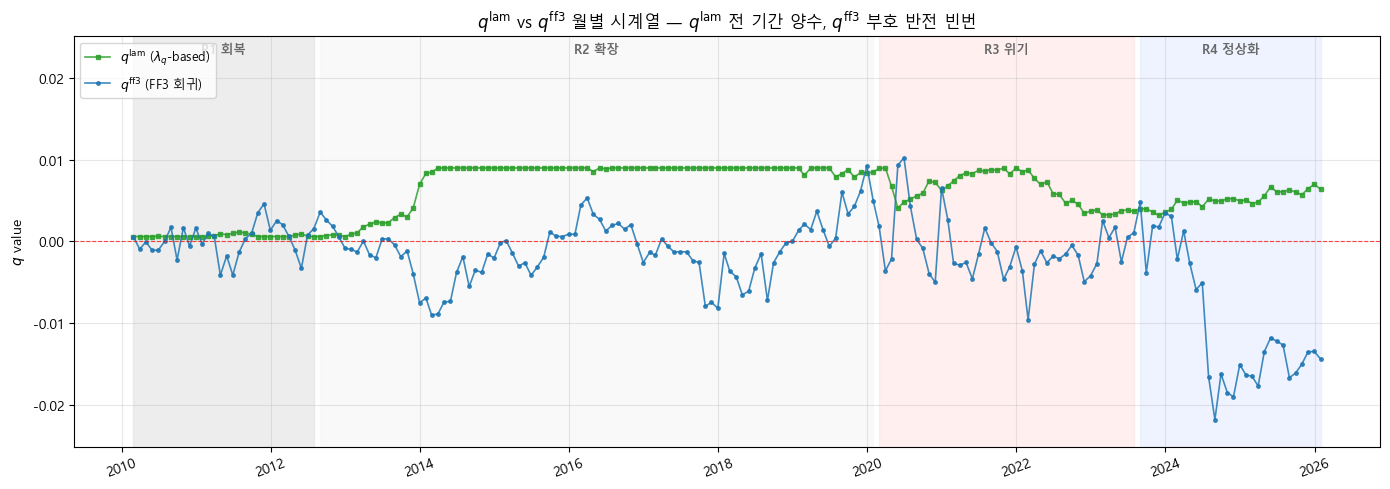
\includegraphics[width=0.95\textwidth]{Figure/r4_ff3_lam.png}
\caption{$q^{\mathrm{ff3}}$(파란 원, FF3 회귀 기반)과 $q^{\mathrm{lam}}$(초록 사각, $\lambda_q$ 기반)의 월별 시계열 — 앵커 슬롯 \texttt{mcap\_mcap\_ff3\_err} 기준. 빨간 점선은 부호 반전 임계선(0), 음영은 4개 국면. $q^{\mathrm{lam}}$은 전 기간 양수를 유지하나, $q^{\mathrm{ff3}}$은 빈번한 부호 반전 후 R4 국면에서 강한 음수로 수렴한다.}
\label{fig:q_timeline}
\end{figure}

그림~\ref{fig:q_timeline} 은 \citet{pyo2018} 가 제안한 앵커 슬롯의 $q^{\mathrm{ff3}}$ 과 동일 앵커에서 $q$ 만 $q^{\mathrm{lam}}$ 으로 교체한 경우의 값을 시각화한 것이다. FF3 기반의 $q^{\mathrm{ff3}}$ 은 R1\textendash R3 구간에서도 부호 반전을 자주 보이며 R4 에 들어서면 0 아래에 머물러 뷰 방향이 반전된 상태가 유지되는 반면,
양수 clip 범위를 갖는 $\lambda_q$ 기반의 $q^{\mathrm{lam}}$ (\ref{subsubsec:bl_proposed_slot}절 정의) 은 전 기간 양수를 유지하여 저변동 뷰의 일관성을 보존한다.

\subsection{$\mathbf{p}$ 벡터 변경의 완화 효과}

R4 정상화 국면에서 $\mathbf{w}_{mkt} = \mathbf{w}^{\mathrm{mcap}}, \omega = \omega^{\mathrm{err}}$을 고정한 채 $\mathbf{p}$ 와 $q$를 변경한 모든 조합의 스프레드는 다음과 같다(앙상블 기준).

\begin{table}[t]
\centering
\caption{R4 정상화 구간에서 $\mathbf{w}_{mkt} = \mathbf{w}^{\mathrm{mcap}}, \omega = \omega^{\mathrm{err}}$ 고정 후 $\mathbf{p}$ 와 $q$를 변경한 모든 조합의 스프레드(저변동 $-$ 고변동, 앙상블 기준).
$(\mathbf{p}^{\mathrm{mcap}}, q^{\mathrm{ff3}})$ 한 조합에서만 음수로 반전된다.}
\label{tab:r4_pq_spread}
\setlength{\tabcolsep}{10pt}
\renewcommand{\arraystretch}{1.2}
\small
\begin{tabular}{lccccc}
\toprule
스프레드 (저$-$고) & $q^{\mathrm{lam}}$ & $q^{\mathrm{raw}}$ & $q^{\mathrm{inv}}$ & $q^{\mathrm{vsp}}$ & $q^{\mathrm{ff3}}$ \\
\midrule
$\mathbf{p}^{\mathrm{mcap}}$ & $+0.290$ & $+0.290$ & $+0.229$ & $+0.236$ & $\mathbf{-0.145}$ \\
$\mathbf{p}^{\mathrm{eq}}$   & $+0.335$ & $+0.335$ & $+0.267$ & $+0.278$ & $+0.146$ \\
$\mathbf{p}^{\mathrm{rp}}$   & $+0.332$ & $+0.332$ & $+0.265$ & $+0.277$ & $+0.153$ \\
\bottomrule 
\end{tabular}
\end{table}

R4 국면에서 스프레드가 음수로 전환되는 조합은 $(\mathbf{p}^{\mathrm{mcap}}, q^{\mathrm{ff3}})$ 단 1개에 불과하며, 동일한 $q^{\mathrm{ff3}}$을 사용하더라도 $\mathbf{p}$를 $\mathbf{p}^{\mathrm{eq}}$ 또는 $\mathbf{p}^{\mathrm{rp}}$로 변경하면 스프레드가 양수($+0.146, +0.153$)로 회복된다. ANN 기준에서도 같은 패턴이 관찰되며($\mathbf{p}^{\mathrm{mcap}} \cdot q^{\mathrm{ff3}}$: $-0.103$, $\mathbf{p}^{\mathrm{eq}} \cdot q^{\mathrm{ff3}}$: $+0.165$, $\mathbf{p}^{\mathrm{rp}} \cdot q^{\mathrm{ff3}}$: $+0.179$), 양수 제약이 있는 $q$와 결합된 $\mathbf{p}$는 모든 조합에서 스프레드 $0.20$\textendash $0.34$ 수준의 저변동 우위 뷰를 유지한다.

즉, R4 국면에서 저변동 전략 본질의 반전은 $\mathbf{p}^{\mathrm{mcap}}$ 가중과 $q^{\mathrm{ff3}}$의 결합 조건에서만 관찰되며, 두 요소 중 어느 한쪽이라도 변경되면 저변동 본질이 부분적 또는 완전 회복된다.

\section{벤치마크 대비 보조 지표}\label{app:benchmark}

\ref{subsec:benchmark}절(벤치마크 성능 비교)에서 보고한 샤프 비율 결과(표~\ref{tab:benchmark_sharpe})에 대응하여, 동일한 슬롯과 5개 기간(All, R1 회복, R2 확장, R3 위기, R4 정상화)에 대한 보조 지표 3종을 첨부한다.  표~\ref{tab:benchmark_sortino}는 Sortino 비율, 표~\ref{tab:benchmark_mdd} 는 최대낙폭 (MDD), 표~\ref{tab:benchmark_annret}은 연환산 수익률을 보고하며, 각 표에서 4개 앙상블 슬롯 중 컬럼별 최우수 값을 굵게 표시한다. Sortino 비율과 연환산 수익률은 클수록, MDD는 0에 가까울수록 우위이다.

% ── Sortino 비율 ───────────────────────────────────────────
\begin{table}[t]
\centering
\caption{벤치마크 성능 비교 — Sortino 비율 $\times$ 5기간. 4개 앙상블 슬롯 중 컬럼별 최대값 굵게 표시.}
\label{tab:benchmark_sortino}
\setlength{\tabcolsep}{6pt}
\renewcommand{\arraystretch}{1.15}
\small
\begin{tabular}{lccccc}
\toprule
Strategy & All & R1 & R2 & R3 & R4 \\
\midrule
SPY (market)                       & 1.38 & 1.41 & 1.66 & 1.06 & 2.36 \\
$1/N$ (equal-weight)               & 1.21 & 1.32 & 1.47 & 1.08 & 0.88 \\
Risk Parity ($1/\sigma$)           & 1.25 & 1.72 & 1.50 & 1.05 & 0.81 \\
ANN-anchor \citep{pyo2018}         & 1.34 & 1.56 & 1.36 & 1.60 & 0.88 \\
Ensemble-anchor ($\sigma$ 모형 교체) & 1.32 & 1.19 & 1.48 & 1.17 & 1.51 \\
\midrule
\textbf{Ensemble-defensive} ($\mathbf{p}^{\mathrm{eq}}, q^{\mathrm{lam}}$) & \textbf{1.66} & \textbf{1.78} & \textbf{1.82} & \textbf{1.80} & 0.98 \\
\textbf{Ensemble-defensive} ($\mathbf{p}^{\mathrm{rp}}, q^{\mathrm{lam}}$) & 1.64          & 1.67          & 1.75          & 1.79          & 1.10 \\
\textbf{Ensemble-adaptive}  ($\mathbf{p}^{\mathrm{eq}}, q^{\mathrm{ff3}}$) & 1.62          & 1.47          & 1.70          & 1.77          & 1.72 \\
\textbf{Ensemble-adaptive}  ($\mathbf{p}^{\mathrm{rp}}, q^{\mathrm{ff3}}$) & 1.59          & 1.44          & 1.64          & 1.75          & \textbf{1.78} \\
\bottomrule
\end{tabular}
\end{table}

% ── 최대낙폭 (MDD) ─────────────────────────────────────────
\begin{table}[t]
\centering
\caption{벤치마크 성능 비교 — 최대낙폭 (MDD) $\times$ 5 기간 (0에 가까울수록 우위).
4개 앙상블 슬롯 중 컬럼별 최우수(절대값 최소) 굵게 표시.}
\label{tab:benchmark_mdd}
\setlength{\tabcolsep}{6pt}
\renewcommand{\arraystretch}{1.15}
\small
\begin{tabular}{lccccc}
\toprule
Strategy & All & R1 & R2 & R3 & R4 \\
\midrule
SPY (market)                       & $-23.9\%$ & $-16.2\%$ & $-13.5\%$ & $-23.9\%$ & $-7.6\%$  \\
$1/N$ (equal-weight)               & $-24.3\%$ & $-21.4\%$ & $-17.3\%$ & $-16.8\%$ & $-12.0\%$ \\
Risk Parity ($1/\sigma$)           & $-22.0\%$ & $-18.2\%$ & $-15.8\%$ & $-16.1\%$ & $-10.4\%$ \\
ANN-anchor \citep{pyo2018}         & $-18.4\%$ & $-12.5\%$ & $-16.1\%$ & $-16.1\%$ & $-18.4\%$ \\
Ensemble-anchor ($\sigma$ 모형 교체) & $-20.5\%$ & $-17.1\%$ & $-17.6\%$ & $-16.5\%$ & $-14.0\%$ \\
\midrule
\textbf{Ensemble-defensive} ($\mathbf{p}^{\mathrm{eq}}, q^{\mathrm{lam}}$) & $-14.7\%$          & $\mathbf{-12.8\%}$ & $\mathbf{-8.2\%}$ & $-14.7\%$          & $-8.9\%$ \\
\textbf{Ensemble-defensive} ($\mathbf{p}^{\mathrm{rp}}, q^{\mathrm{lam}}$) & $\mathbf{-14.0\%}$ & $-14.0\%$          & $-8.5\%$          & $\mathbf{-13.4\%}$ & $-8.7\%$ \\
\textbf{Ensemble-adaptive}  ($\mathbf{p}^{\mathrm{eq}}, q^{\mathrm{ff3}}$) & $-15.7\%$          & $-15.7\%$          & $-11.4\%$         & $-15.1\%$          & $-7.9\%$ \\
\textbf{Ensemble-adaptive}  ($\mathbf{p}^{\mathrm{rp}}, q^{\mathrm{ff3}}$) & $-19.2\%$          & $-19.2\%$          & $-12.6\%$         & $-15.0\%$          & $\mathbf{-7.5\%}$ \\
\bottomrule
\end{tabular}
\end{table}

% ── 연환산 수익률 ──────────────────────────────────────────
\begin{table}[t]
\centering
\caption{벤치마크 성능 비교 — 연환산 수익률 $\times$ 5 기간. 4개 앙상블 슬롯 중 컬럼별 최대값 굵게 표시.}
\label{tab:benchmark_annret}
\setlength{\tabcolsep}{6pt}
\renewcommand{\arraystretch}{1.15}
\small
\begin{tabular}{lccccc}
\toprule
Strategy & All & R1 & R2 & R3 & R4 \\
\midrule
SPY (market)                       & $+14.4\%$ & $+12.7\%$ & $+14.2\%$ & $+12.4\%$ & $+19.7\%$ \\
$1/N$ (equal-weight)               & $+14.8\%$ & $+14.3\%$ & $+16.1\%$ & $+15.5\%$ & $+10.5\%$ \\
Risk Parity ($1/\sigma$)           & $+14.2\%$ & $+14.9\%$ & $+15.6\%$ & $+13.9\%$ & $+9.8\%$  \\
ANN-anchor \citep{pyo2018}         & $+14.3\%$ & $+16.6\%$ & $+12.9\%$ & $+15.0\%$ & $+15.2\%$ \\
Ensemble-anchor ($\sigma$ 모형 교체) & $+15.1\%$ & $+11.4\%$ & $+15.9\%$ & $+14.2\%$ & $+17.9\%$ \\
\midrule
\textbf{Ensemble-defensive} ($\mathbf{p}^{\mathrm{eq}}, q^{\mathrm{lam}}$) & $+15.1\%$          & $\mathbf{+17.2\%}$ & $+15.1\%$          & $\mathbf{+16.7\%}$ & $+11.1\%$ \\
\textbf{Ensemble-defensive} ($\mathbf{p}^{\mathrm{rp}}, q^{\mathrm{lam}}$) & $+14.7\%$          & $+15.2\%$          & $+14.7\%$          & $+16.5\%$          & $+11.9\%$ \\
\textbf{Ensemble-adaptive}  ($\mathbf{p}^{\mathrm{eq}}, q^{\mathrm{ff3}}$) & $\mathbf{+15.9\%}$ & $+14.0\%$          & $\mathbf{+16.4\%}$ & $+15.7\%$          & $+16.4\%$ \\
\textbf{Ensemble-adaptive}  ($\mathbf{p}^{\mathrm{rp}}, q^{\mathrm{ff3}}$) & $+15.3\%$          & $+13.1\%$          & $+15.6\%$          & $+15.3\%$          & $\mathbf{+16.8\%}$ \\
\bottomrule
\end{tabular}
\end{table}

%%%%%%%%%%%%%%%%%%%%%%%%%%%%%%%%%%%%%%%%%%%%%%%%%%%%%%%%%%%%%%%%%%%%%
%%  국문 요약 (마지막 페이지에 자동 배치됨)
%%%%%%%%%%%%%%%%%%%%%%%%%%%%%%%%%%%%%%%%%%%%%%%%%%%%%%%%%%%%%%%%%%%%%
\newpage

\begin{reference}
%
% Journal articles
%
\bibitem[Andersen et al.(2003)]{andersen2003modeling}Andersen TG, Bollerslev T, Diebold FX, and Labys P (2003).
Modeling and forecasting realized volatility,
\textit{Econometrica}, \textbf{71}, 579--625.

\bibitem[Baker et al.(2011)]{baker2011}Baker M, Bradley B, and Wurgler J (2011).
Benchmarks as limits to arbitrage: Understanding the low-volatility anomaly,
\textit{Financial Analysts Journal}, \textbf{67}, 40--54.

\bibitem[Barua and Sharma(2023)]{barua2023using}Barua R and Sharma AK (2023).
Using fear, greed and machine learning for optimizing global portfolios: A Black-Litterman approach,
\textit{Finance Research Letters}, \textbf{58}, 104515.

\bibitem[Bates and Granger(1969)]{bates1969combination}Bates JM and Granger CWJ (1969).
The combination of forecasts,
\textit{Journal of the Operational Research Society}, \textbf{20}, 451--468.

\bibitem[Black and Litterman(1992)]{black1992}Black F and Litterman R (1992).
Global portfolio optimization,
\textit{Financial Analysts Journal}, \textbf{48}, 28--43.

\bibitem[Blitz and van Vliet(2007)]{blitz2007}Blitz DC and van Vliet P (2007).
The volatility effect: Lower risk without lower return,
\textit{The Journal of Portfolio Management}, \textbf{34}, 102--113.

\bibitem[Bucci(2020)]{bucci2020realized}Bucci A (2020).
Realized volatility forecasting with neural networks,
\textit{Journal of Financial Econometrics}, \textbf{18}, 502--531.

\bibitem[Cont(2001)]{cont2001}Cont R (2001).
Empirical properties of asset returns: stylized facts and statistical issues,
\textit{Quantitative Finance}, \textbf{1}, 223--236.

\bibitem[Corsi(2009)]{corsi2009}Corsi F (2009).
A simple approximate long-memory model of realized volatility,
\textit{Journal of Financial Econometrics}, \textbf{7}, 174--196.

\bibitem[DeMiguel et al.(2009)]{demiguel2009optimal}DeMiguel V, Garlappi L, and Uppal R (2009).
Optimal versus naive diversification: How inefficient is the 1/N portfolio strategy?,
\textit{The Review of Financial Studies}, \textbf{22}, 1915--1953.

\bibitem[Fama and French(1993)]{fama1993common}Fama EF and French KR (1993).
Common risk factors in the returns on stocks and bonds,
\textit{Journal of Financial Economics}, \textbf{33}, 3--56.

\bibitem[Fama and MacBeth(1973)]{fama1973risk}Fama EF and MacBeth JD (1973).
Risk, return, and equilibrium: Empirical tests,
\textit{Journal of Political Economy}, \textbf{81}, 607--636.

\bibitem[Frazzini and Pedersen(2014)]{frazzini2014}Frazzini A and Pedersen LH (2014).
Betting against beta,
\textit{Journal of Financial Economics}, \textbf{111}, 1--25.

\bibitem[Gers et al.(2000)]{gers2000}Gers FA, Schmidhuber J, and Cummins F (2000).
Learning to forget: Continual prediction with LSTM,
\textit{Neural Computation}, \textbf{12}, 2451--2471.

\bibitem[Hamilton(1989)]{hamilton1989new}Hamilton JD (1989).
A new approach to the economic analysis of nonstationary time series and the business cycle,
\textit{Econometrica}, \textbf{57}, 357--384.

\bibitem[Hochreiter and Schmidhuber(1997)]{hochreiter1997}Hochreiter S and Schmidhuber J (1997).
Long short-term memory,
\textit{Neural Computation}, \textbf{9}, 1735--1780.

\bibitem[Kim and Won(2018)]{kim2018forecasting}Kim HY and Won CH (2018).
Forecasting the volatility of stock price index: A hybrid model integrating LSTM with multiple GARCH-type models,
\textit{Expert Systems with Applications}, \textbf{103}, 25--37.

\bibitem[Ledoit and Wolf(2004)]{ledoitwolf2004}Ledoit O and Wolf M (2004).
A well-conditioned estimator for large-dimensional covariance matrices,
\textit{Journal of Multivariate Analysis}, \textbf{88}, 365--411.

\bibitem[Lee et al.(2025)]{lee2025llm}Lee Y, Kim Y, Kim J, Kim S, and Lee Y (2025).
LLM-Enhanced Black-Litterman Portfolio Optimization,
\textit{arXiv preprint arXiv:2504.14345}.

\bibitem[Maillard et al.(2010)]{maillard2010}Maillard S, Roncalli T, and Te\"iletche J (2010).
The properties of equally weighted risk contribution portfolios,
\textit{The Journal of Portfolio Management}, \textbf{36}, 60--70.

\bibitem[Markowitz(1952)]{markowitz1952}Markowitz H (1952).
Portfolio selection,
\textit{The Journal of Finance}, \textbf{7}, 77--91.

\bibitem[M\"uller et al.(1997)]{muller1997}M\"uller UA, Dacorogna MM, Dav\'e RD, Olsen RB, Pictet OV, and von Weizs\"acker JE (1997).
Volatilities of different time resolutions---Analyzing the dynamics of market components,
\textit{Journal of Empirical Finance}, \textbf{4}, 213--239.

\bibitem[Pyo and Lee(2018)]{pyo2018}Pyo S and Lee J (2018).
Exploiting the low-risk anomaly using machine learning to enhance the Black-Litterman framework,
\textit{Pacific-Basin Finance Journal}, \textbf{51}, 1--12.

\bibitem[Rumelhart et al.(1986)]{rumelhart1986learning}Rumelhart DE, Hinton GE, and Williams RJ (1986).
Learning representations by back-propagating errors,
\textit{Nature}, \textbf{323}, 533--536.

\bibitem[Sortino and Price(1994)]{sortino1994}Sortino FA and Price LN (1994).
Performance measurement in a downside risk framework,
\textit{The Journal of Investing}, \textbf{3}, 59--64.

\bibitem[Su et al.(2026)]{su2026objective}Su X, Lu K, and Yen J (2026).
Objective Black-Litterman views through deep learning: A novel hybrid model for enhanced portfolio returns,
\textit{Expert Systems with Applications}, \textbf{295}, 128868.

\bibitem[Whaley(2009)]{whaley2009understanding}Whaley RE (2009).
Understanding the VIX,
\textit{Journal of Portfolio Management}, \textbf{35}, 98--105.

\bibitem[Yu et al.(2019)]{yu2019review}Yu Y, Si X, Hu C, and Zhang J (2019).
A review of recurrent neural networks: LSTM cells and network architectures,
\textit{Neural Computation}, \textbf{31}, 1235--1270.

%
% Books
%
\bibitem[Cochrane(2005)]{cochrane2005}Cochrane JH (2005).
\textit{Asset Pricing} (Revised ed.), Princeton University Press, Princeton.

\bibitem[L\'opez de Prado(2018)]{lopezdeprado2018}L\'opez de Prado M (2018).
\textit{Advances in Financial Machine Learning}, John Wiley \& Sons, Hoboken.

%
% Book chapters
%
\bibitem[Timmermann(2006)]{timmermann2006forecast}Timmermann A (2006).
Forecast combinations. In Elliott G, Granger CWJ, and Timmermann A (Eds),
\textit{Handbook of Economic Forecasting} (Vol. 1, pp. 135--196), Elsevier, Amsterdam.

%
% Technical reports
%
\bibitem[He and Litterman(1999)]{helitterman1999}He G and Litterman R (1999).
The intuition behind Black-Litterman model portfolios,
Goldman Sachs Investment Management Research.

\end{reference}


\htitle{변동성 예측을 결합한 블랙-리터만 저변동성 포트폴리오 전략}

\hauthor{
서윤범\address[a]{팀스파르타;},
김하연\same[a],
김재천\same[a],
김윤서\same[a],
서정욱\footnote{교신저자: (15588) 경기도 안산시 한양대학로 55, 한양대학교 응용인공지능학과. E-mail: sju02051@hanyang.ac.kr}\address[b]{한양대학교 응용인공지능학과}
}

\begin{habstract}
블랙-리터만(Black-Litterman, BL) 모형은 시장 균형에 투자자 뷰를 결합하여 평균-분산 최적화의 추정 오차 민감성을 완화하지만, 뷰가 전문가의 주관에 의존한다는 한계를 갖는다. 이를 보완하기 위한 머신러닝 기반 BL 응용 연구가 활발하나 대부분 수익률 예측에 집중되어 있고, 변동성 예측을 직접 뷰로 활용하는 연구는 제한적이다. 본 연구는 인공신경망(ANN) 기반 변동성 예측을 BL 뷰로 결합한 Pyo와 Lee (2018)의 프레임워크를 출발점으로, 두 축으로 확장한다: (1) 단순 ANN을 LSTM과 HAR의 앙상블로 대체하여 시계열 의존 구조를 반영하고, (2) BL의 네 입력 슬롯 ($\mathbf{p}, q, \omega, \mathbf{w}_{mkt}$) 을 각각 복수의 후보로 정의해 곱집합으로 결합한 90개 슬롯 조합을 체계적으로 탐색한다. 2010--2025년 S\&P 500 617 종목, 192개월 실증 분석에서 LSTM-HAR 앙상블은 ANN 대비 변동성 예측 정확도에서 일관된 우위를 보였으며 특히 COVID-19가 포함된 위기 구간(R3)에서 격차가 가장 크게 확대되었다. 이 예측 우위가 포트폴리오 성과로 전이되기 위해서는 뷰 포트폴리오의 대형주 비중 집중 완화($\mathbf{p}^{\mathrm{eq}}, \mathbf{p}^{\mathrm{rp}}$) 가 결정적임을 확인하였다. 본 연구가 제안하는 두 슬롯 옵션 --- 모든 시장 국면에서 저변동 뷰를 일관되게 유지하는 Ensemble-defensive (샤프 비율 1.04--1.07) 와 강세장 적응을 허용하는 Ensemble-adaptive (샤프 비율 1.05--1.10) --- 는 편측 20bp 거래비용 차감 후에도 SPY (0.93), $1/N$ (0.86), Risk Parity (0.89), ANN-anchor (0.95) 를 모두 상회한다. 본 연구는 90 슬롯의 차원별 주변 분포와 국면별 결과 분석을 통해 변동성 기반 BL 저변동 전략의 운용 목표별 슬롯 선택 근거를 제시한다.
\end{habstract}

\hkeywords{블랙-리터만, 변동성 예측, LSTM, HAR, 저변동 포트폴리오}

\end{document}
